\documentclass[a4paper,12pt]{report}

\usepackage{graphicx}
\usepackage[utf8]{inputenc}
\usepackage[italian]{babel}
\usepackage{geometry}
\usepackage{setspace}
\usepackage{titlesec}
\usepackage{fontspec}
\usepackage{subfig}
\usepackage{tikz}
\usepackage{caption}
\usepackage{listings}
\usepackage{enumitem}
\usepackage{float}
\usepackage{natbib}
\usepackage{quotchap}



\captionsetup{
  font=small, % Imposta il font delle didascalie come "small" (piccolo)
  justification=centering, % Allinea le didascalie al centro
  singlelinecheck=false, % Permette alle didascalie di occupare più righe se necessario
  skip=5pt % Aggiunge uno spazio verticale di 5pt tra la figura e la didascalia
}

\setmainfont{Calibri}

\geometry{
  a4paper,
  left=4.5cm,
  right=3cm,
  top=4cm,
  bottom=4cm,
}

\lstset{
    language=Python,
    basicstyle=\ttfamily\small,
    keywordstyle=\color{blue},
    commentstyle=\color{green!40!black},
    stringstyle=\color{orange},
    showstringspaces=false,
    breaklines=true,
    frame=single,
    numbers=left,
    numberstyle=\tiny,
    captionpos=b,
    lineskip=1pt
}

\titleformat{\section}
  {\fontsize{14}{16}\bfseries}
  {\thesection}
  {1em}
  {}

\titleformat{\subsection}
  {\fontsize{12}{14}\bfseries}
  {\thesubsection}
  {1em}
  {}

\linespread{1.5}
\setlength{\parindent}{0pt}

\begin{document}
\selectlanguage{italian}

\begin{titlepage}
\centering

\textbf{\large Università degli Studi di Bari} \\
\vspace{0.3cm}
\textbf{\large Dipartimento di Informatica} \\
\vspace{1cm}

\includegraphics[width=40mm,scale=0.5]{assets/images/logo.png} \\
\vspace{1cm}
\textbf{\large Tesi di Laurea Triennale in Informatica e Tecnologie per la Produzione del Software} \\
\vspace{1cm}
\textbf{\LARGE Upgrade del Sistema di Foto Identificazione Automatica SPIR: Porting, Intelligenza Artificiale e Ottimizzazione dell'Interfaccia Utente} \\
\vspace{0.7cm}
\textbf{\large Autore:} \\
\textbf{Antonio Ricciardi} \\
\vspace{0.3cm}
\textbf{\large Relatore:} \\
Prof. \textbf{Giovanni Dimauro} \\
\vspace{0.3cm}
\textbf{\large Correlatori:} \\
Dott.ssa \textbf{Rosalia Maglietta} \\
Dott.ssa \textbf{Carla Cherubini} \\
\vfill
\vspace{0.3cm}
\textbf{Anno Accademico 2022/2023} % Inserisci l'anno accademico corretto
    
\end{titlepage}
\clearpage
\thispagestyle{empty}

\vspace*{\fill}
\begin{center}
\textit{“Make everything as simple as possible, but not simpler.”\\
- ALBERT EINSTEIN}
\end{center}
\vfill
\clearpage
\tableofcontents

\chapter{Introduzione}


  Il presente lavoro di tesi può essere contestualizzato nell’ambito di una disciplina emergente che coniuga l'informatica con
  l'ecologia, nota come "ecoinformatica". Questo nuovo campo scientifico unisce la crescente capacità delle tecnologie 
  dell’informazione di sfruttare dati complessi allo studio di processi ecologici ed ambientali. Essa risponde all'imperativo di accelerare
  l’avvento di processi sostenibili in vista dei cambiamenti climatici e ambientali
  globali.
  Ad oggi, gli ecosistemi del globo stanno sperimentando dei cambiamenti senza precedenti che minacciano la biodiversità del pianeta
  ed i servizi ecosistemici ed economici che fornisce alla popolazione umana. 
  \newpage
  \begin{figure}[H]
    \centering
    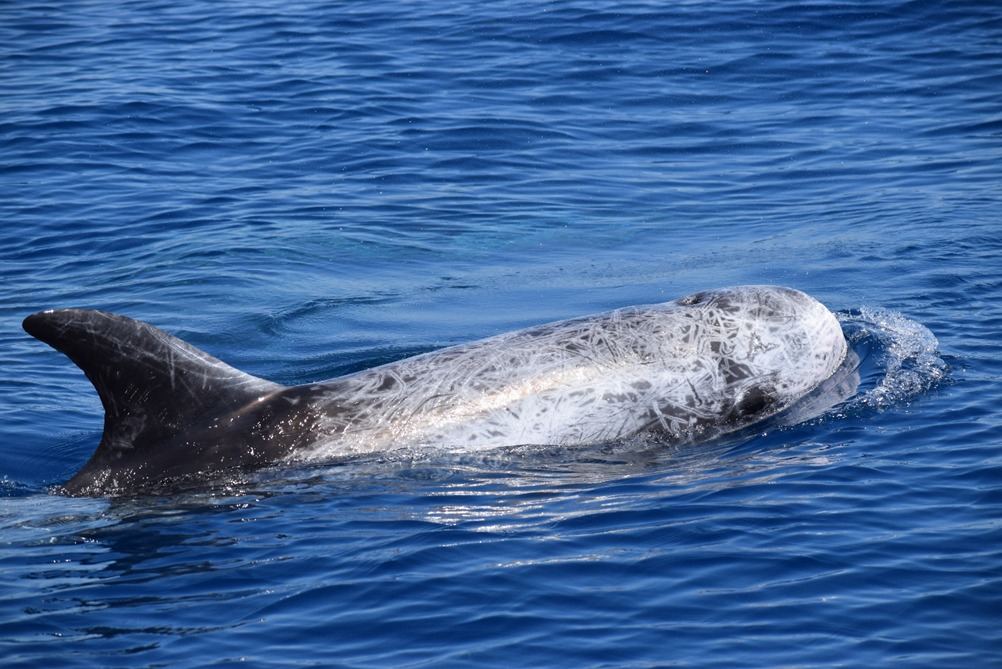
\includegraphics[width=\textwidth]{assets/images/intro/intro.jpeg}   
    \caption{Esemplare di delfino Risso}
  \end{figure}

  Tra gli innumerevoli fattori responsabili di tali cambiamenti sono annoverati
  il cambiamento climatico, la degradazione degli habitat ad opera dell'uomo, le varie forme di inquinamento (chimico, fisico, biologico), 
  l'estinzione di specie. Tutte queste minacce contribuiscono ad alimentare un circuito a feedback positivo, 
  che pone in serio pericolo il benessere e la sopravvivenza stessa dell'essere umano, la cui economia è strettamente
  legata allo sfruttamento di risorse naturali che si stanno via via impoverendo (sia qualitativamente che quantitativamente). Inoltre, 
  in uno scenario di cambiamento climatico sempre più allarmante, risulta ormai essenziale lo sviluppo di soluzioni basate sulla
  natura per contrastare sia riscaldamento globale che il trend di declino degli ecosistemi. Poichè è ampiamente dimostrato che la salute dell'essere umano è strettamente
  connessa a quella dell'ambiente e delle specie che lo popolano, risulta urgente e di fondamentale importanza accellerare e implementare i processi di
  monitoraggio degli ecosistemi grazie all'utilizzo di tecnologie innovative e all'avanguardia.
  
  L'ambiente marino è uno degli habitat più minacciati del pianeta.
  \newpage
  Appare quindi necessario 
  studiare con particolare attenzione le specie marine
  vulnerabili che utilizzano tale ambiente al fine di comprendere come esse possono reagire ai rapidi cambiamenti in atto. 
  A tal proposito, la tecnica di foto identificazione rientra tra le metodologie maggiormente
  utilizzate e più efficaci per monitorare nel tempo specie d'interesse conservazionistico e elusive, 
  come i cetacei. Questi animali svolgono un ruolo fondamentale nella conservazione della biodiversità marina, mantenendo la stabilità 
  degli ecosistemi marini grazie al loro ruolo di predatori di vertice nelle reti alimentari.
  La foto identificazione (photo ID) è una tecnica non invasiva dedicata all'identificazione 
  di singoli esemplari tramite foto. Si basa sull'ipotesi che ogni esemplare abbia caratteristiche uniche che consentano il suo riconoscimento.
  Le informazioni ottenute con gli studi di photo ID sono utili per effettuare una stima della abbondanza delle popolazioni di specie studiate,
  sulle loro dinamiche sociali e movimenti migratori, così da contribuire in modo efficace alle misure di gestione e conservazione delle suddette specie.
  \\
  Un limite che ostacola l'utilizzo e l'applicazione della tecnica della foto identificazione manuale è che essa
  richiede molto tempo ed è poco pratica nel caso di grandi insiemi di dati. Per ridurre il tempo e lo sforzo dell'utente necessario a
  identificare e riconoscere gli individui incontrati, sono stati pertanto sviluppati dei sistemi tecnologici automatizzati e intelligenti
  finalizzati a supportare i ricercatori nella foto identificazione. Nel caso specifico della foto identificazione dei cetacei che si basa sull'utilizzo
  delle pinne dorsali degli individui fotografati, l'elaborazione automatica di queste immagini prevede diverse fasi: una fase di rilevamento dell'oggetto, un ritaglio della pinna, la segmentazione e l'estrazione della maschera. Successivamente, 
  se richiesto, può essere eseguita l'estrazione delle caratteristiche, seguita dal riconoscimento individuale. I sistemi semi-automatici ed automatici di foto identificazione
  per i cetacei sono stati esaustivamente elencati nella review della letteratura condotta da \cite{maglietta2022machine}. 
  Il presente lavoro di tesi ha voluto sviluppare un'implementazione del sistema SPIR (Smart Photo Identification of the Risso’s dolphin) \cite{maglietta2018dolfin}, 
  che rappresenta un sistema completamente automatizzato inizialmente sviluppato
  per studiare la presenza del delfino di Risso (\textit{Grampus griseus}) nel Golfo di Taranto, specie classificata come 'Minacciata' dalla Red List della IUCN \cite{lanfredi2021grampus}. 
  I delfini di Risso infatti sono distribuiti dai 
  tropici fino alle regioni temperate in entrambi gli emisferi terrestri. Un individuo in 
  età adulta può avere una lunghezza compresa tra 2,5 e 4 metri ed un peso di 500-
  600 kg. A differenza di altri odontoceti, come i tursiopi, il capo si presenta sprovvisto di rostro 
  e con un largo sfiatatoio nella parte superiore. L’intero corpo di questi delfini, pinna dorsale 
  inclusa, è generalmente ricoperto da una quantità notevole di graffi di tonalità 
  molto chiara. La comparsa di questi segni avviene in modo graduale nel corso della 
  vita dell’animale (alla nascita, infatti, il colore del corpo è grigio scuro e uniforme) ed è molto probabilmente 
  collegata ad interazioni sia di carattere sociale che alimentare. La presenza di graffi sulla superficie della pinna dorsale degli individui è proprio 
  il tratto fisico distintivo che consente di 
  applicare la tecnica di foto-identificazione agli esemplari di grampo. Ogni animale presenta un pattern di segni unico che lo 
  contraddistingue individualmente all'interno della popolazione.

  L'originale versione del sistema SPIR (MATLAB) consente di effettuare l’identificazione degli esemplari di 
  grampo non noti basandosi su un dataset di esemplari precedentemente identificati senza alcun intervento da parte dell’utente. SPIR opera secondo i seguenti 
  step principali:
  \begin{itemize}
    \item Utilizza in input immagini contenenti una pinna dorsale, ritagliate ad hoc a 
    partire dagli scatti collezionati durante le campagne di raccolta dati
    in mare;      
    \item Applica algoritmi di feature extraction in grado di ottenere una 
    rappresentazione dell’identità dell’individuo in termini di "descrittori" calcolati 
    a partire dai graffi presenti sulla pinna (Scale
    Invariant Feature Transform (SIFT));
    \item Applica algoritmi di feature matching in grado di associare l’identità degli individui presenti 
    nel database di esemplari già identificati a quella degli esemplari da identificare. 
  
  \end{itemize}



  \section{Obiettivi}
  Il presente lavoro ha come obiettivo principale il miglioramento e l'aggiornamento del sistema di foto-identificazione automatica SPIR (Photo Identification and Recognition System). Per raggiungere tale scopo, sono stati definiti tre obiettivi specifici:
  \begin{itemize}
    \item Realizzazione del porting della versione originale del sistema SPIR:
    Il primo obiettivo del lavoro consiste nel portare la versione esistente del sistema SPIR su una piattaforma più recente o su un linguaggio di programmazione diverso. Ciò garantirà una migliore compatibilità, efficienza e scalabilità del sistema.
    \item Sviluppo di una pipeline con intelligenza artificiale per l'estrazione delle maschere:
    Un secondo obiettivo è l'integrazione di un'Intelligenza Artificiale (IA) all'interno del sistema SPIR per la funzione di estrazione delle maschere. L'utilizzo dell'IA consentirà di migliorare l'accuratezza e l'efficienza dell'estrazione delle maschere, consentendo un'identificazione più precisa e automatizzata delle caratteristiche di interesse nelle foto.
    \item Sviluppo di un'interfaccia grafica user-friendly per il sistema SPIR:
    Infine, un terzo obiettivo è lo sviluppo di un'interfaccia grafica intuitiva e user-friendly per il sistema SPIR. Questo consentirà agli utenti di interagire facilmente con il sistema, fornendo un'esperienza più fluida e accessibile durante l'analisi delle foto e la visualizzazione dei risultati.

  \end{itemize}
  Attraverso il raggiungimento di questi obiettivi, ci si aspetta di ottenere un sistema SPIR migliorato e più efficiente, in grado di supportare efficacemente la foto-identificazione automatica degli esemplari di grampo, nonchè di altre specie di cetacei e di semplificare il lavoro degli operatori, molto spesso biologi ed ecologi, coinvolti nell'analisi delle immagini.


\chapter{Metodi}
  \section{Porting del sistema SPIR}
  Da una prima fase di analisi di SPIR (MATLAB) si nota che l'interazione tra utente e codice è confinata
  a linea di comando (CLI), caratteristica limitante della versione originale del software. Pertanto, in ottica di estendere l'utilizzo di SPIR a una più ampia
  fascia di utenza e, al contempo, mantenere la possibilità di usufruire del codice sorgente, si è optato per una implementazione basata su client/server.
  In particolare, il criterio su cui si è basata l'implementazione del software consiste nello slegare le componenti di interazione e logica del sistema, in modo tale da utilizzare tecnologie più appropriate a seconda del contesto, per poi mettere in comunicazione le 
  varie componenti. Nei seguenti paragrafi sono illustrati i metodi con cui si è effettuato il porting del sistema SPIR.
  \begin{figure}[H]
    \centering
      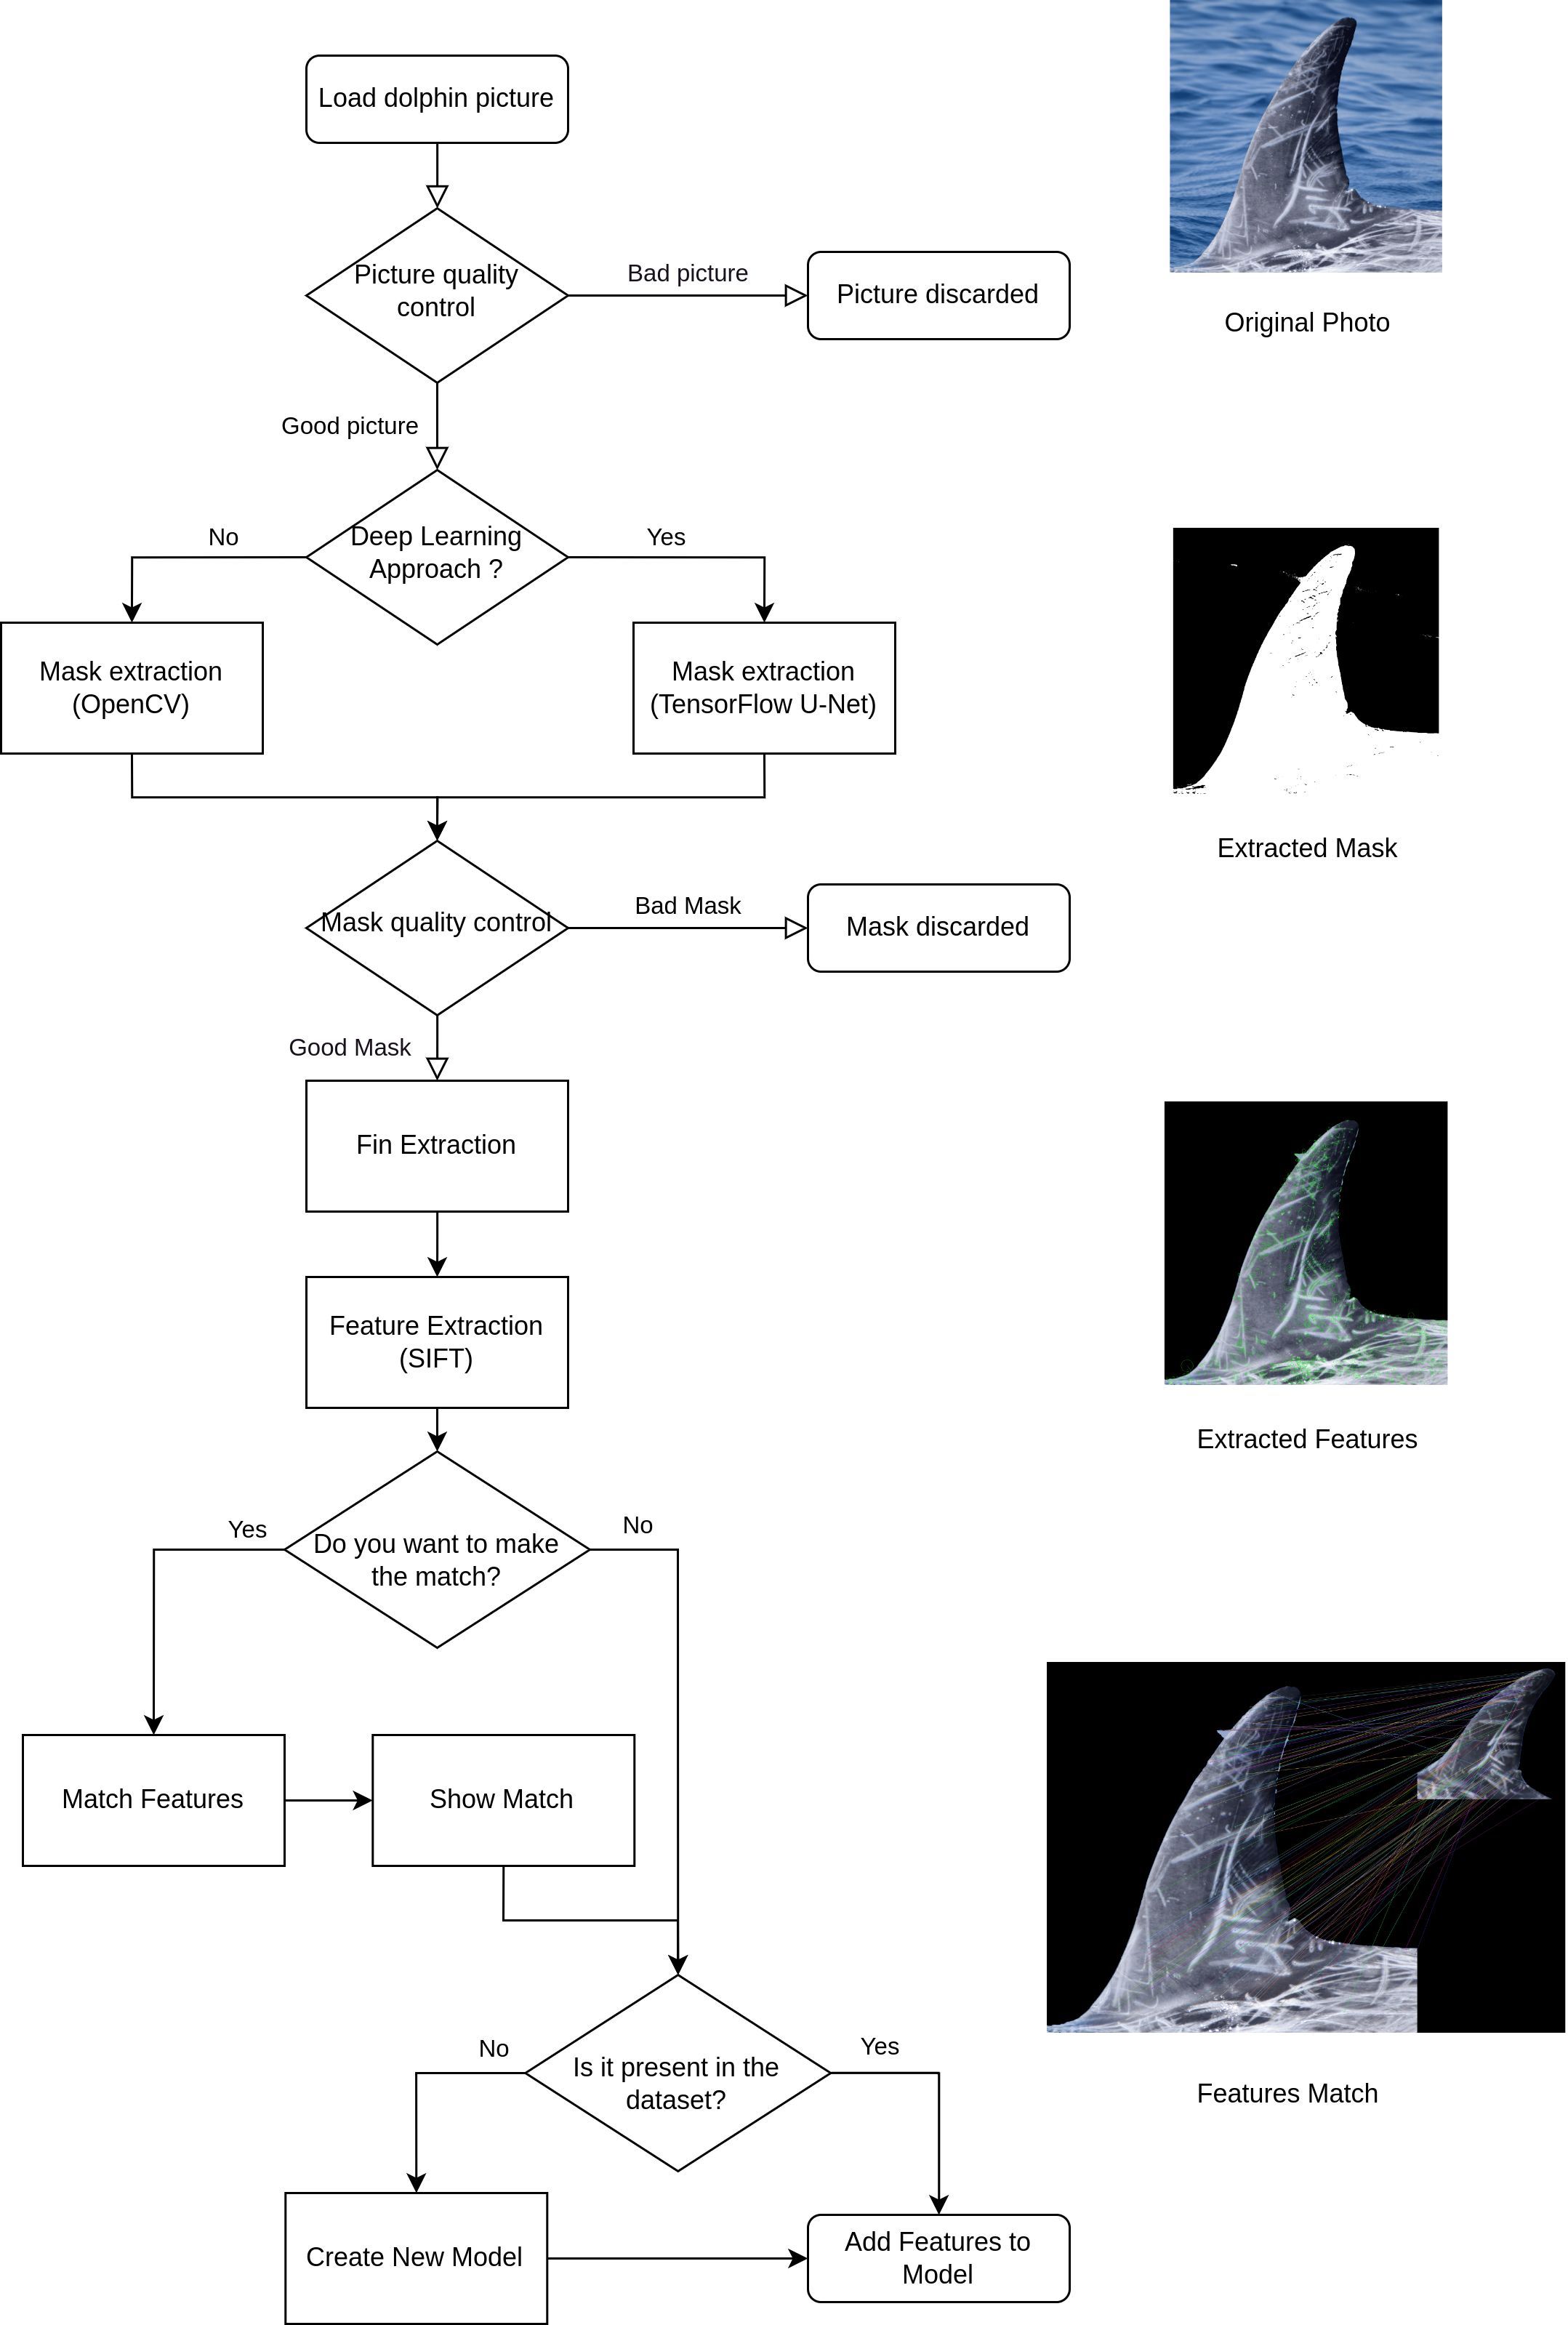
\includegraphics[width=\textwidth]{assets/images/methods/porting/porting_digram.png}  
      \caption{Flowchart SPIR Python}
  \end{figure}

    \subsection{Estrazione della maschera}
      Lo sviluppo di una versione implementata di SPIR si è concentrato inizialmente sulla riscrittura delle sue funzionalità principali.
      Come linguaggio è stato scelto Python per i seguenti motivi:
      \begin{itemize}
        \item Vasta gamma di librerie per la manipolazione di immagini disponibili.
        \item Utilizzo di OpenCV \cite{opencv_library} per l'elaborazione delle immagini.
        \item Buona diffusione in ambito scientifico.
        \item Licenza open source.
        \item Supporto attivo dalla community di sviluppatori.

      \end{itemize}
      
      La prima funzionalità presa in analisi per il porting è stata l'estrazione delle maschere dalle immagini,
      passaggio di fondamentale importanza al fine di ottimizzare l'area di estrazione delle features. L'estrazione delle maschere viene fatta
      nel metodo 
      \begin{verbatim}
prepare_images_vlfeat.m
      \end{verbatim}
      \begin{figure}[H]
        \centering
        
        \begin{minipage}{0.35\textwidth}
          \centering
          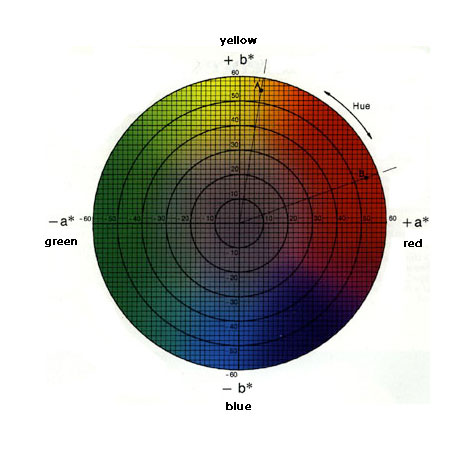
\includegraphics[width=\textwidth]{assets/images/methods/porting/cielab/cielab2.jpg}  
          \caption{Spazio colore CIELAB in 2D}
        \end{minipage}
        \begin{minipage}{0.35\textwidth}
          \centering
          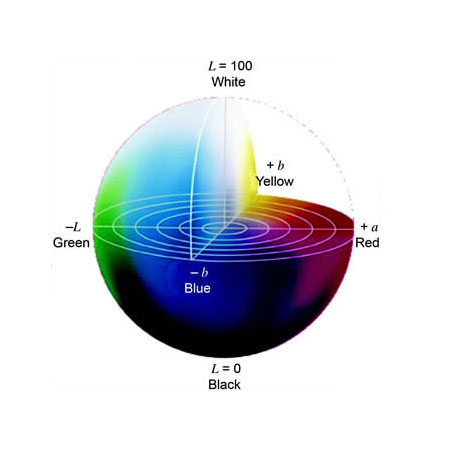
\includegraphics[width=\textwidth]{assets/images/methods/porting/cielab/cielab1.jpg}   
          \caption{Spazio colore CIELAB in 3D}
        \end{minipage}
      \end{figure}


      Il primo step necessario a realizzare l'estrazione delle maschere consiste nel convertire l'immagine nello spazio colore Cielab che è uno spazio colore-opponente con la dimensione L per la luminosità e a e b per le dimensioni colore-opponente,
      basato sulle coordinate dello spazio colore non lineare compresso CIE XYZ.
      La luminosità è calcolata usando la radice cubica della luminanza relativa. 
      Lab comprende tutti i colori percepibili, perciò include completamente i gamut degli 
      spazi colore RGB e CMYK ed è indipendente dal dispositivo che li rappresenta.
      
      Come nella versione originale il primo passo è convertire l'immagine da RGB a CIELAB.
      Tuttavia a differenza di matlab OpenCV utilizza il formato BGR, ovvero il vettore dei colori per ogni pixel è invertito.
      Dall'immagine convertita in spazio colore CIELAB si estrae il canale B dall'immagine, in modo da mettere in evidenza 
      le aree blu dell'immagine così da isolare la parte di mare presente nello sfondo delle foto.
      \newpage
      Il secondo step dell'estrazione delle maschere è rappresentato dalla sogliatura di Otsu, chiamata anche metodo di Otsu, che è un algoritmo utilizzato per determinare automaticamente il valore di soglia ottimale per la segmentazione di un'immagine in bianco e nero.
      L'obiettivo della sogliatura è quello di separare i pixel dell'immagine in due classi, generalmente il primo piano (oggetti di interesse) e lo sfondo.
      \begin{figure}[H]
        \centering
        
        \begin{minipage}{0.3\textwidth}
          \centering
          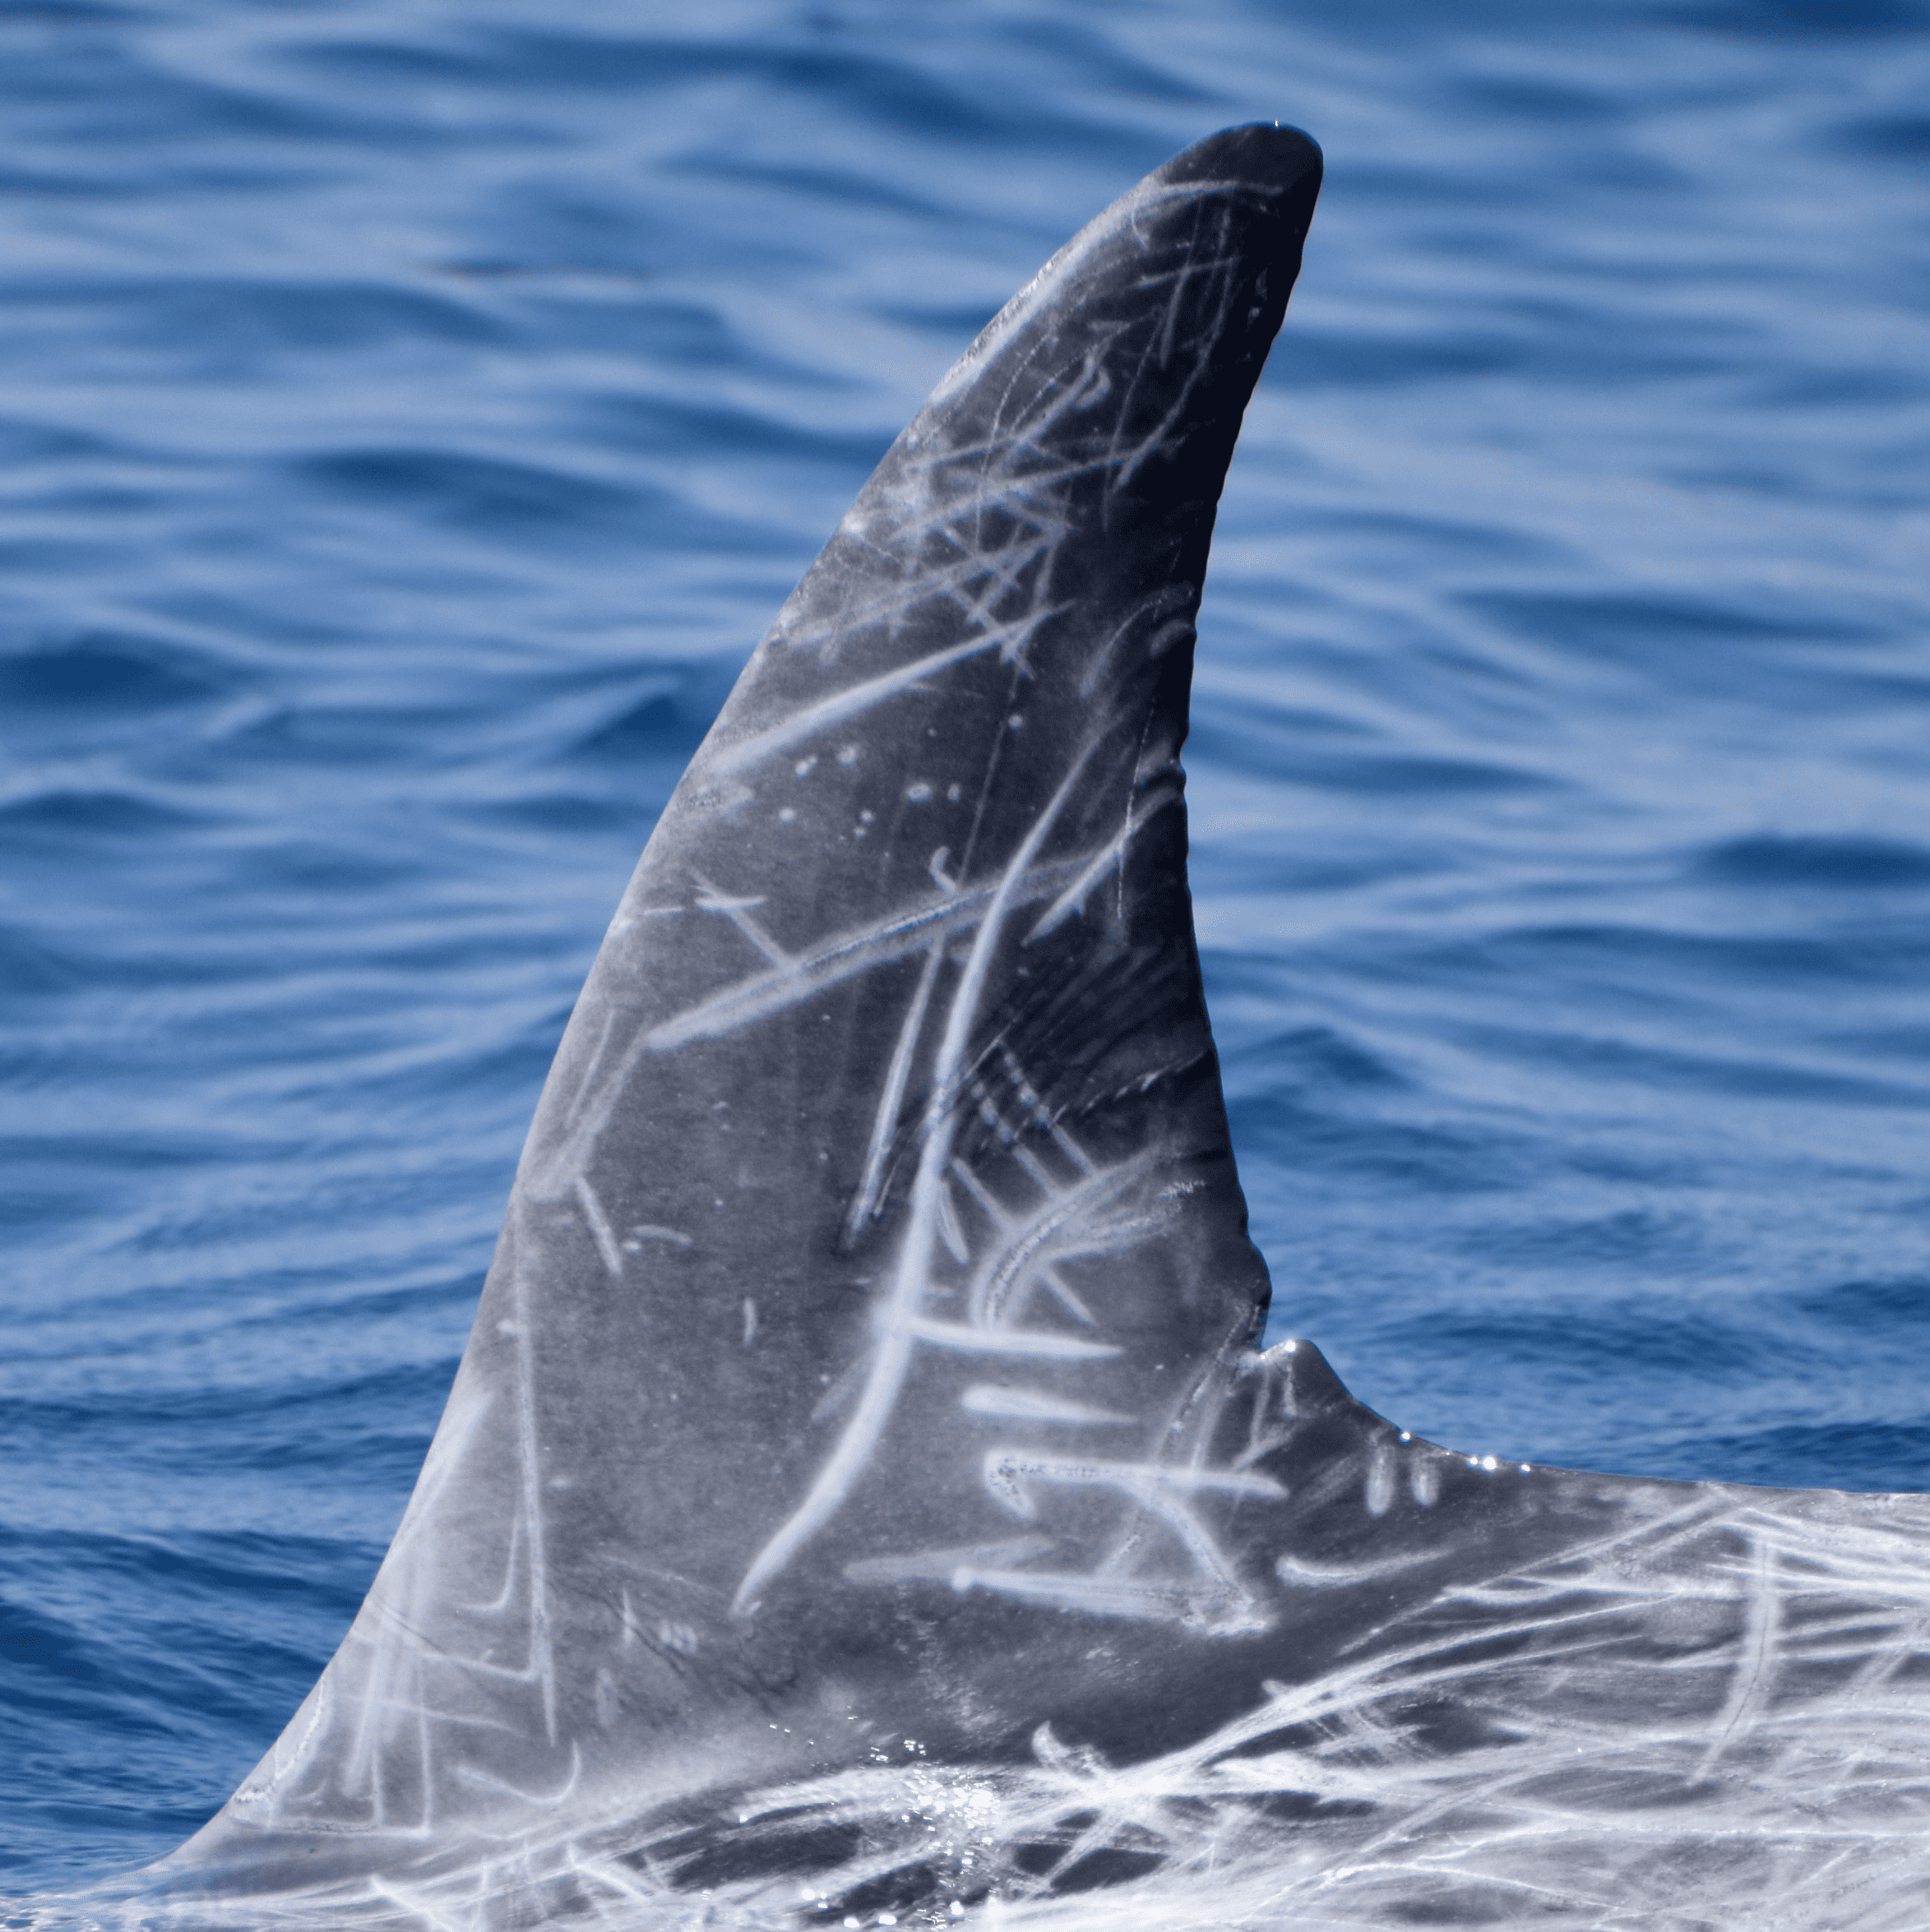
\includegraphics[width=\textwidth]{assets/images/methods/porting/fin_extraction/test_original.png}  
          \caption{Immagine originale}
        \end{minipage}
        \begin{minipage}{0.3\textwidth}
          \centering
          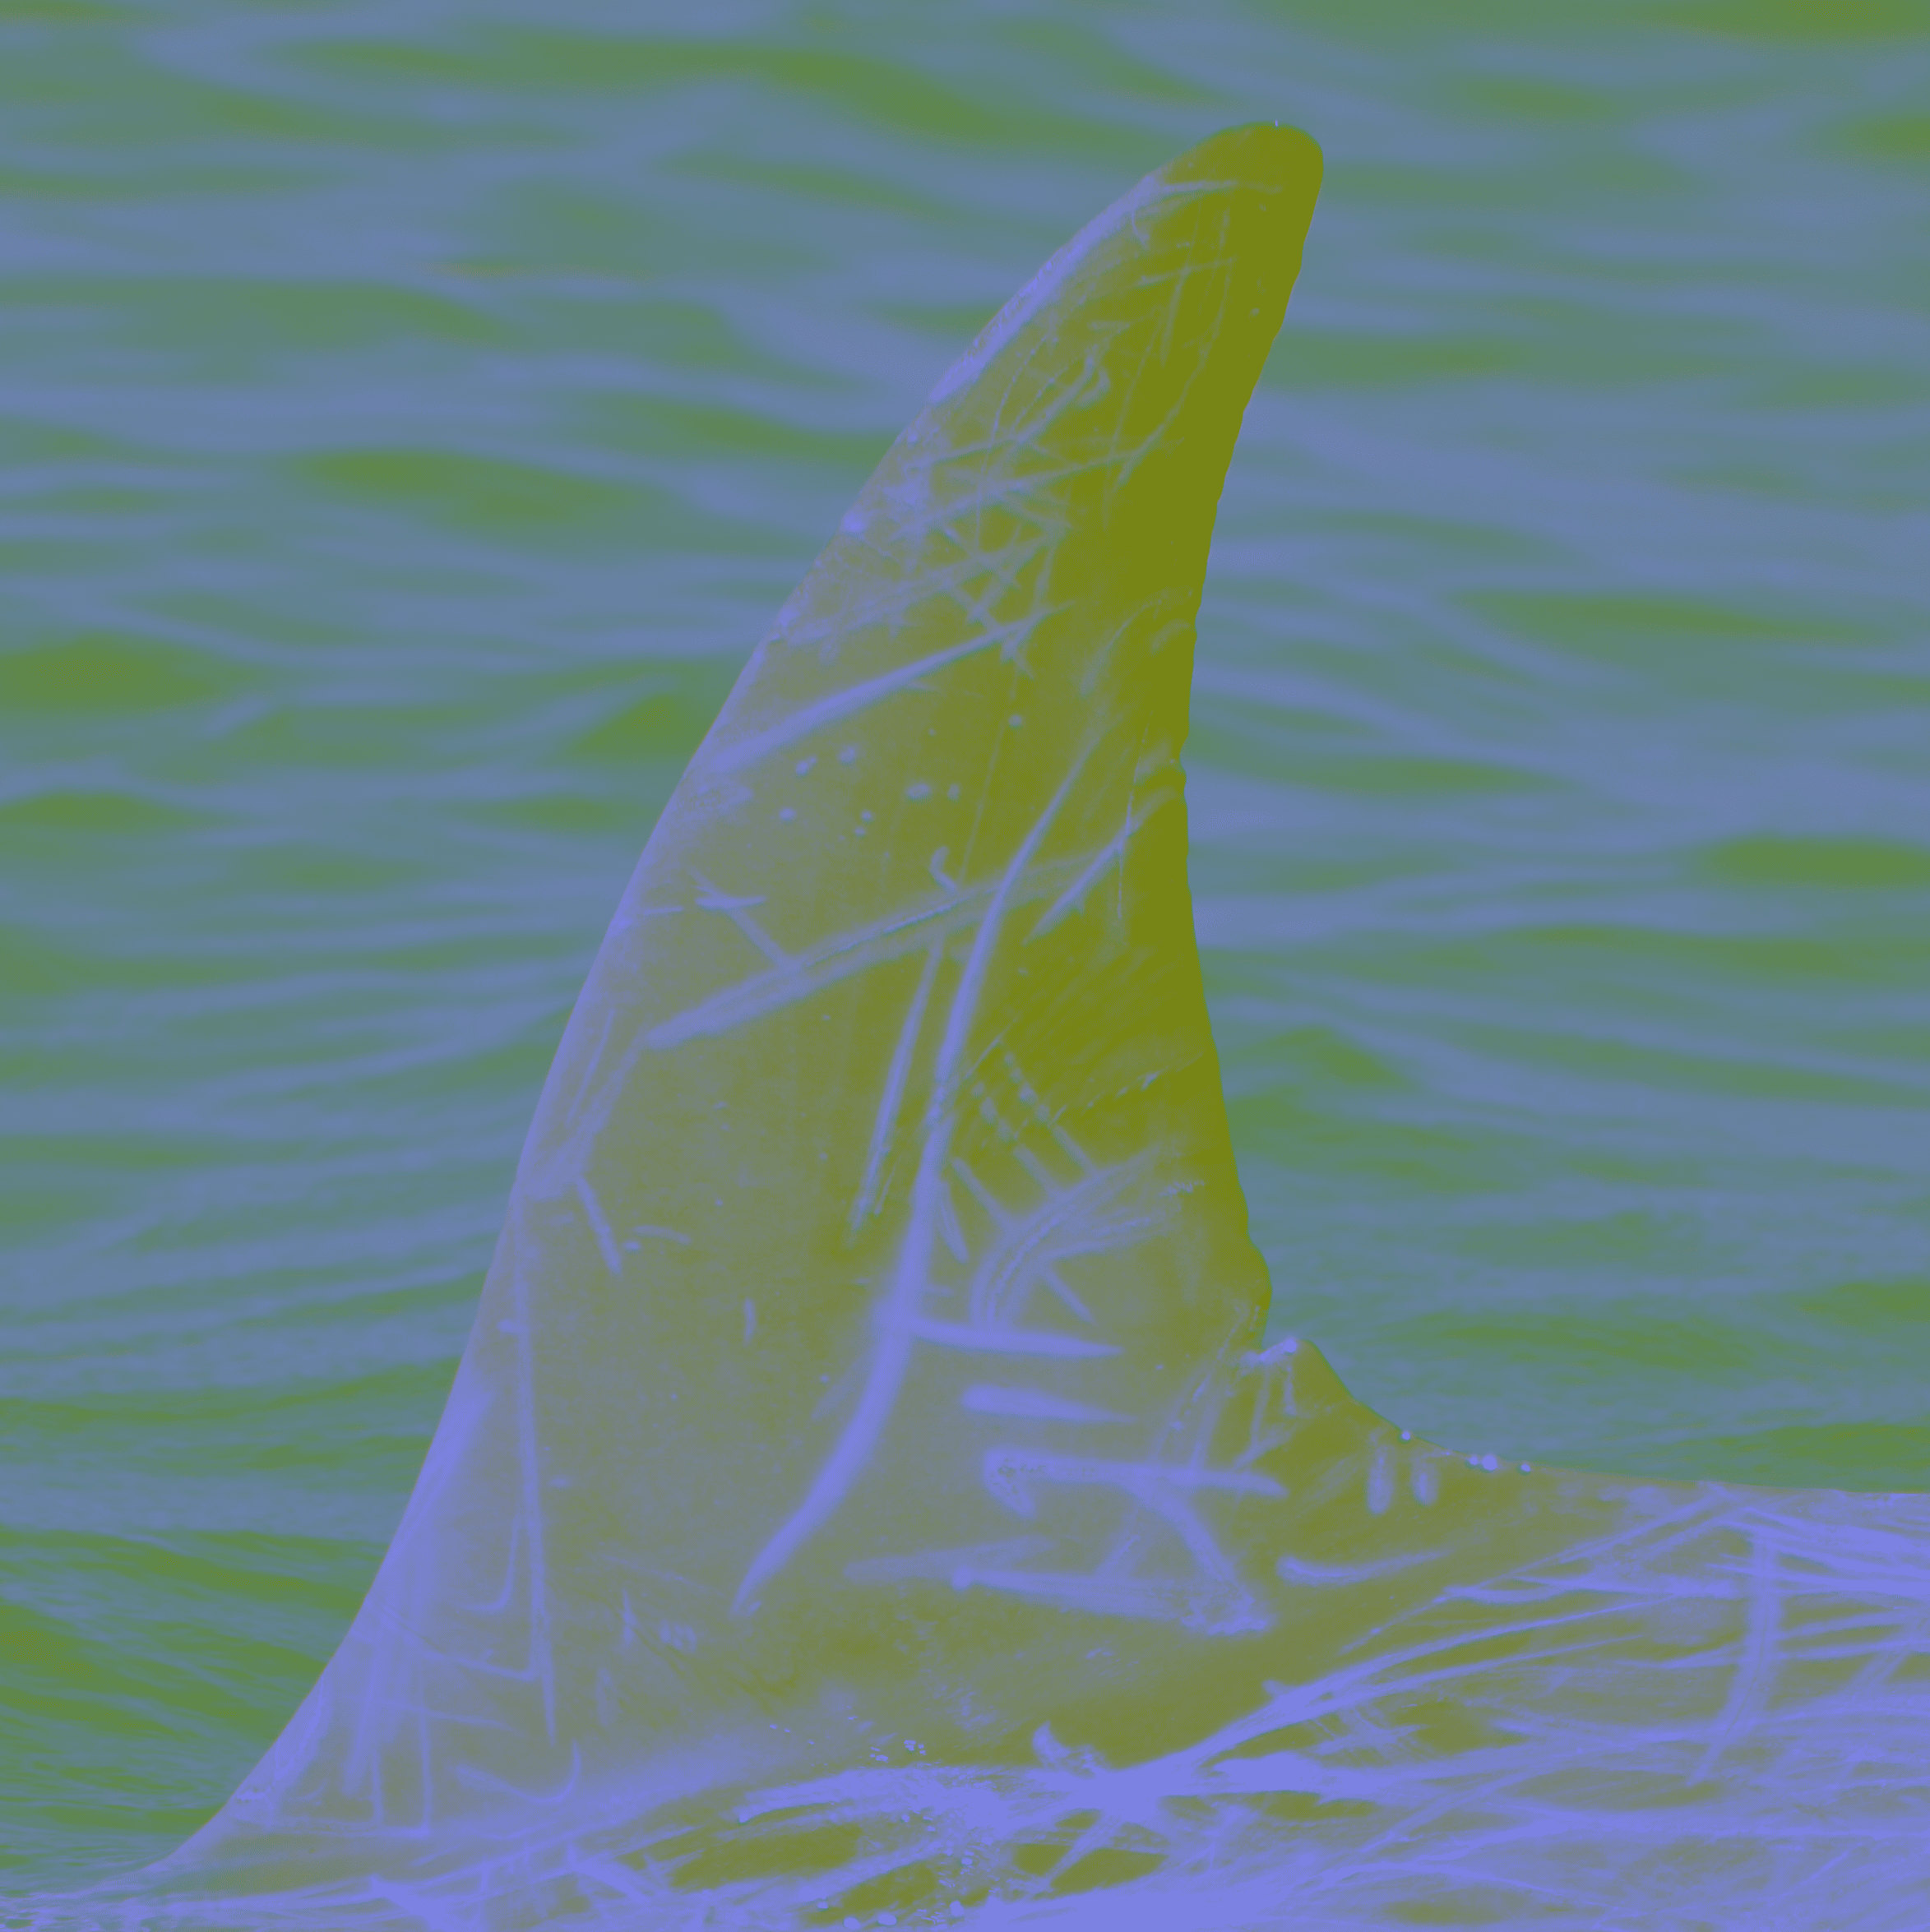
\includegraphics[width=\textwidth]{assets/images/methods/porting/fin_extraction/test_lab.png}   
          \caption{Immagine CIELAB}
        \end{minipage}
        \begin{minipage}{0.3\textwidth}
          \centering
          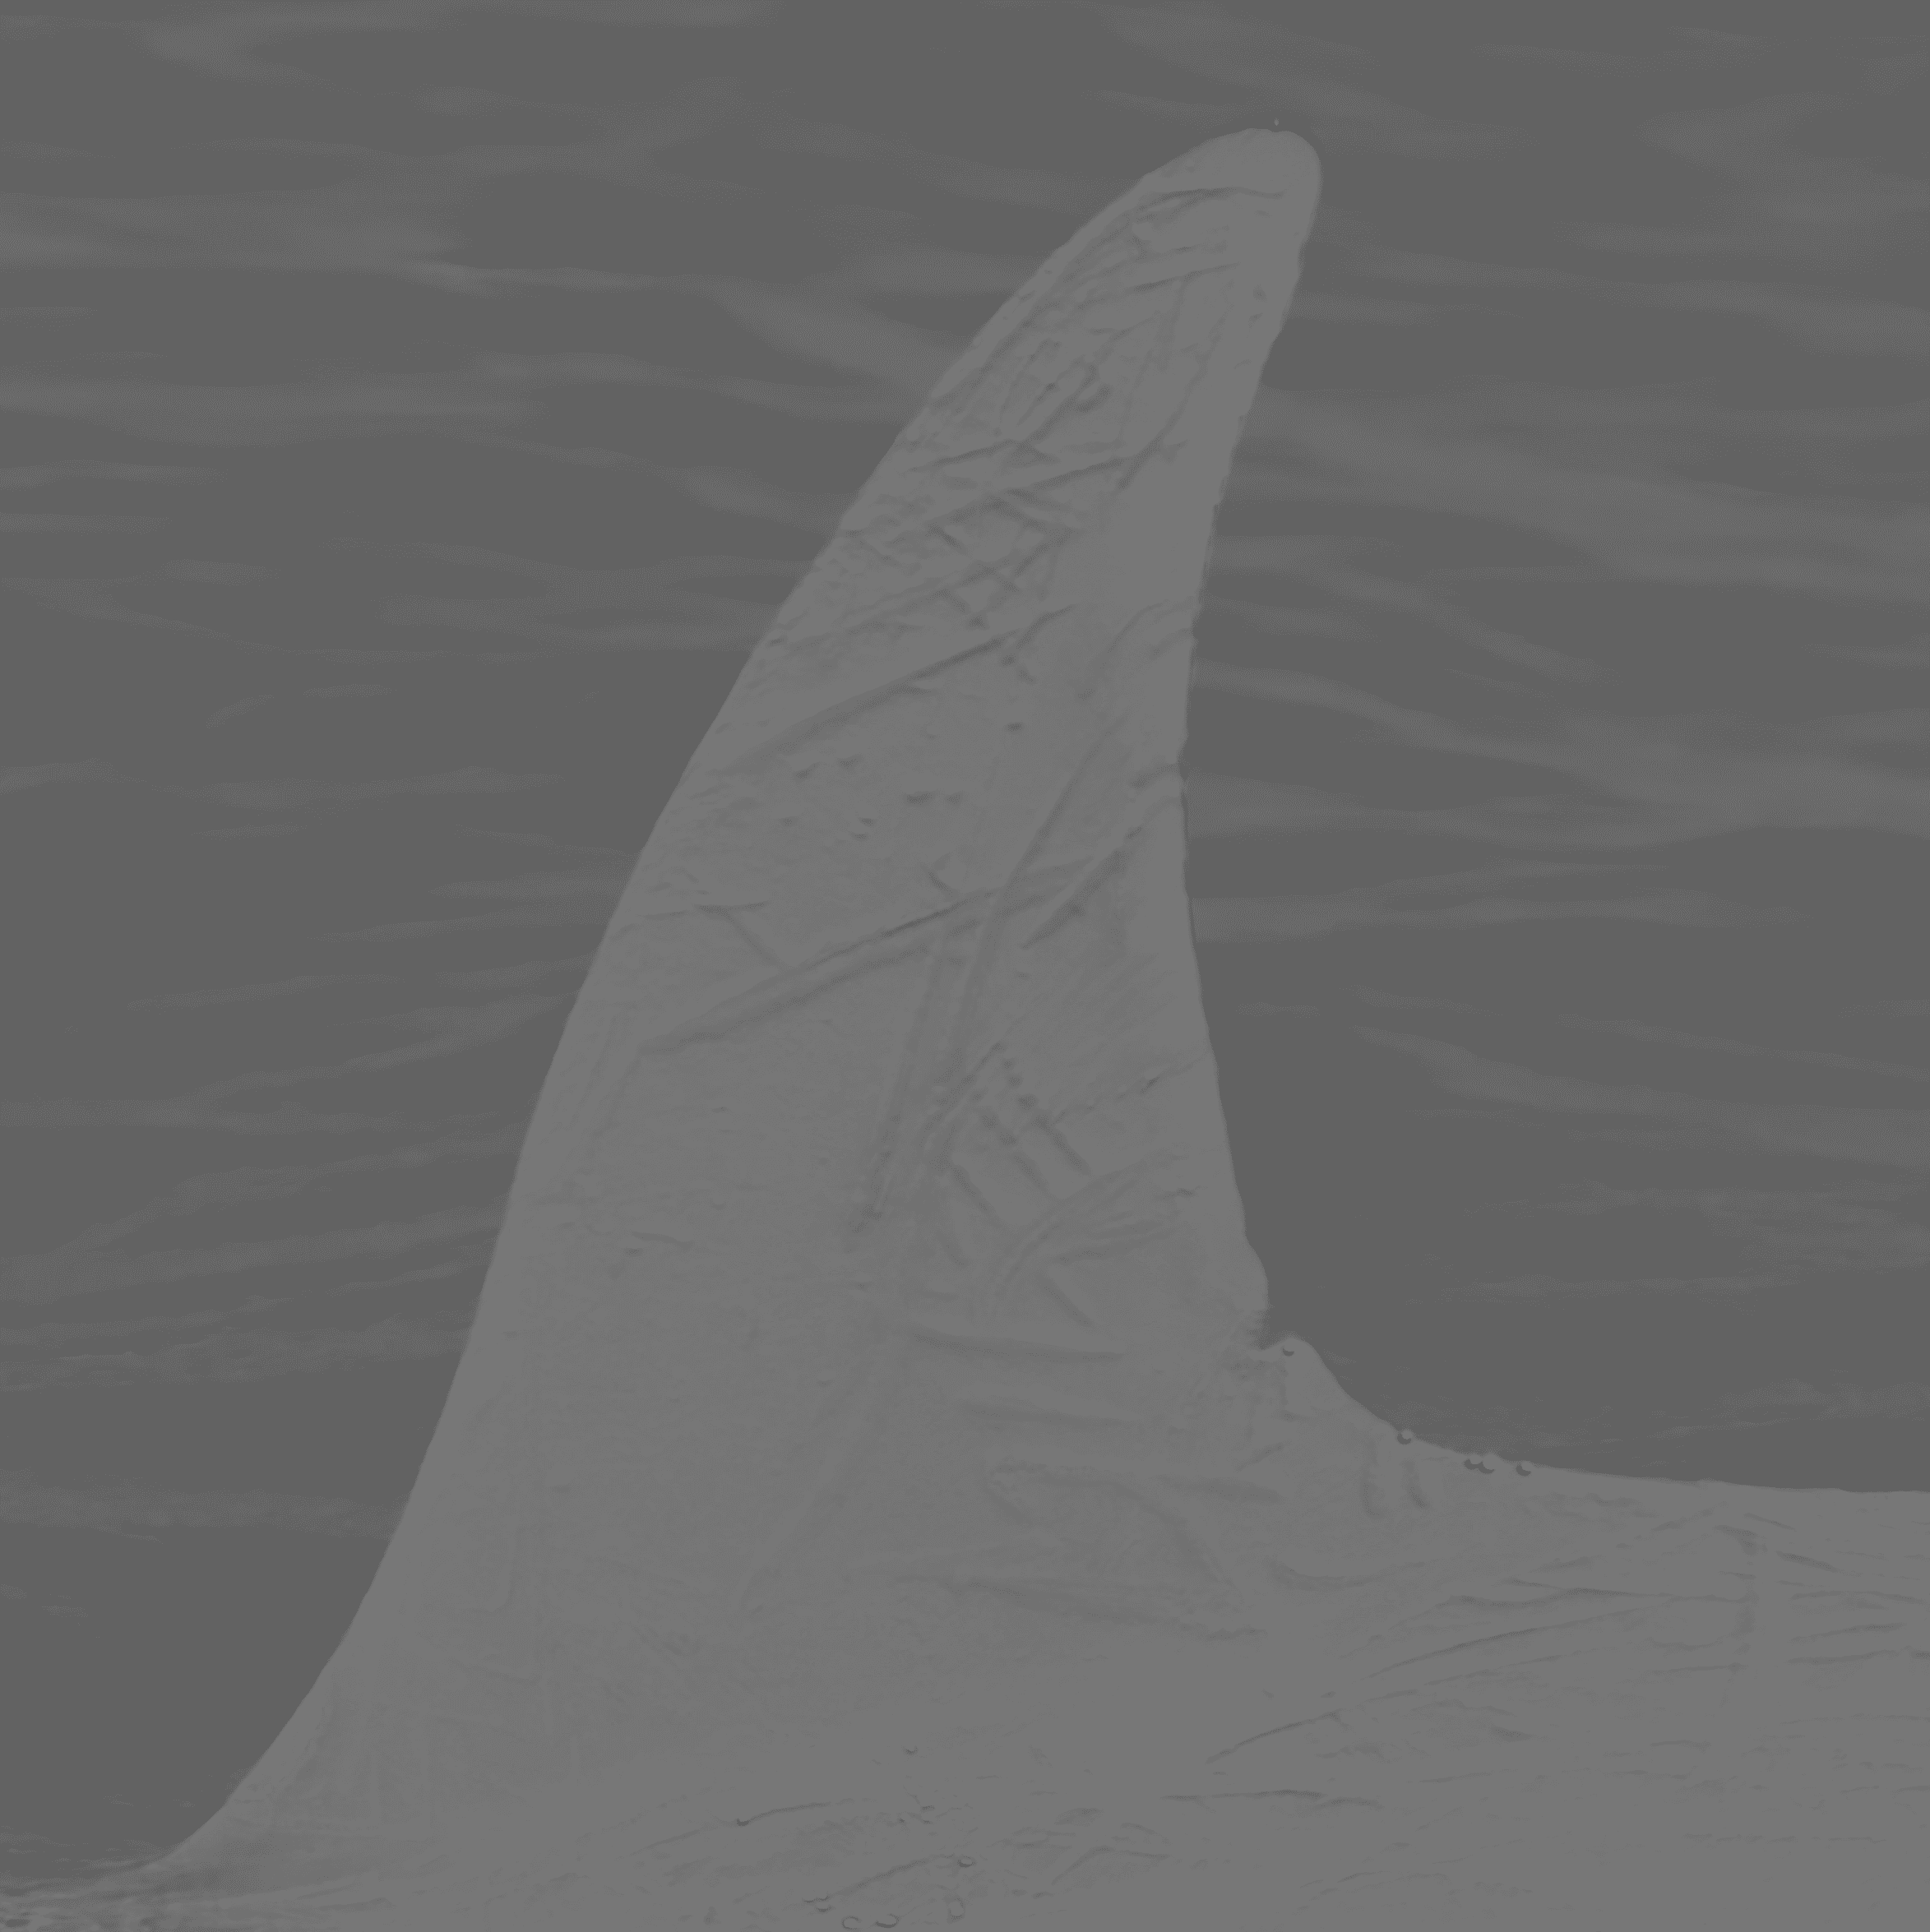
\includegraphics[width=\textwidth]{assets/images/methods/porting/fin_extraction/test_b.png}  
          \caption{Canale B estratto}
        \end{minipage}

        
      \end{figure}

\begin{lstlisting}
#Caricamento immagine originale
image = cv2.imread("BEN_180713_4.png")

#Conversione immagine in spazio colore CIELAB
im_lab = cv2.cvtColor(image, cv2.COLOR_BGR2LAB)

#Estrazione del canale B
b = im_lab[:,:,2]

# Applico il metodo di Otsu al canale B
thr_b, _ = cv2.threshold(b, 0, 255, cv2.THRESH_BINARY + cv2.THRESH_OTSU)
\end{lstlisting}
        L'algoritmo di Otsu \cite{otsu1979threshold} calcola la soglia ottimale in base all'istogramma dei livelli di grigio dell'immagine.
        L'istogramma rappresenta la distribuzione dei valori di grigio presenti nell'immagine.
        \newpage
        L'obiettivo è trovare la soglia che massimizza la varianza tra le due classi (primo piano e sfondo), 
        considerando anche la distribuzione dei pixel di ciascuna classe.
        In altre parole, si cerca la soglia che massimizza la separazione tra i due gruppi di pixel.

      \begin{figure}[H]
        \centering
        \begin{minipage}{0.3\textwidth}
          \centering
          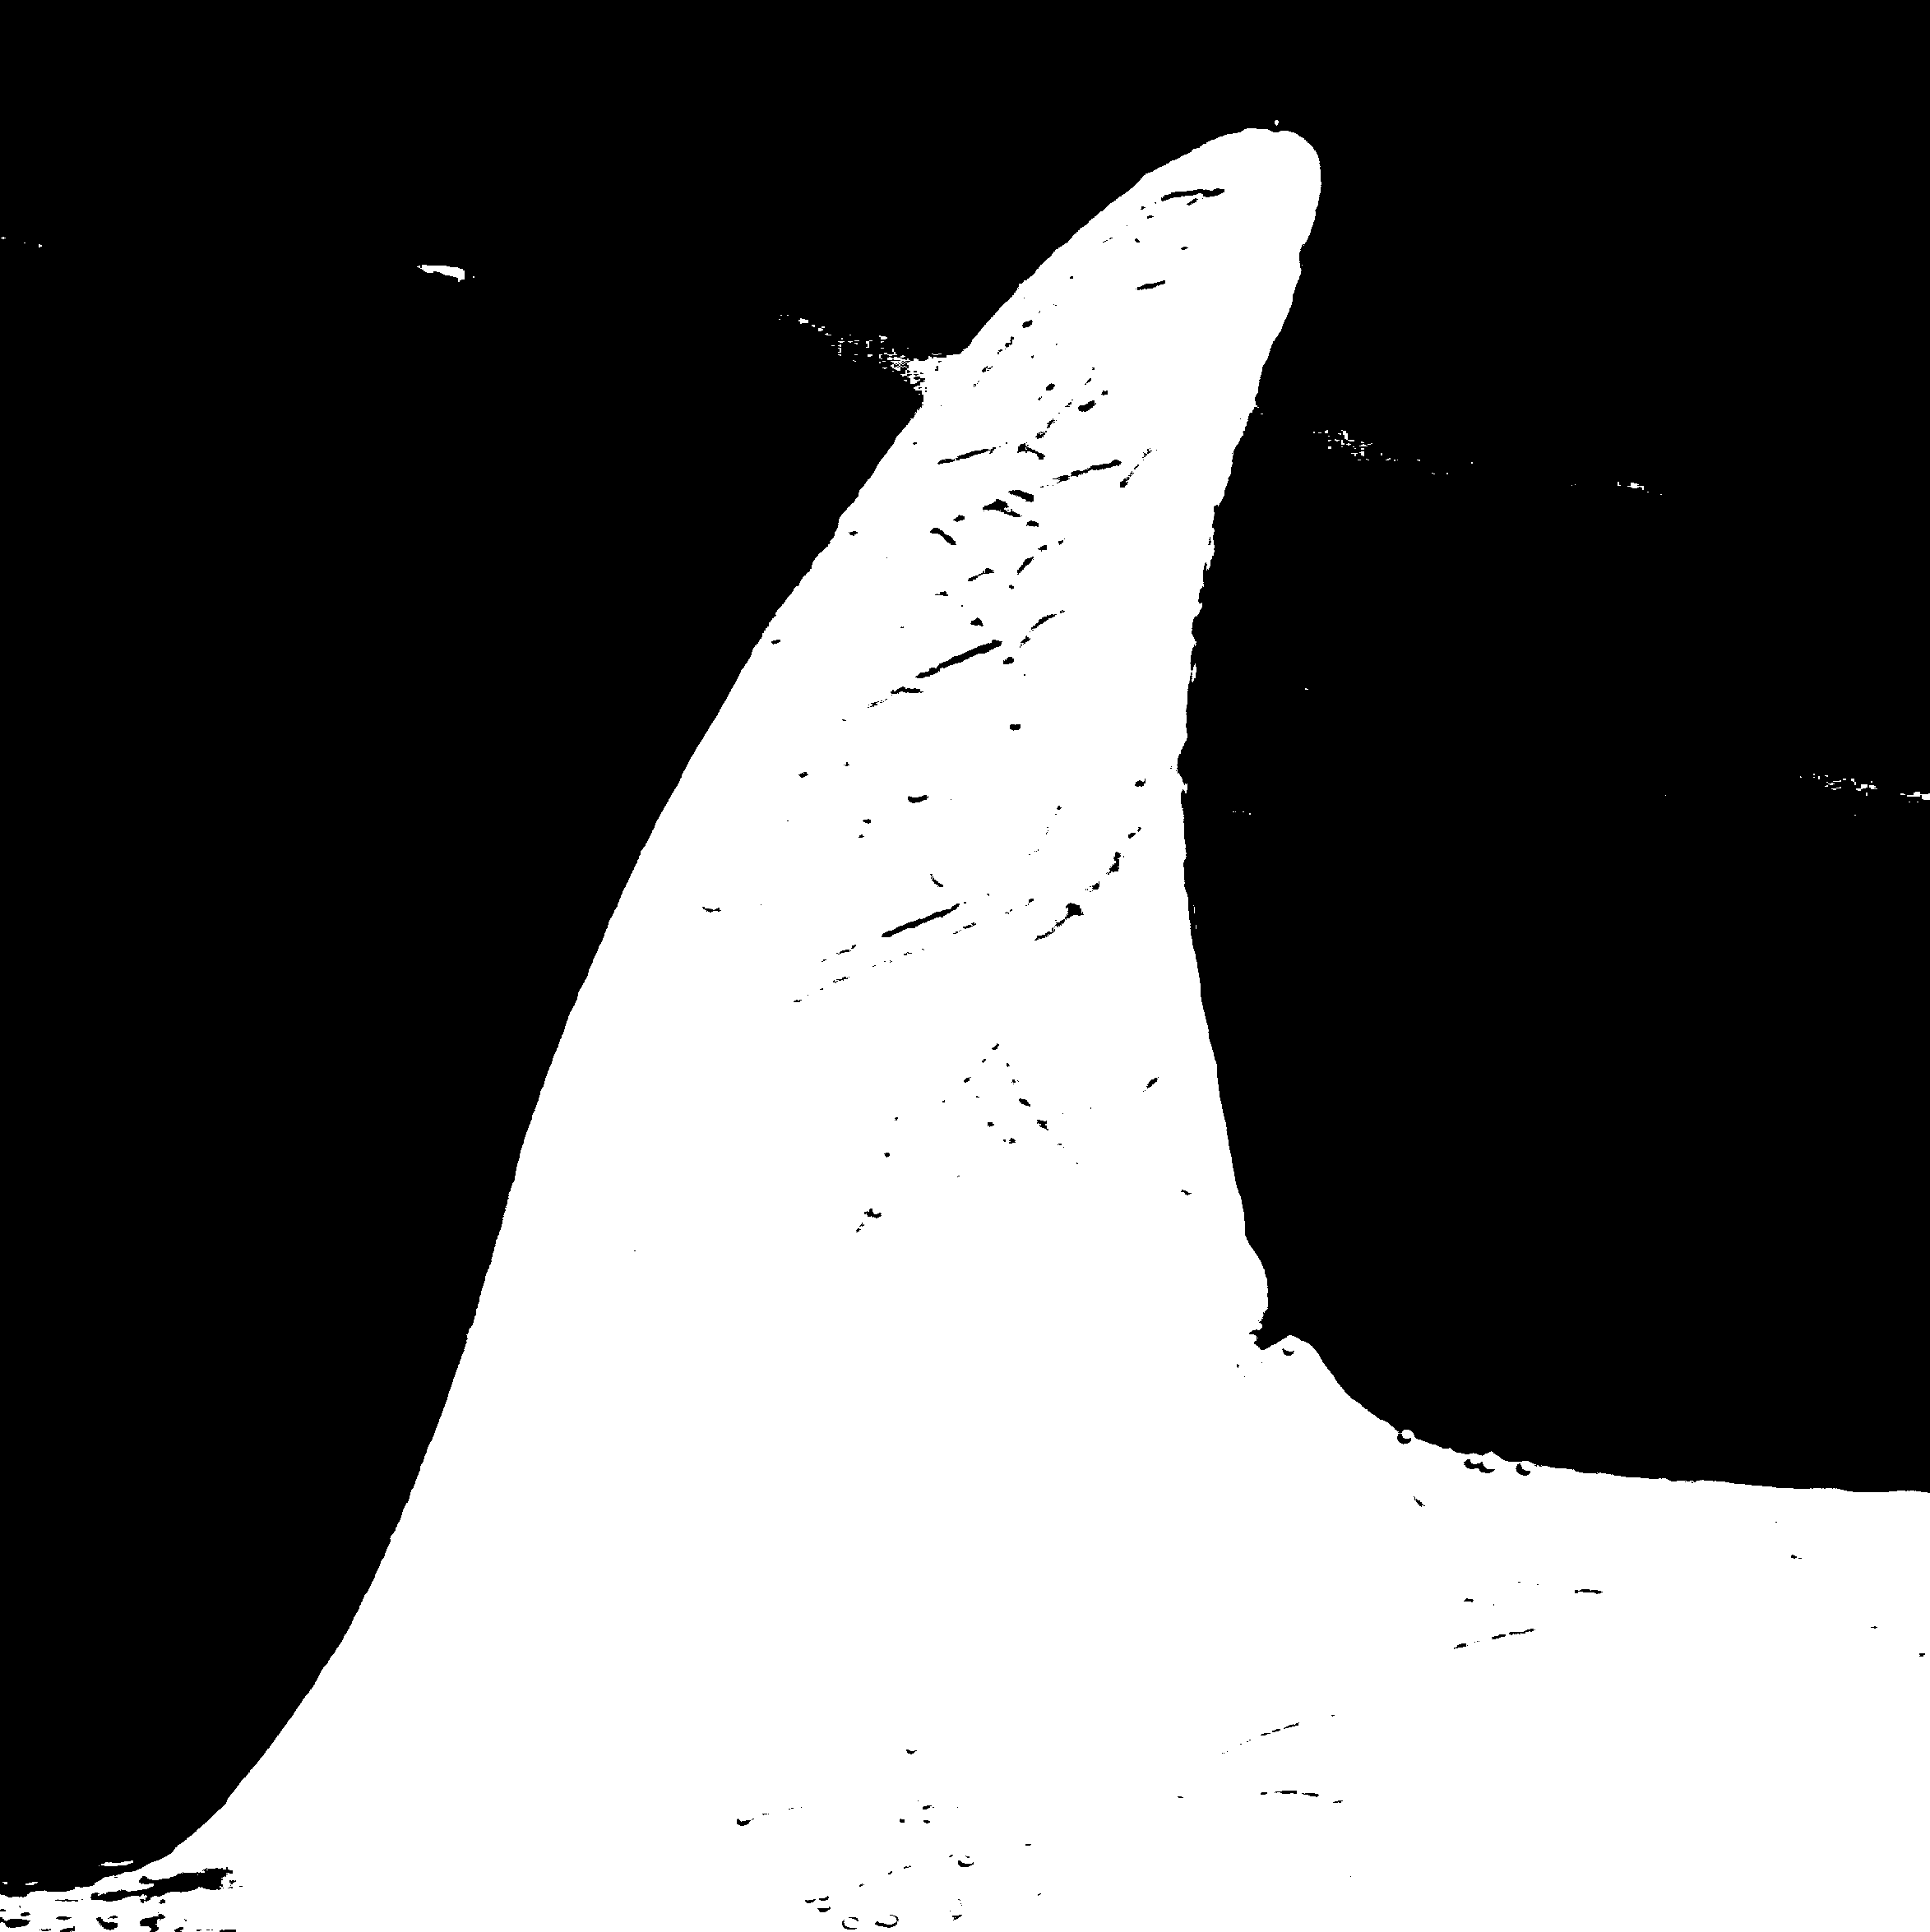
\includegraphics[width=\textwidth]{assets/images/methods/porting/fin_extraction/test_thr_b.png}   
          \caption{Metodo OTSU}
        \end{minipage}
        \begin{minipage}{0.3\textwidth}
          \centering
          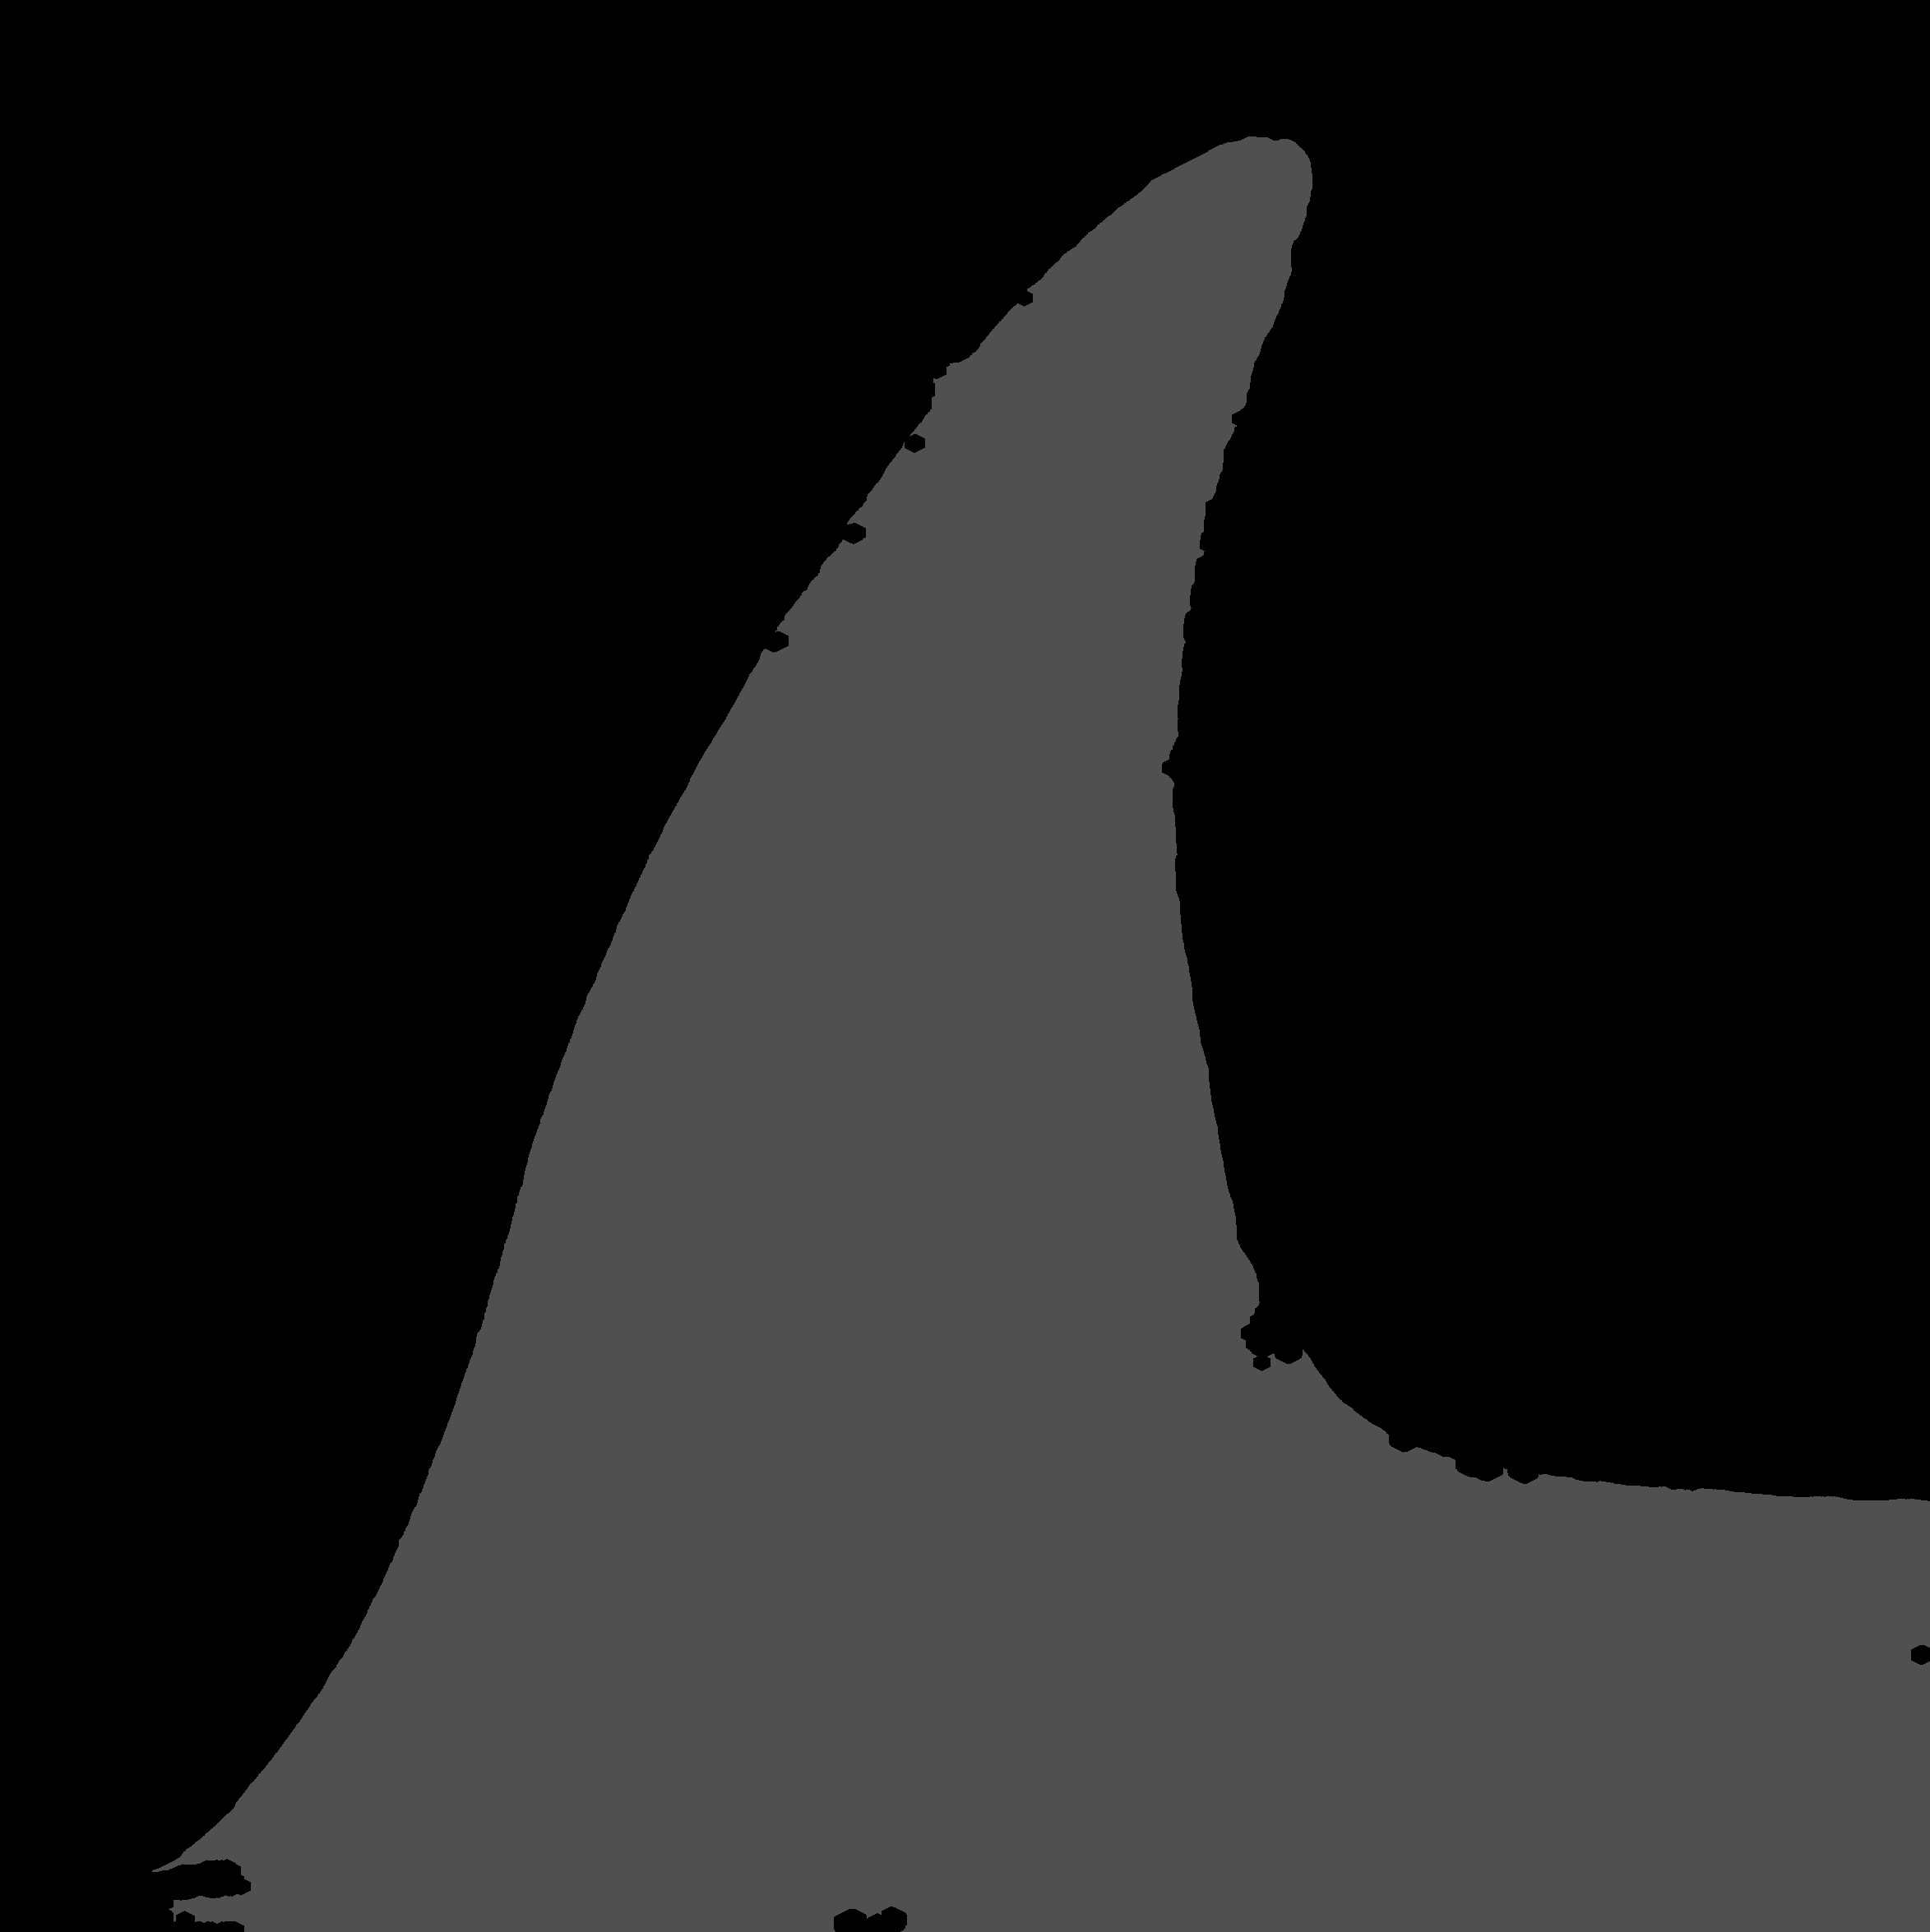
\includegraphics[width=\textwidth]{assets/images/methods/porting/fin_extraction/test_mask1.png}  
          \caption{Operatori morfologici e rimozione segmenti}
        \end{minipage}
        \begin{minipage}{0.3\textwidth}
          \centering
          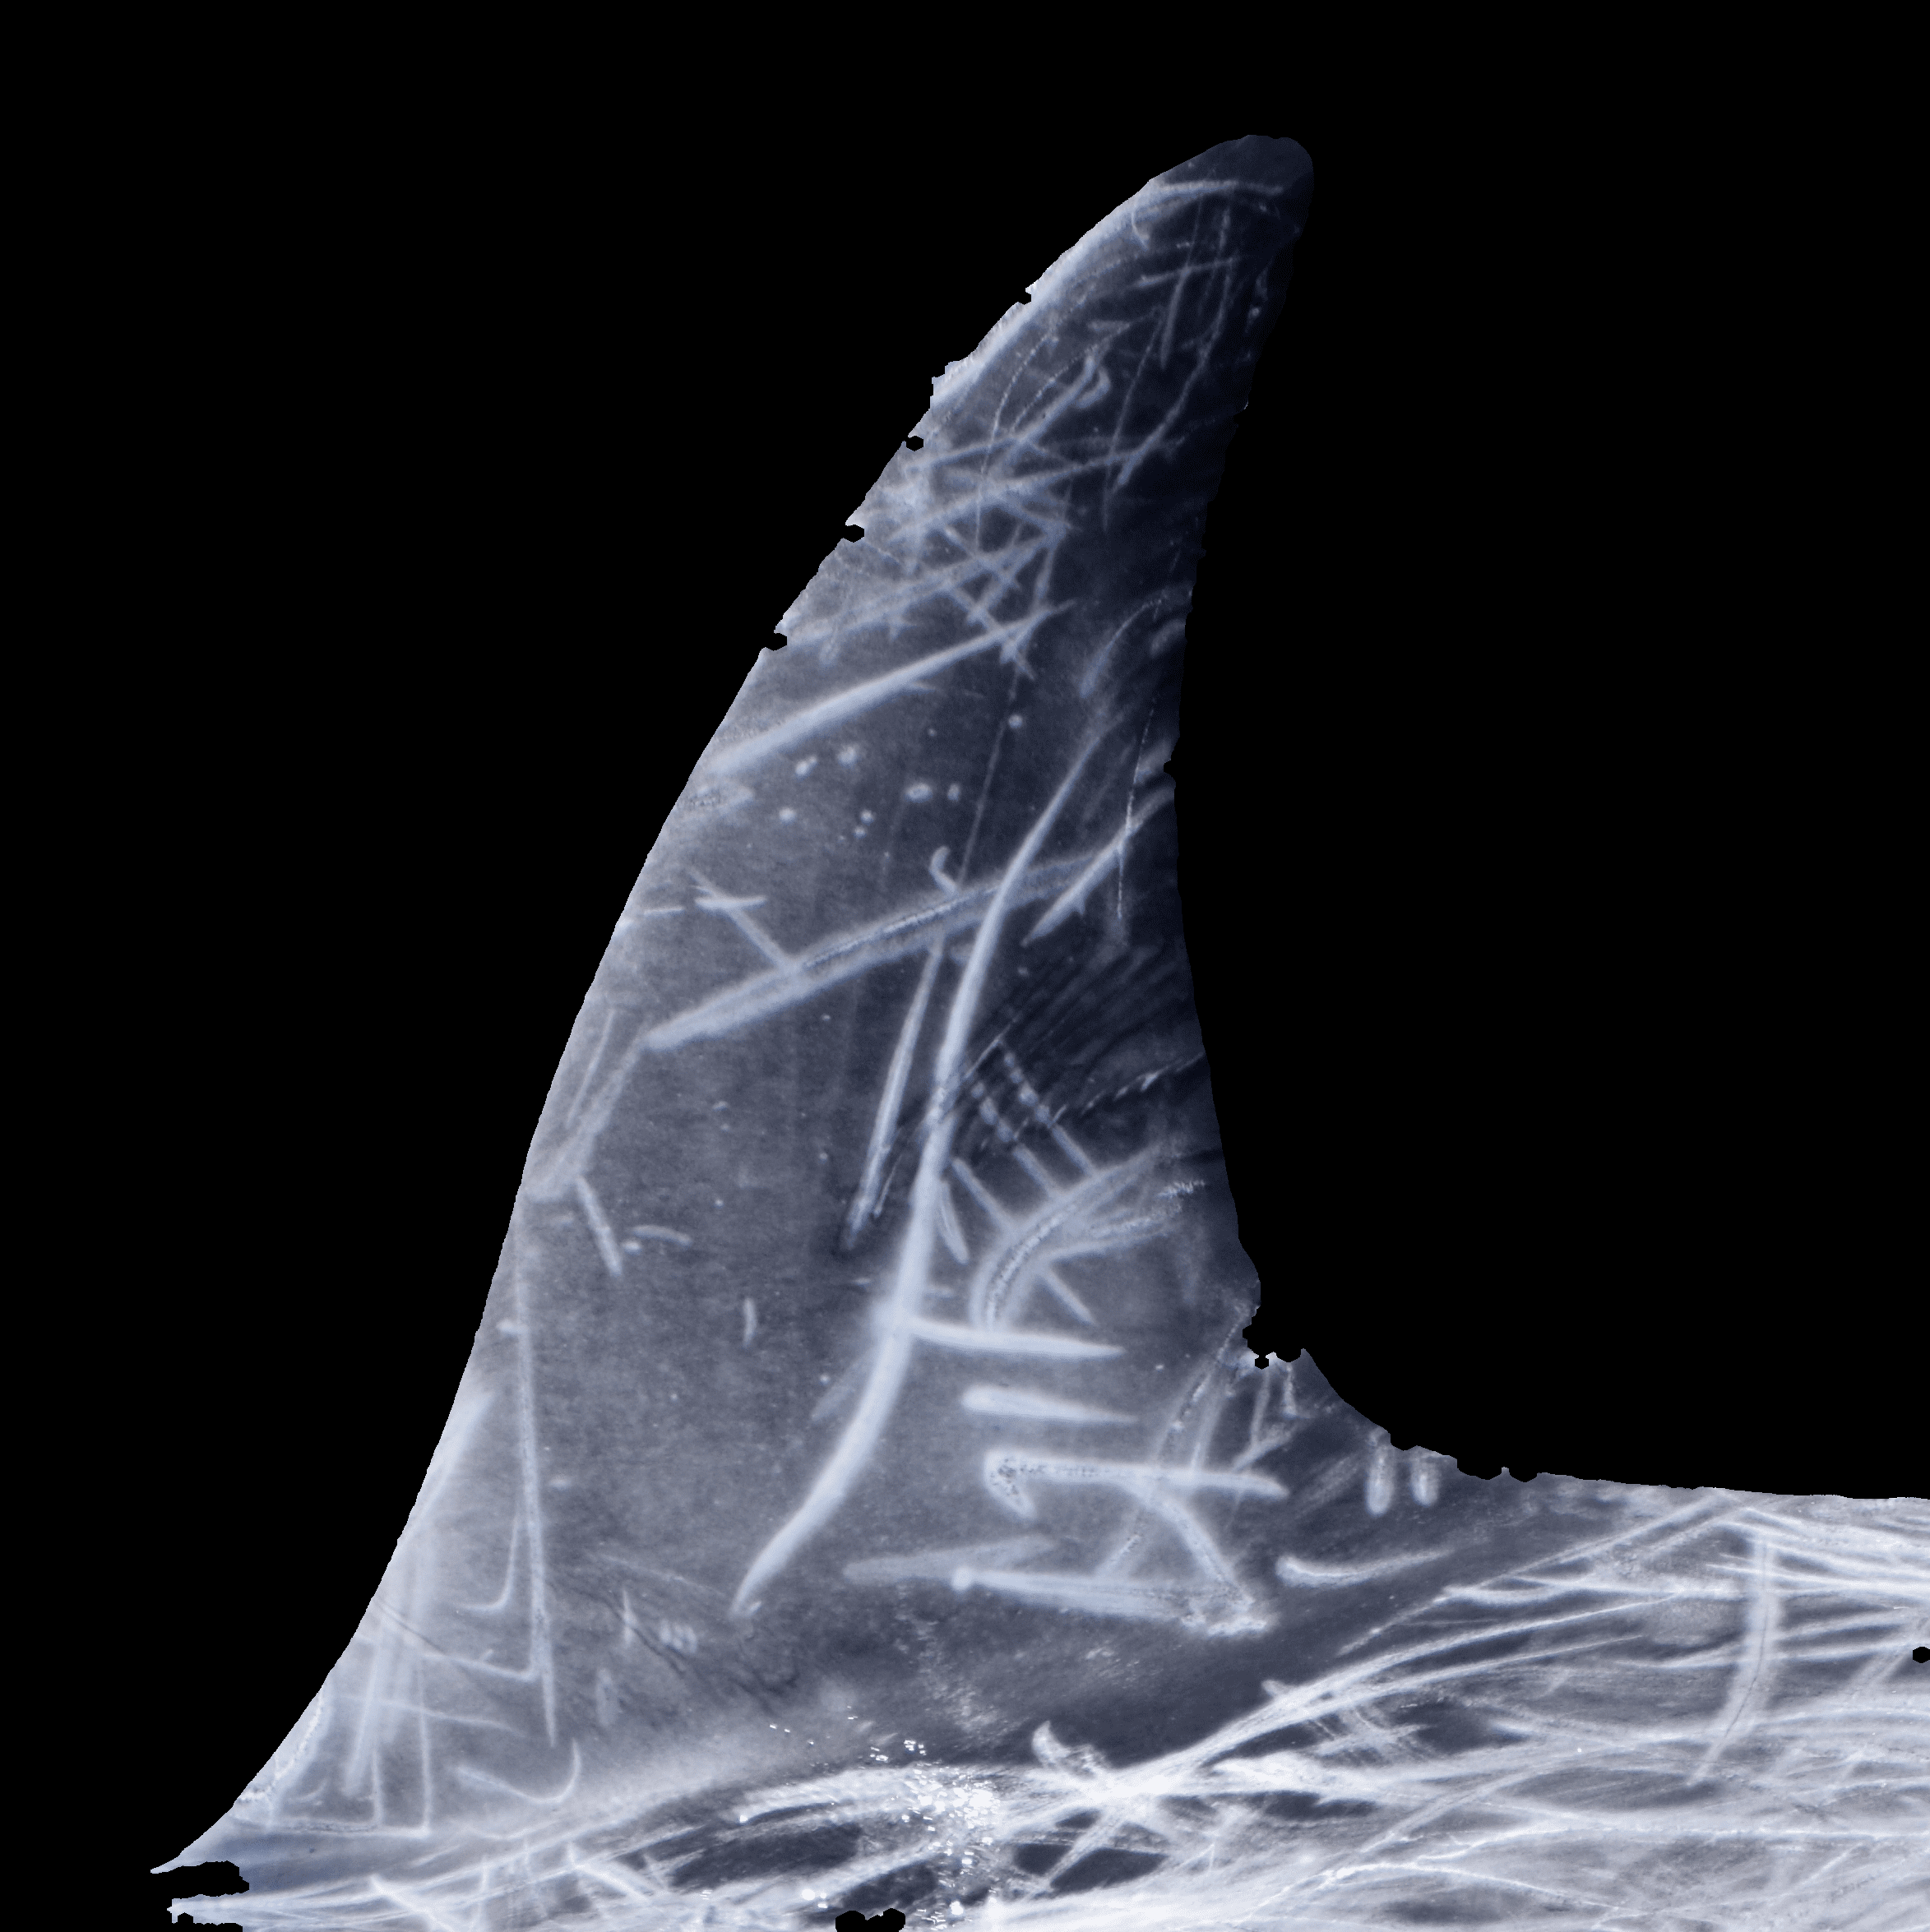
\includegraphics[width=\textwidth]{assets/images/methods/porting/fin_extraction/test_out.png}   
          \caption{Pinna estratta}
        \end{minipage}
        \begin{flushleft}
          
        \end{flushleft}
      \end{figure}
      Una volta prodotta la prima maschera grazie al metodo OTSU, 
      si passa all'eliminazione dei buchi mediante l'utilizzo di operatori
      morfologici e alla rimozione di segmenti slegati dall'area della pinna.
      Nello specifico gli operatori morfologici utilizzati per l'elimiazione dei buchi sono stati:
      \begin{itemize}
        \item Dilatazione (Dilation): L'operazione di dilatazione viene utilizzata per \\espandere le regioni di pixel bianchi nell'immagine. In sostanza, ogni pixel bianco nell'immagine di input viene "gonfiato" e riempito con pixel bianchi circostanti. Ciò ha l'effetto di aumentare le dimensioni dell'oggetto o delle strutture bianche nell'immagine. L'operazione di dilatazione è utile per riempire eventuali buchi o lacune all'interno delle regioni, connettere regioni separate o aumentare la dimensione degli oggetti.
        \newpage
        \item Chiusura (Closing): L'operazione di chiusura combina l'erosione seguita dalla dilatazione per rimuovere piccoli buchi o aree isolate all'interno delle regioni bianche dell'immagine. Inizialmente, l'operazione di erosione viene applicata per ridurre le dimensioni delle regioni bianche e rimuovere dettagli indesiderati. Successivamente, l'operazione di dilatazione viene applicata per riempire i buchi e ricongiungere le regioni vicine che potrebbero essere state separate durante l'erosione. L'operazione di chiusura è utile per ridurre il rumore, migliorare la coerenza delle regioni e completare le forme degli oggetti.
      \end{itemize}
      \begin{figure}[H]
        \centering
        \begin{minipage}{0.3\textwidth}
          \centering
          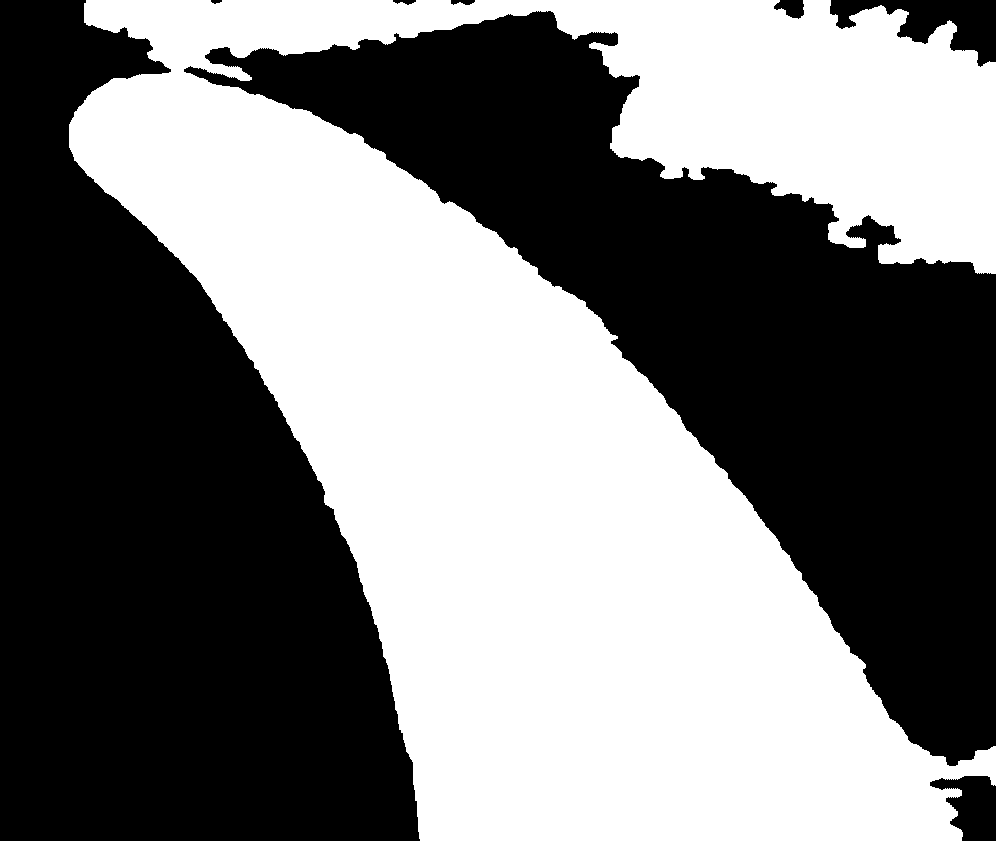
\includegraphics[width=\textwidth]{assets/images/methods/porting/alg_area/original.png}   
          \caption{Maschera originale}
        \end{minipage}
        \begin{minipage}{0.3\textwidth}
          \centering
          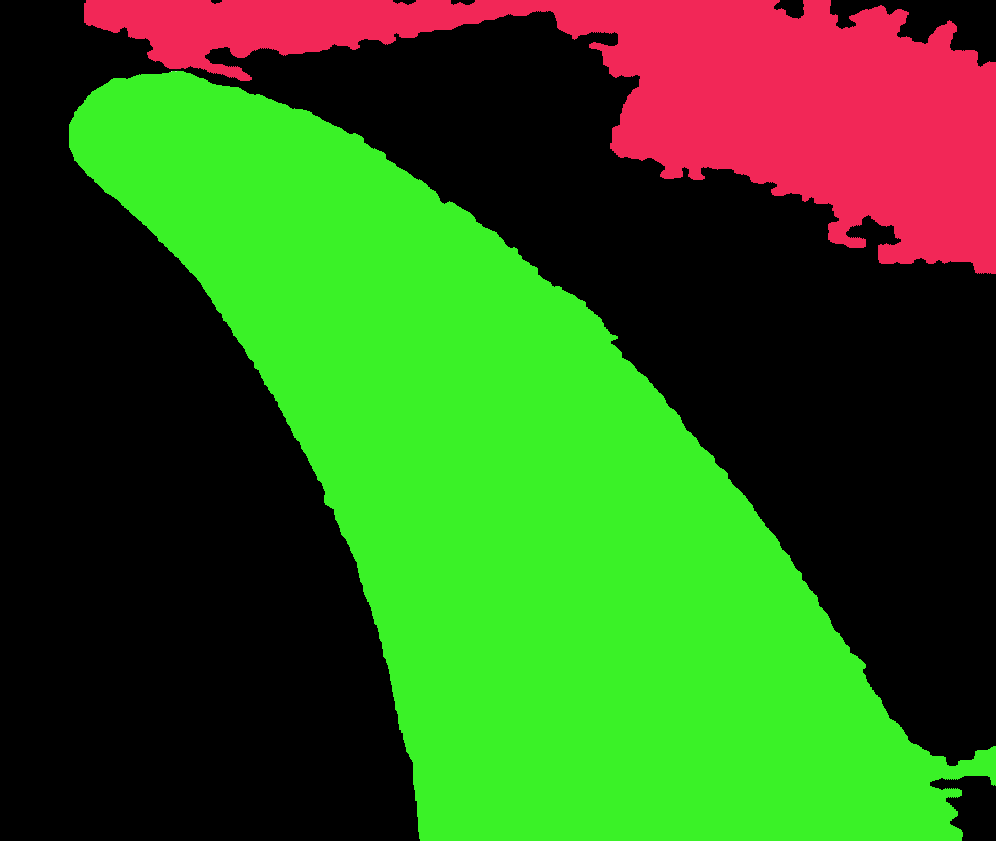
\includegraphics[width=\textwidth]{assets/images/methods/porting/alg_area/find.png}  
          \caption{Divisione in segmenti}
        \end{minipage}
        \begin{minipage}{0.3\textwidth}
          \centering
          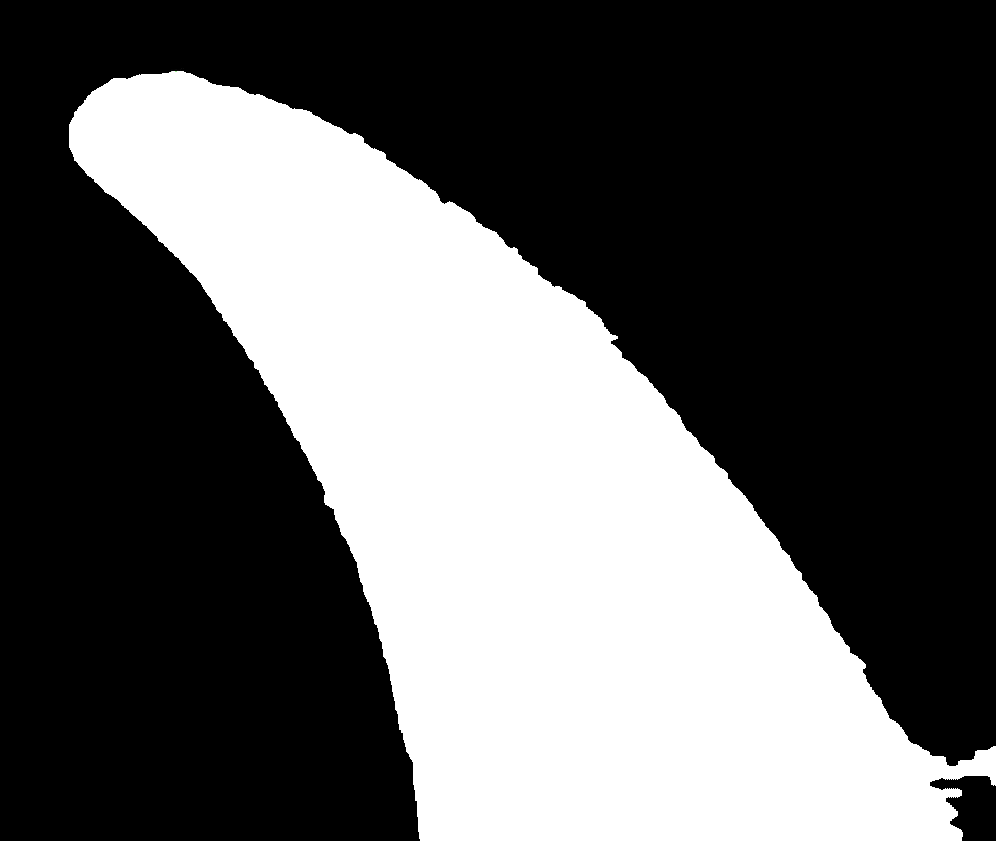
\includegraphics[width=\textwidth]{assets/images/methods/porting/alg_area/clear.png}   
          \caption{Rimozione segmenti minori}
        \end{minipage}
      \end{figure}
     
      Per quanto riguarda l'eliminazione di segmenti non appartenenti all'area della pinna del delfino
      è stato scritto un algoritmo che si basa sul trovare tutti i segmenti separati all'interno della maschera,
      cercare quello con l'area maggiore e poi rimuovere tutto il resto dalla maschera, 
      questa operazione viene ripetuta sia prima che dopo l'utilizzo degli operatori morfologici, con il fine di
      eliminare eventuali scarti dell'erosione o del metodo OTSU.
      \newpage

\begin{lstlisting}
#Trova i contorni nella maschera
contours, _ = cv2.findContours(im_thr, cv2.RETR_TREE, cv2.CHAIN_APPROX_NONE)

biggest_area = -1;
biggest = None;

for contour in contours:
    #Viene calcolata l'area del contorno
    area = cv2.contourArea(contour);

    #Salvataggio del contorno con l'area maggiore
    if biggest_area < area:
        biggest_area = area;
        biggest = contour;

#Disegno la maschera del contorno maggiore sulla maschera originale con una tonalità di grigio diversa
mask_colored = cv2.drawContours(im_thr, [biggest], -1, 80, -1);
_, binary_image = cv2.threshold(mask_colored, 254, 255, cv2.THRESH_BINARY_INV)

#Estraggo la maschera del contorno maggiore
mask = cv2.bitwise_and(mask_colored, mask_colored, mask=binary_image)

kernel = cv2.getStructuringElement(cv2.MORPH_ELLIPSE, (5,5))

#Applico operatori morfologici per eliminare eventuali buchi nella maschera
mask = cv2.morphologyEx(mask, cv2.MORPH_DILATE, kernel=kernel, iterations=1)
mask = cv2.morphologyEx(mask, cv2.MORPH_CLOSE, kernel=kernel, iterations=1)

#Altra Rimozione dei segmenti
#...
#Applico la maschera all'immagine originale per estrarre la pinna
fin = cv2.bitwise_and(image, image, mask=mask)
\end{lstlisting}
    \subsection{Controllo qualità}
    \begin{figure}[H]
      \centering
      \begin{minipage}{0.3\textwidth}
        \centering
        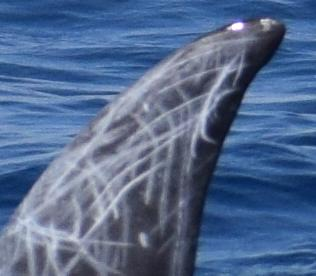
\includegraphics[width=\textwidth]{assets/images/methods/porting/quality_control/blur.png}  
        \caption{Foto sfocata (Blur)}
      \end{minipage}
      \begin{minipage}{0.3\textwidth}
        \centering
        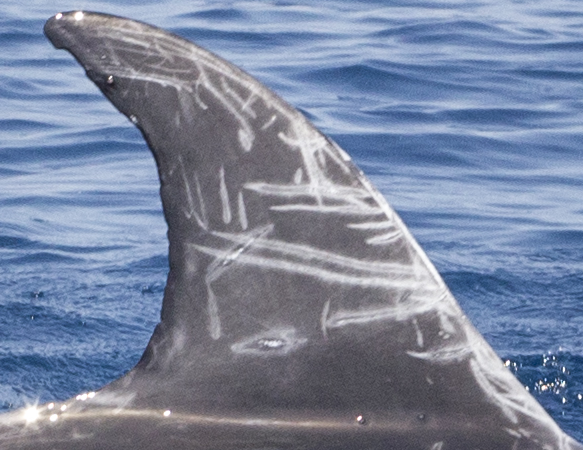
\includegraphics[width=\textwidth]{assets/images/methods/porting/quality_control/contrast.png}   
        \caption{Foto con basso contrasto (Contrast)}
      \end{minipage}
      \begin{minipage}{0.3\textwidth}
        \centering
        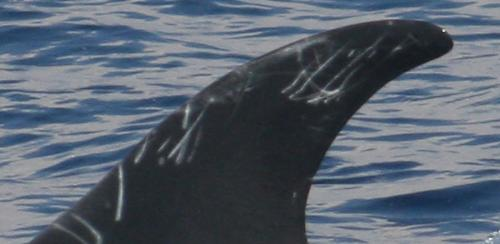
\includegraphics[width=\textwidth]{assets/images/methods/porting/quality_control/snr.png}   
        \caption{Foto con rumore (SNR)}
      \end{minipage}
    \end{figure}
    Una prima fase di filtraggio delle immagini viene applicata utilizzando dei metodi di 
    controllo della qualità delle immagini, questo con il fine di scartare le foto con caratteristiche 
    che andrebbero a compromettere a priori la fase di estrazione della maschera, data la scarsa qualità,
    per effettuare questo controllo di utilizzano le seguenti metriche:
    \begin{itemize}
      \item Blur (sfocatura): La sfocatura si riferisce alla mancanza di nitidezza o di dettaglio nell'immagine. Misurare il livello di sfocatura è importante per valutare la qualità e la definizione di un'immagine. La sfocatura può essere causata da vari fattori come l'acquisizione non precisa dell'immagine, il movimento della fotocamera durante lo scatto o la compressione dell'immagine. La metrica di blur viene utilizzata per quantificare il grado di sfocatura presente nell'immagine e può aiutare a determinare se l'immagine soddisfa i requisiti desiderati in termini di nitidezza.
      \begin{lstlisting}
#Calcola la sfocatura utlizzando
#il filtro Laplaciano
blur = cv2.Laplacian(fin_gray, cv2.CV_64F).var()
      \end{lstlisting}
   
      \newpage
      \item Contrast (contrasto): Il contrasto si riferisce alla differenza di luminosità tra le diverse parti di un'immagine. Un buon contrasto è importante perché consente di distinguere meglio gli oggetti e i dettagli presenti nell'immagine. La metrica di contrasto valuta la differenza di intensità tra le regioni chiare e quelle scure dell'immagine. Un contrasto adeguato può migliorare la leggibilità e l'interpretazione dell'immagine stessa.
      \begin{lstlisting}
#Calcola il contrasto 
#utilizzando la deviazione standard
contrast = np.std(fin_gray)
      \end{lstlisting}
      \item SNR (Signal-to-Noise Ratio) o rapporto segnale-rumore: L'SNR è una misura che indica il livello del segnale rispetto al rumore presente in un'immagine. Il rumore può essere causato da vari fattori come l'acquisizione dell'immagine con condizioni di illuminazione scarsa, l'interferenza elettrica o il rumore introdotto durante la trasmissione o la compressione dell'immagine. Un alto rapporto segnale-rumore indica che il segnale (informazione utile) è predominante rispetto al rumore indesiderato nell'immagine. L'SNR è una metrica importante per valutare la qualità e la fedeltà dell'immagine, in quanto un alto SNR indica una migliore qualità dell'immagine in termini di dettaglio e fedeltà visiva.
      \begin{lstlisting}
signal_energy = np.sum(fin_gray ** 2)
noise_energy = np.sum((fin_gray - cv2.GaussianBlur(fin_gray, (5, 5), 0)) ** 2)
snr = 10 * np.log10(signal_energy / noise_energy)
      \end{lstlisting}
    \end{itemize}


    \begin{figure}[H]
      \centering
      \begin{minipage}{0.4\textwidth}
        \centering
        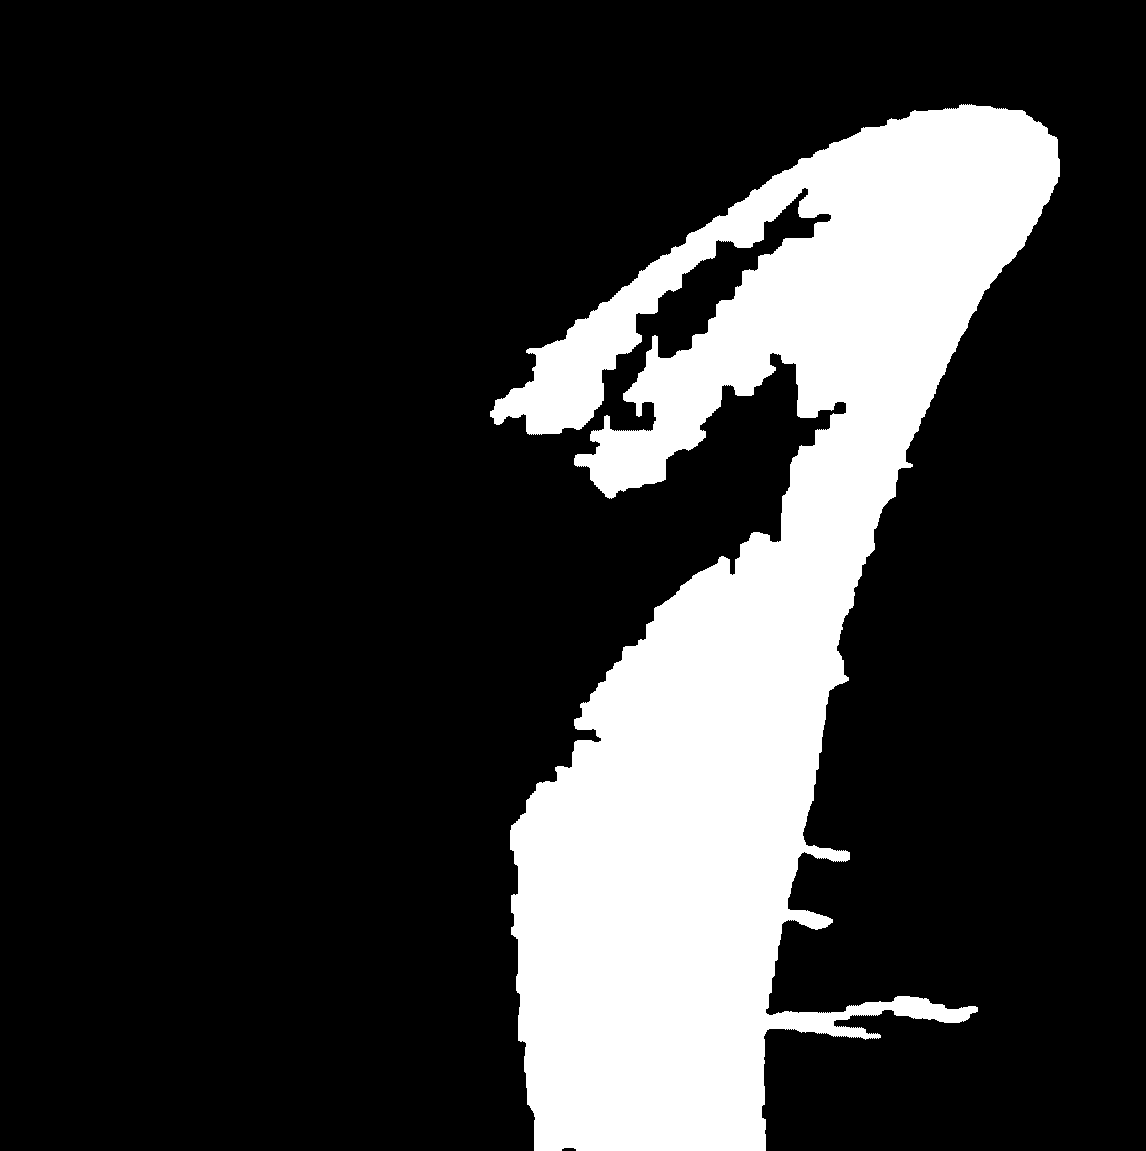
\includegraphics[width=\textwidth]{assets/images/methods/porting/quality_control/less.png}  
        \caption{\\$finArea < minFinArea$}
      \end{minipage}
      \begin{minipage}{0.4\textwidth}
        \centering
        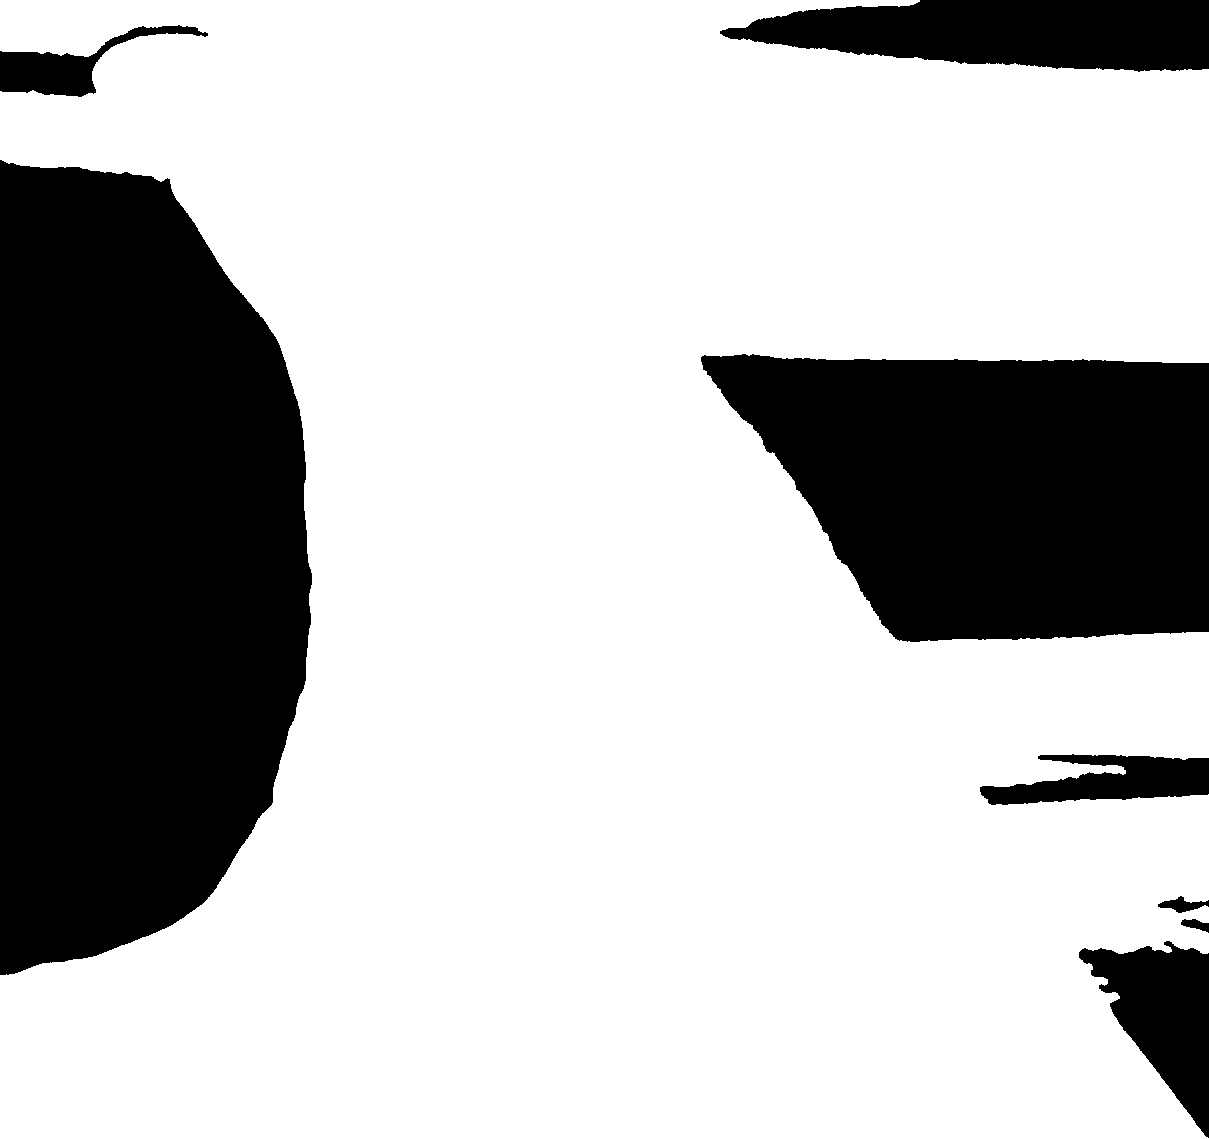
\includegraphics[width=\textwidth]{assets/images/methods/porting/quality_control/too.png}   
        \caption{\\$maxFinArea < finArea$}
      \end{minipage}
    \end{figure}
    
    Per migliorare la qualità complessiva delle maschere estratte da passare alla fase di feature extraction,
    si sceglie di porre diversi livelli di filtraggio con relativi parametri soglia.
    Un secondo controllo viene dunque effettuato sulla maschera generata. Se 
    dopo tutti i passaggi di ottimizzazione della maschera (compresa l'eliminazione di
    segmenti), l'area della maschera non rispetta la seguente disequazione:
    \begin{minipage}{1\textwidth}
      \centering
      $minFinArea \leq finArea \leq maxFinArea$
    \end{minipage}
    
    allora l'immagine sarà scartata, dato che sicuramente l'estrazione della maschera
    non avrà correttamente segmentato la pinna del delfino, sia in caso di eccesso o assenza di area.
    
    \begin{lstlisting}
min_fin_area = 33, max_fin_area = 66
mask_pixels = np.sum(mask == 255)
total_pixels = mask.shape[0] * mask.shape[1]
fin_area = (mask_pixels / total_pixels)*100
# ...
if fin_area < min_fin_area or fin_area > max_fin_area:
  model.state = ModelData.ERR_AREA
  return model

model.state = ModelData.OK
return model
    \end{lstlisting}
    \newpage
   
    \subsection{Estrazione delle features}
    \begin{figure}[H]
      
      \centering
      \begin{minipage}{0.3\textwidth}
        \centering
        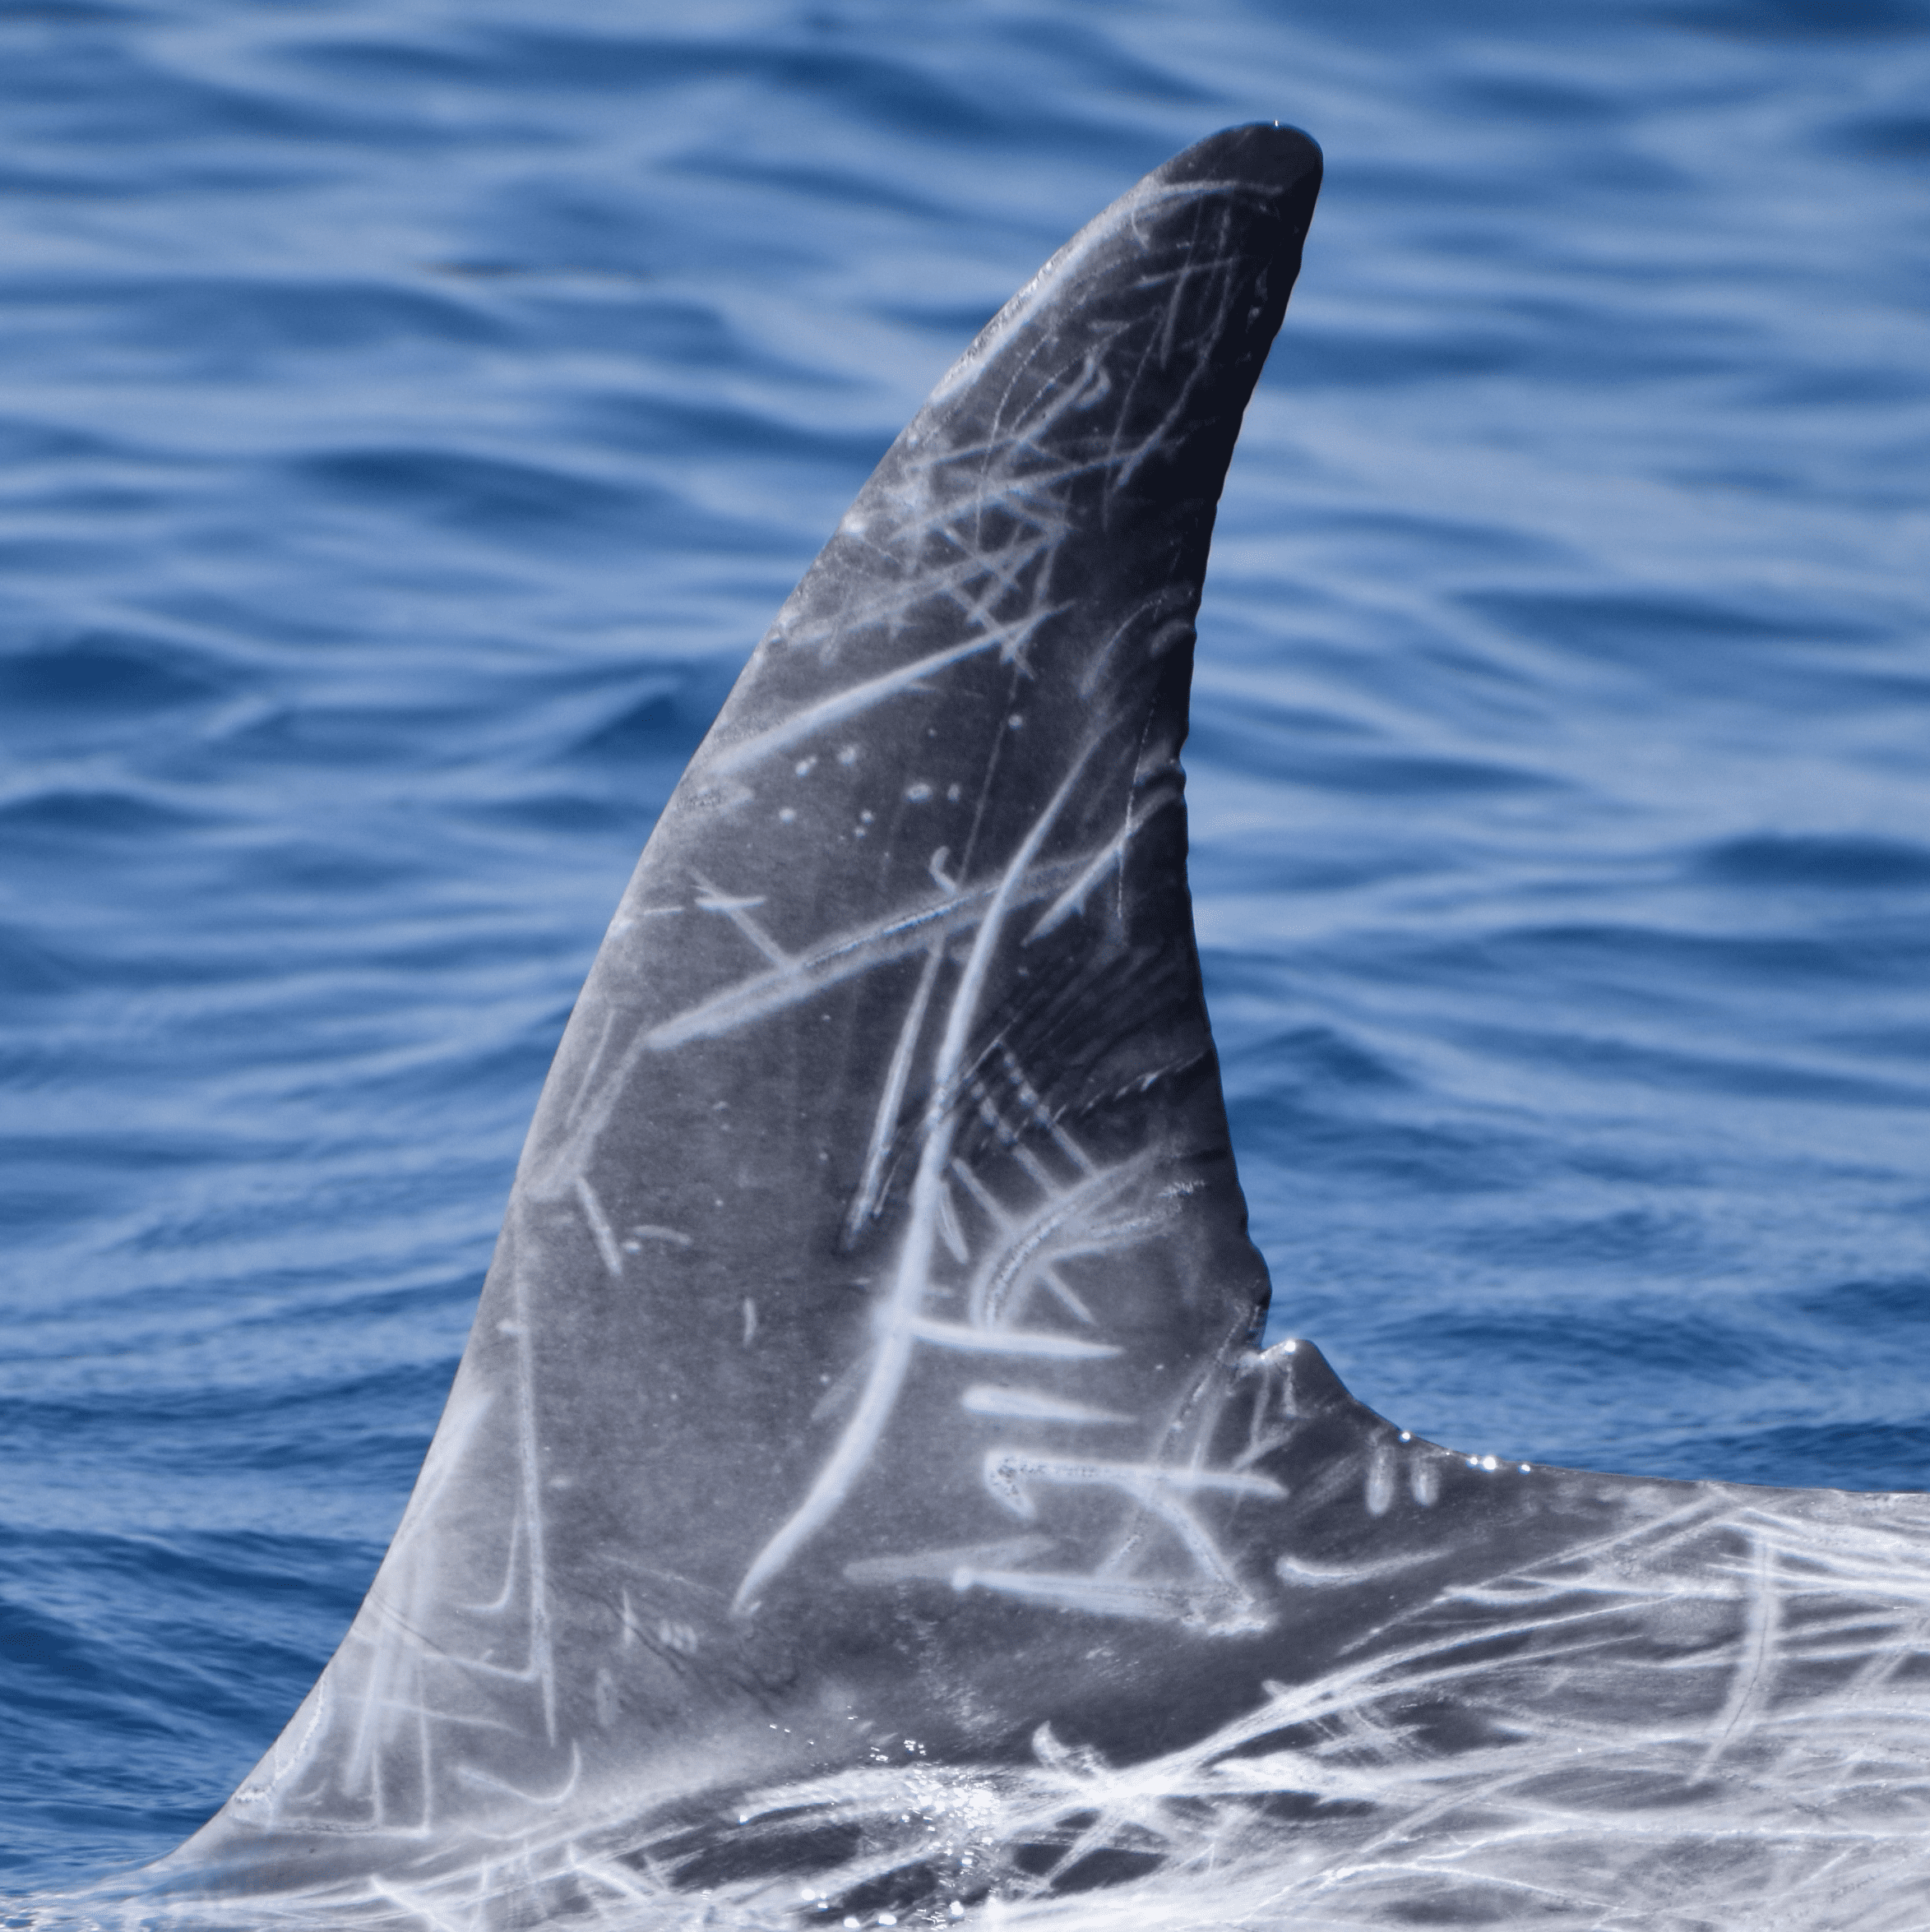
\includegraphics[width=\textwidth]{assets/images/methods/porting/features_extraction/original.png}   
        \caption{Immagine originale}
      \end{minipage}
      \begin{minipage}{0.3\textwidth}
        \centering
        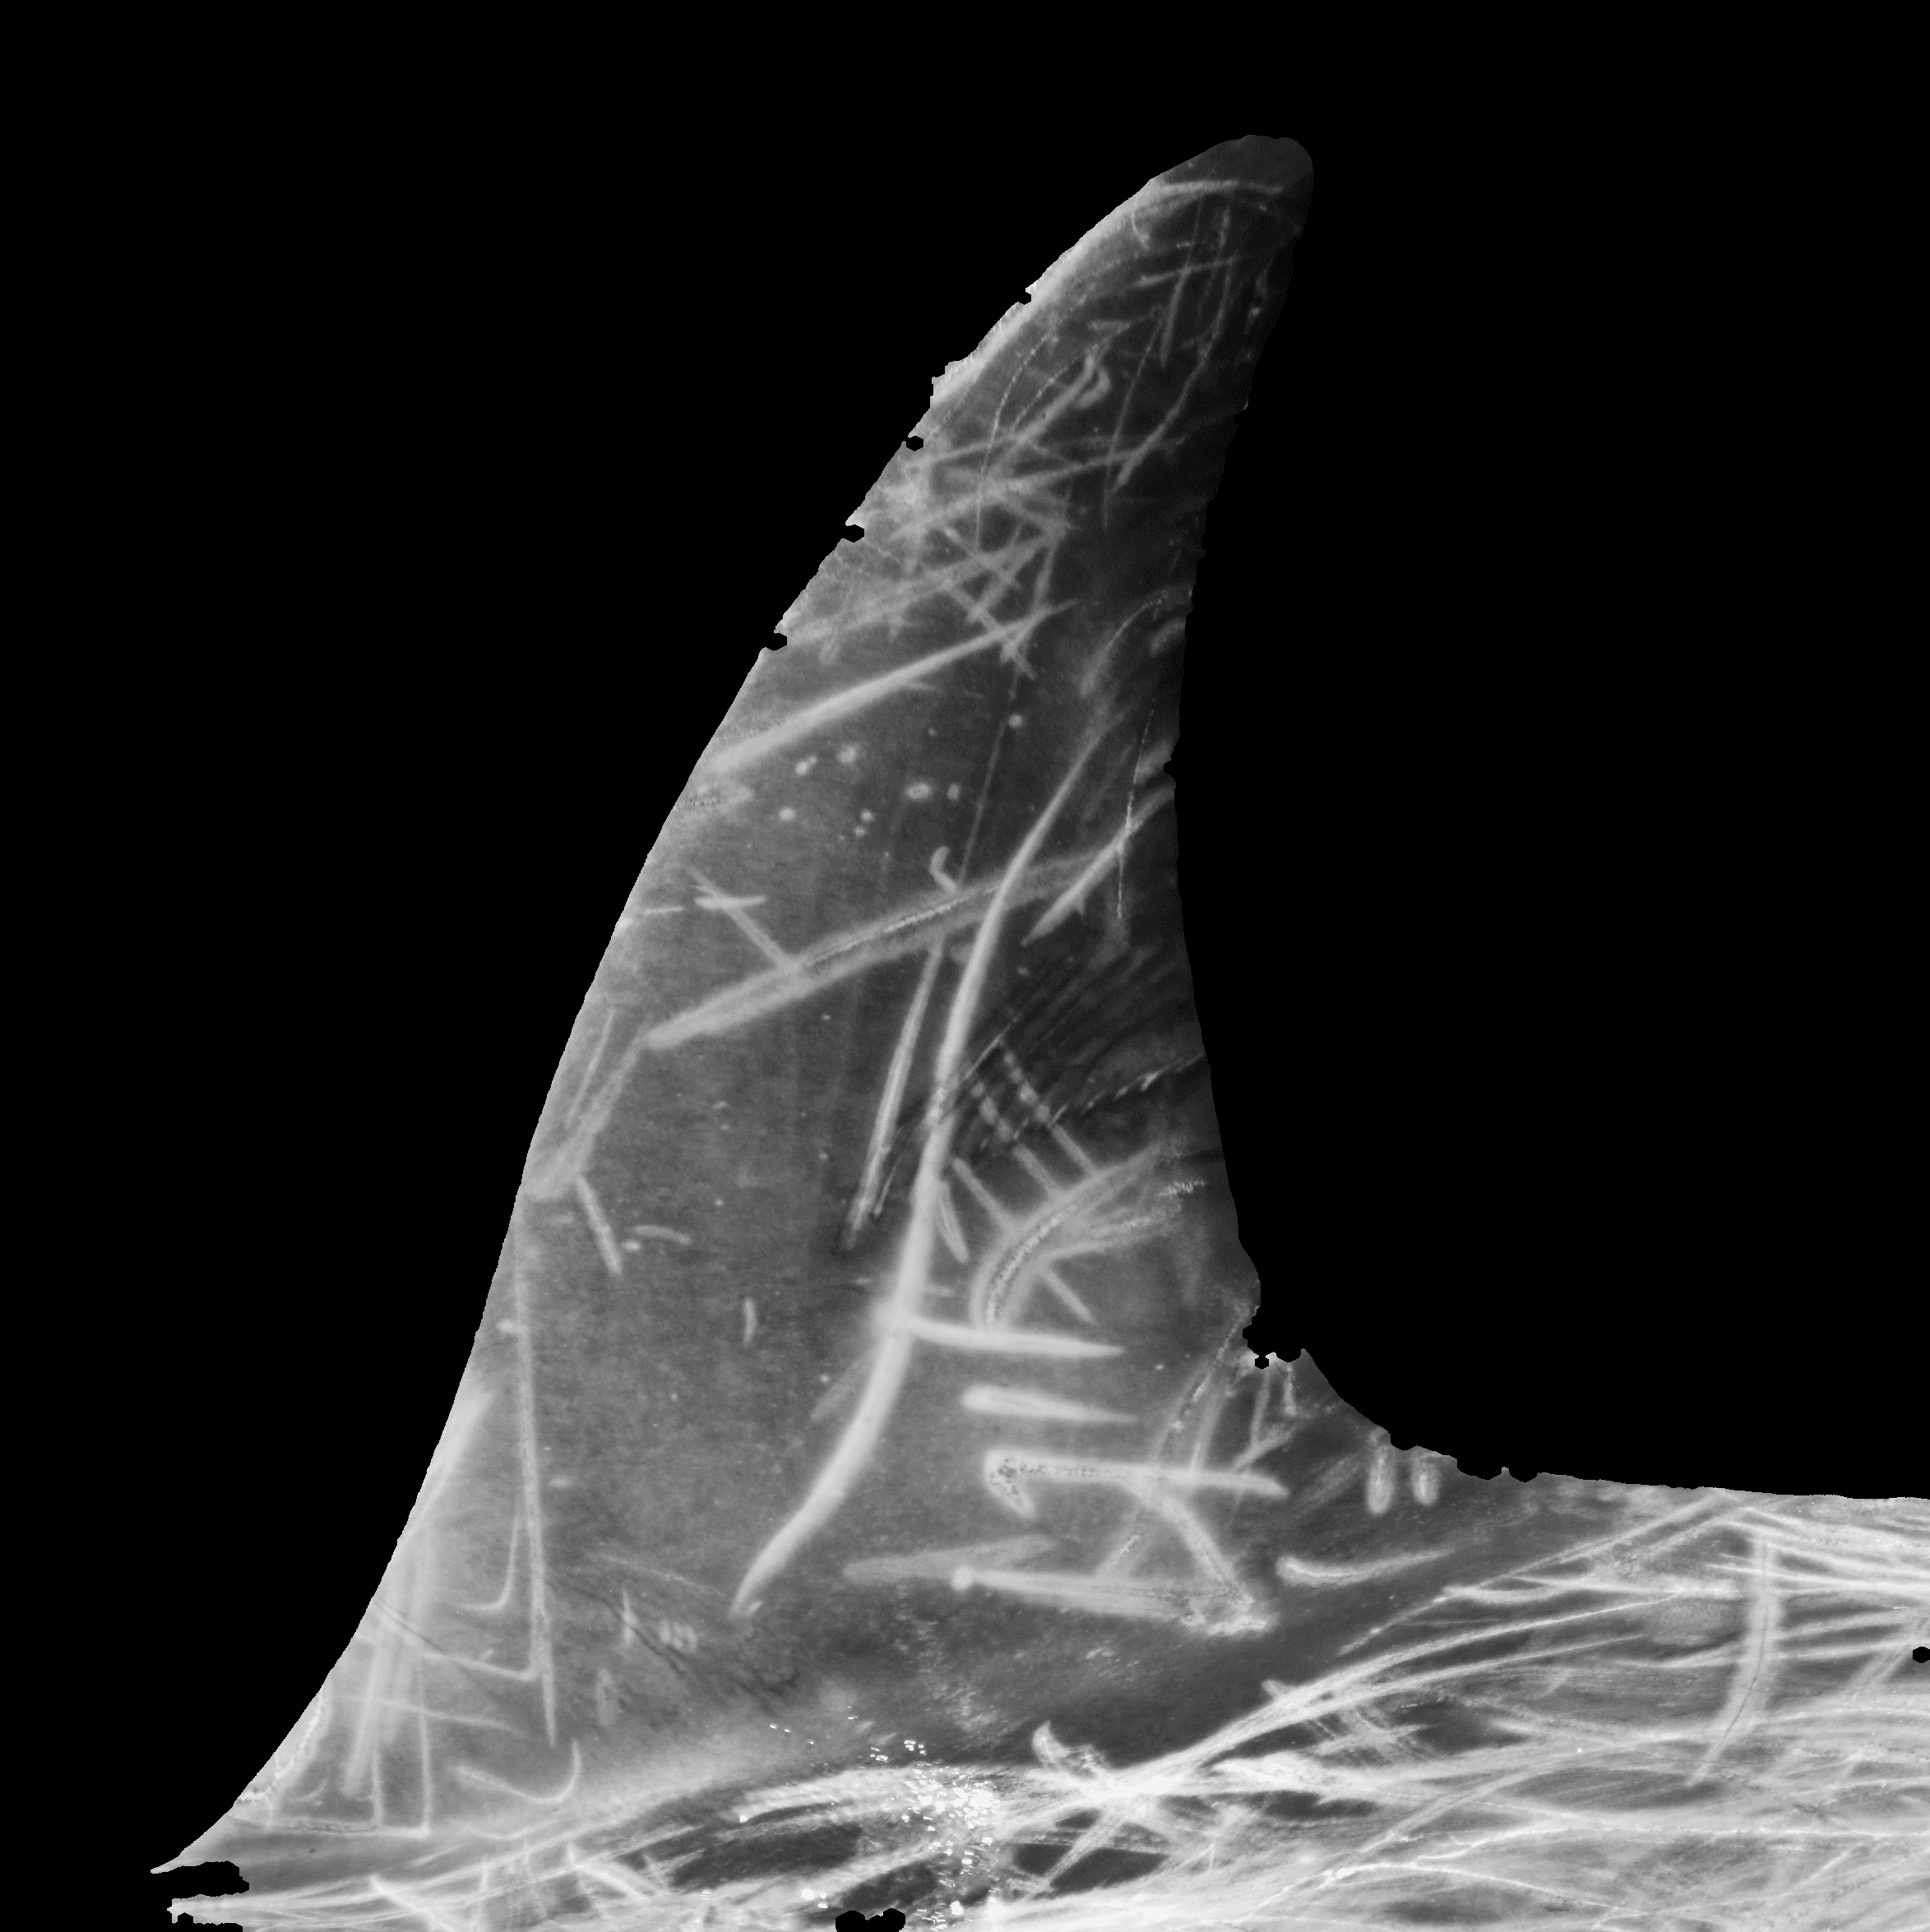
\includegraphics[width=\textwidth]{assets/images/methods/porting/features_extraction/gray.png}  
        \caption{Pinna estratta in scala di grigi}
      \end{minipage}
      \begin{minipage}{0.3\textwidth}
        \centering
        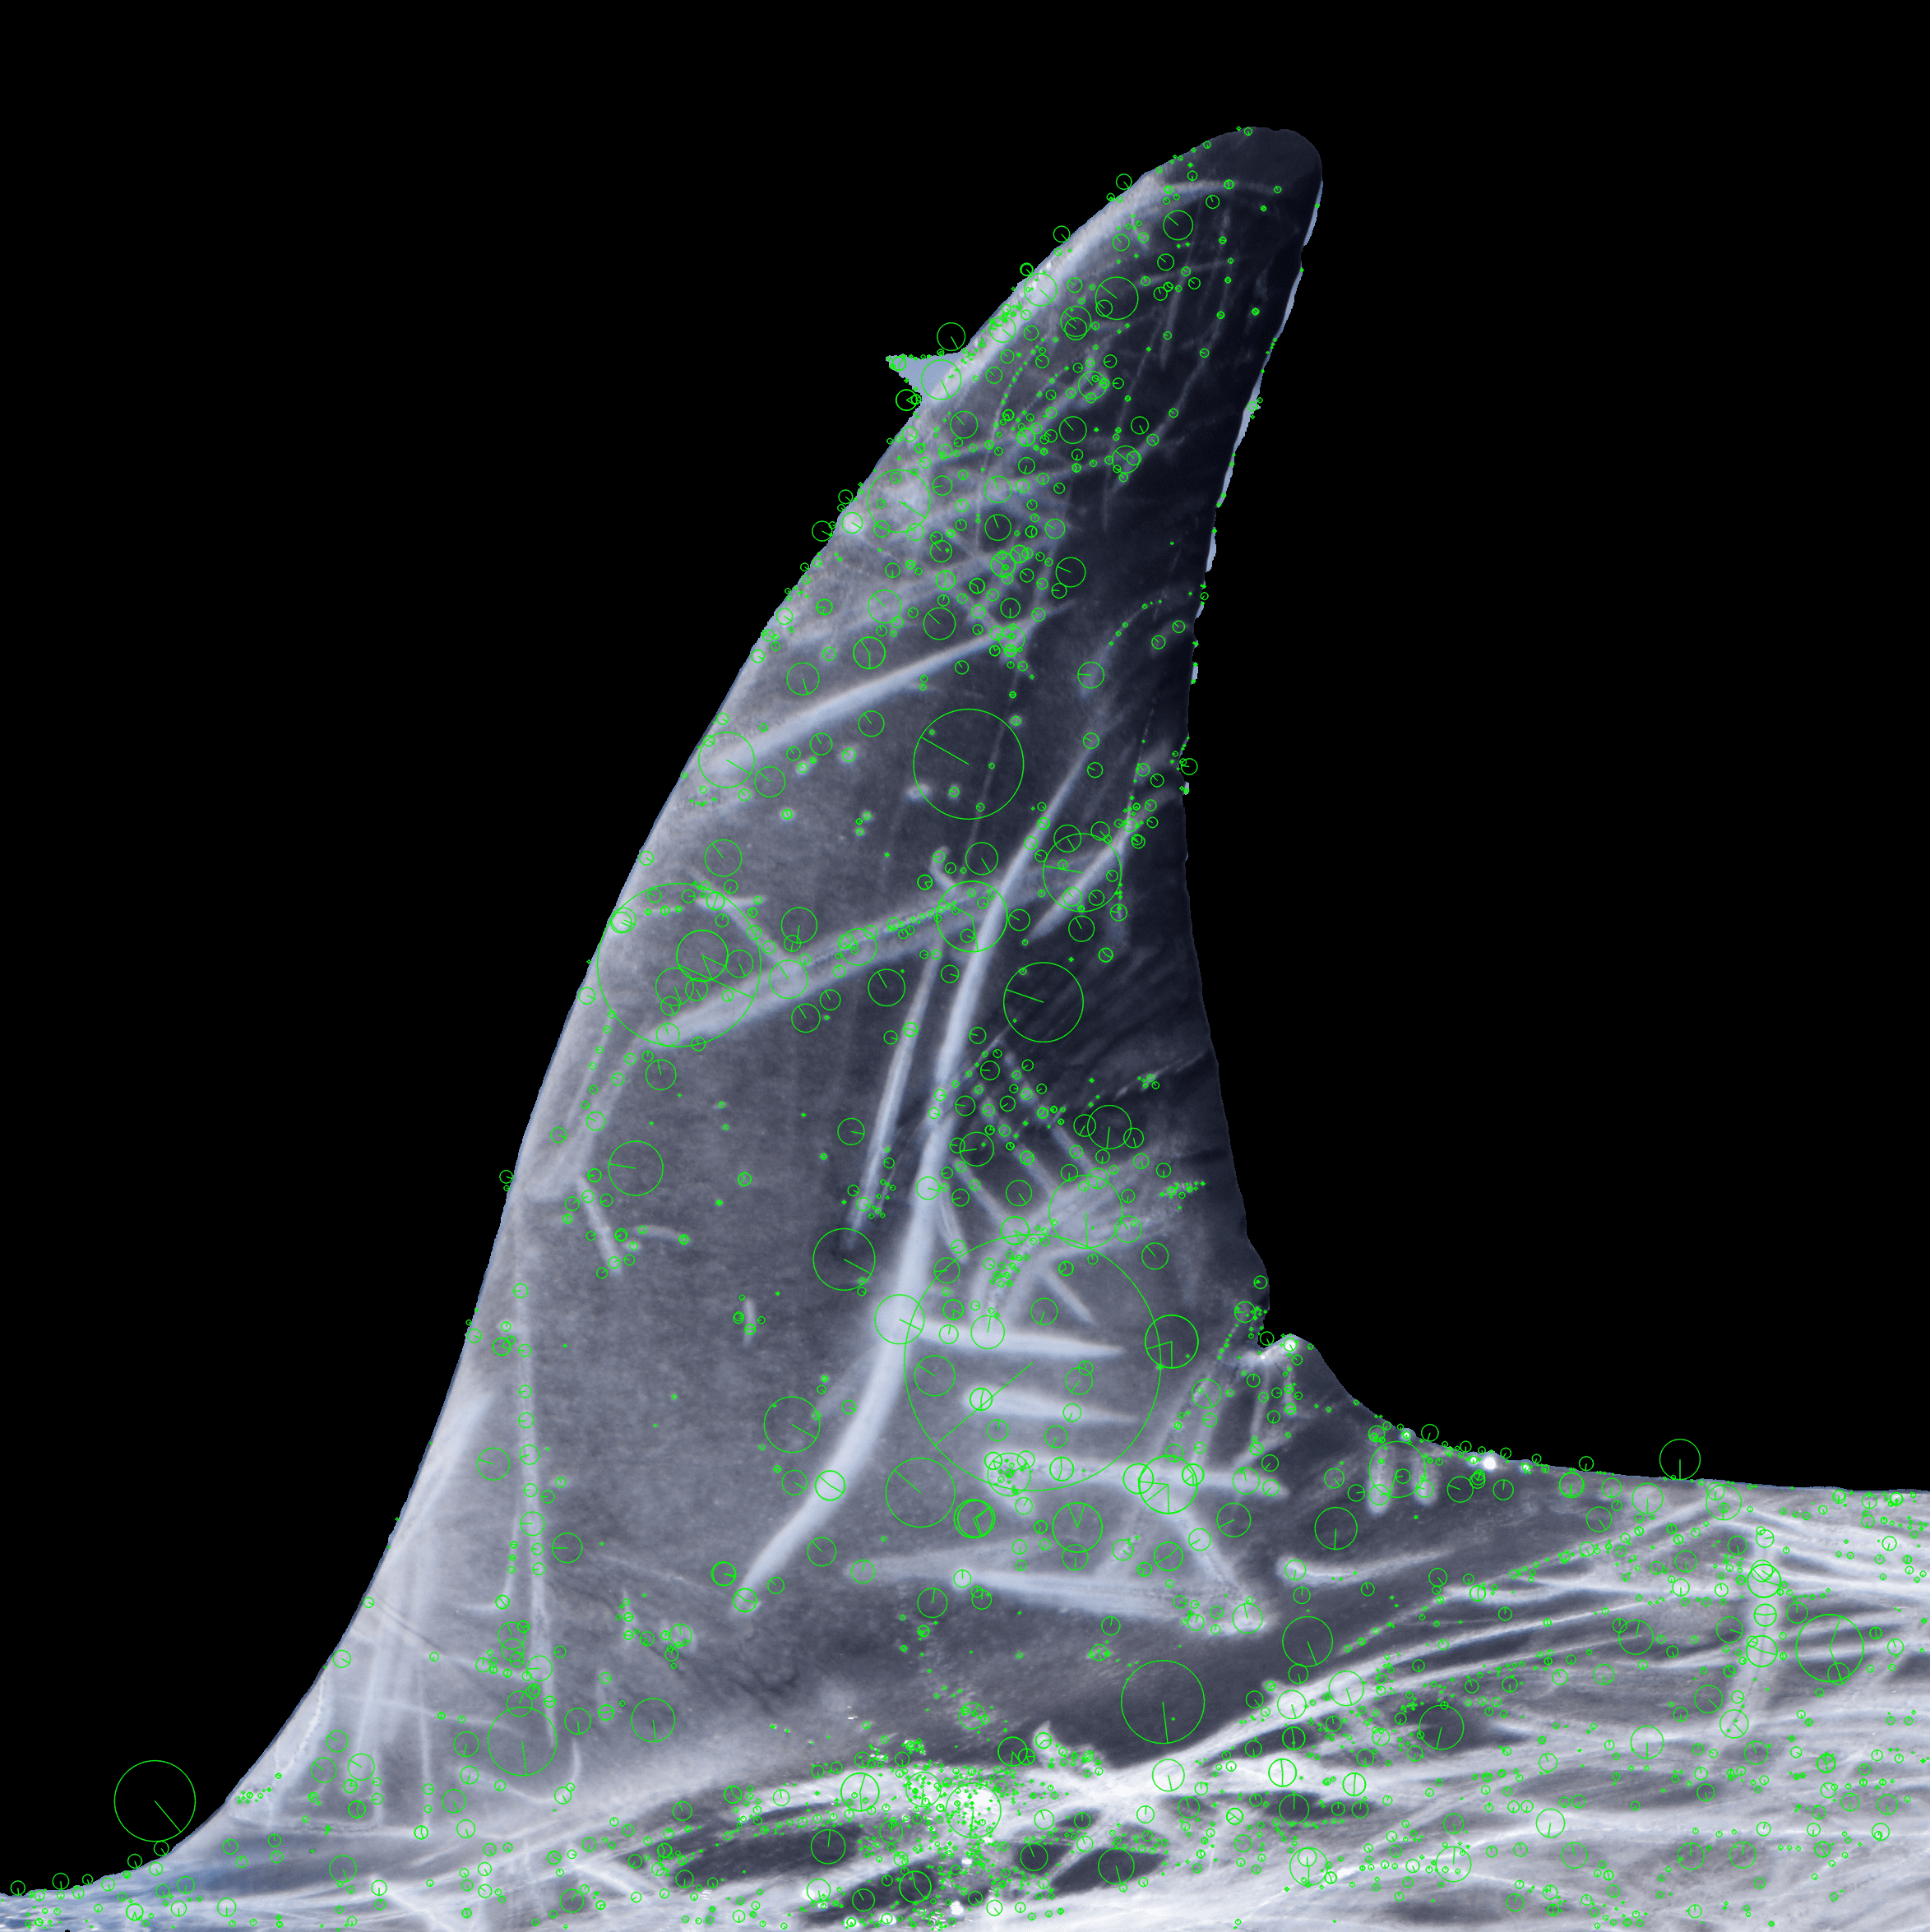
\includegraphics[width=\textwidth]{assets/images/methods/porting/features_extraction/features.png}   
        \caption{Features estratte}
      \end{minipage}
    \end{figure}

    A questo punto la maschera della pinna del delfino è stata estratta, 
    ora si può passare alla fase di feature extraction. Nello specifico l'algoritmo utilizzato 
    è Scale Invariant Feature Transform (SIFT), lo stesso della versione MATLAB,
    anche se nel corso dello sviluppo sono stati testati i seguenti algorimti di feature extraction:
    \begin{itemize}
      \item SIFT (Scale-Invariant Feature Transform \cite{lowe2004distinctive}): L'algoritmo SIFT è ampiamente utilizzato per estrarre features invarianti rispetto alla scala e alla rotazione. Rileva punti di interesse in un'immagine, calcola le loro descrizioni basate su gradienti di intensità e crea una rappresentazione compatta delle features. SIFT è noto per la sua robustezza rispetto alle variazioni di scala, rotazione, illuminazione e occlusioni.
      \item ORB (Oriented FAST and Rotated BRIEF \cite{rublee2011orb}): L'algoritmo ORB combina le caratteristiche di rilevazione rapida degli angoli (FAST) e il descrittore binario BRIEF. È un algoritmo efficiente che estrae features invarianti rispetto alla scala e all'orientazione. ORB utilizza un rilevatore di angoli per individuare punti di interesse, calcola gli orientamenti locali e genera descrittori binari per le feature.
      \newpage
      \item BRISK (Binary Robust Invariant Scalable Keypoints \cite{leutenegger2011brisk}): L'algoritmo BRISK è un metodo basato su descrittori binari che utilizza un rilevatore adattativo di punti di interesse. BRISK calcola un set di punti di interesse utilizzando un rilevatore adattativo basato su una rappresentazione piramidale dell'immagine. Successivamente, calcola i descrittori binari basati su informazioni di intensità e orientazione.
      \item AKAZE (Accelerated-KAZE \cite{alcantarilla2012fast}): L'algoritmo AKAZE è una variante accelerata dell'algoritmo KAZE, che a sua volta si basa sulla rilevazione di blob multiscale e sul calcolo di descrittori basati su regioni. AKAZE è noto per la sua robustezza alle variazioni di scala, rotazione, rumore e cambiamenti di illuminazione.
    \end{itemize}
\begin{lstlisting}
#La pinna estratta viene convertita in scala di grigi
gray_fin = cv2.cvtColor(fin, cv2.COLOR_BGR2GRAY)

#Vengono estratti keypoint e descrittori
#In modo analogo si estraggone le features con ORB, BRISK e AKAZE
sift = cv2.SIFT_create()
sift_keypoints, sift_descriptors = sift.detectAndCompute(gray_fin, None)

# Calcola la varianza dei descrittori
variances = np.var(sift_descriptors, axis=1)

# Soglia per la varianza per selezionare le features importanti
variance_threshold = 0.1

# Seleziona solo le features con varianza superiore alla soglia
selected_indices = np.where(variances > variance_threshold)[0]
sift_keypoints = [sift_keypoints[i] for i in selected_indices]
sift_descriptors = sift_descriptors[selected_indices]
\end{lstlisting}
      L'utilizzo della varianza come criterio per la selezione delle features si basa su una considerazione matematica fondamentale:
      la varianza misura la dispersione dei dati intorno alla loro media.
      In termini di feature extraction, la varianza può essere utilizzata 
      per valutare quanto le features variano all'interno di un set di dati.
      Features con varianza alta indicano una maggiore variabilità dei valori,
      mentre features con varianza bassa indicano una minore variabilità dei valori.
      L'idea di utilizzare la varianza per selezionare le features 
      più importanti si basa sul presupposto che le features più rilevanti 
      per un determinato compito o problema presentano una maggiore variabilità rispetto alle features meno rilevanti.
      Pertanto, selezionando le features con una varianza superiore a una soglia specificata, 
      si tende a mantenere le features che portano informazioni significative.
      \subsection{Salvataggio delle features}
      Il salvataggio delle features estratte è stato implementato tramite Protocol Buffer (protobuf
      ) \cite{protobuf} che è un meccanismo di serializzazione dei dati sviluppato da Google.
      È un formato di scambio di dati binario che consente di definire la struttura 
      dei dati in modo dichiarativo utilizzando un file di definizione del protocollo (.proto).
      Questo file di definizione specifica i tipi di dati e i messaggi che possono essere trasmessi utilizzando Protobuf.

      Protobuf offre diverse caratteristiche e vantaggi rispetto ad altri formati di serializzazione dei dati come XML e JSON.
      Alcune delle caratteristiche principali di Protobuf includono:
      \begin{itemize}
        \item Efficienza: I dati serializzati con Protobuf sono più compatti rispetto ad altri formati come JSON o XML, risultando in dimensioni di dati più ridotte. Questo porta a un minor utilizzo dello spazio di archiviazione e una trasmissione più veloce dei dati su una rete.
        \newpage
        \item Velocità: La serializzazione e deserializzazione dei dati utilizzando Protobuf sono molto efficienti e veloci. I dati possono essere facilmente convertiti in un formato binario e viceversa, garantendo prestazioni elevate.
        \item Interoperabilità: I file di definizione del protocollo (.proto) consentono di generare codice sorgente in diverse lingue di programmazione, inclusi C++, Java, Python, Dart e molti altri. Questo facilita l'interoperabilità tra diversi sistemi che utilizzano linguaggi di programmazione diversi.
        \item Tipizzazione forte: Protobuf definisce tipi di dati specifici nel file di definizione del protocollo, consentendo una tipizzazione forte durante la serializzazione e deserializzazione dei dati. Ciò offre un maggiore controllo sui dati trasmessi e contribuisce a ridurre gli errori di interpretazione dei dati.
      \end{itemize}
      \newpage
      \subsection{Match feature}
      \begin{figure}[H]
        \centering
        \centering
        \includegraphics[width=\textwidth]{assets/images/methods/porting/features_match/match.png}   
        \caption{Match delle feature}
      \end{figure}


      Dopo il salvataggio del dataset contenente tutti i keypoint e descrittori 
      \\ per ogni immagine, raggruppati per nome del delfino (modello), si è passato ad implementare il match con OpenCV. \\
      In OpenCV, ci sono diverse strategie di match di features che possono essere utilizzate per confrontare e cercare corrispondenze tra le caratteristiche estratte da diverse immagini. Di seguito sono elencate alcune delle strategie più comuni:

      \begin{itemize}
        \item Brute-Force Matching: Questa è la strategia più semplice, in cui ogni caratteristica estratta dall'immagine di query viene confrontata con tutte le caratteristiche estratte dall'immagine di train. Questo metodo può essere computazionalmente costoso se il numero di caratteristiche è elevato.
        \newpage
        \item K-Nearest Neighbors (KNN) Matching \cite{knn}: Invece di confrontare ogni caratteristica dell'immagine di query con tutte le caratteristiche dell'immagine di train, questo approccio seleziona i K punti più vicini (più simili) per ogni caratteristica estratta dall'immagine di query. Può essere usato il modulo FlannBasedMatcher per utilizzare un algoritmo di ricerca dell'albero kd-tree per migliorare l'efficienza.
        \item RANSAC (Random Sample Consensus) \cite{ransac}: È una tecnica robusta per stimare i parametri di un modello matematico da un set di dati che contiene outlier. Nell'ambito del match di features, RANSAC può essere utilizzato per stimare la trasformazione geometrica (ad esempio, una trasformazione affina o una trasformazione prospettica) tra due immagini.
        \item Lowe's Ratio Test \cite{lowe2004distinctive}: Questo test viene utilizzato per filtrare le corrispondenze deboli. Per ogni caratteristica estratta, si confronta il rapporto tra la distanza euclidea della migliore corrispondenza e la distanza euclidea della seconda migliore corrispondenza. Se il rapporto è inferiore a una soglia predefinita, la corrispondenza viene accettata.
      \end{itemize}

\newpage
      \begin{lstlisting}

#...
# Cicla su tutti i modelli del dataset
for model in dataset.models:
    # Cicla su tutte le s del modello
    for model_data2 in model.data:
        k2 = convert_keypoints(model_data2.keypoints)
        d2 = convert_descriptors(model_data2.descriptors)

        # Crea un oggetto BFMatcher (Brute-Force Matcher)
        bf = cv2.BFMatcher()

        # Trova i migliori abbinamenti tra i descrittori dell'immagine di query e del dataset
        matches = bf.knnMatch(d1, d2, k=2)

        # Verifica se ci sono abbastanza abbinamenti
        if len(matches) < 2:
            continue
        # Calcola la distanza media dei migliori abbinamenti
        total_distance = 0
        for m, n in matches:
            total_distance += m.distance
        
        average_distance = total_distance / len(matches)

        # Se la distanza media è migliore del miglior match attuale, aggiorna i valori
        if average_distance < 280 and average_distance < best_match_distance:
            best_match = model_data.file_name
            best_match_distance = average_distance

            data[model.name] = average_distance
#...
      \end{lstlisting}
      La strategia KNN (K-Nearest Neighbors) è stata scelta per effettuare il match delle features estratte dalle pinne di delfino per diversi motivi. Il KNN è un algoritmo di apprendimento supervisionato utilizzato per la classificazione e il riconoscimento dei pattern. 
      \newpage
      È un metodo semplice ma efficace per la classificazione basata sulla vicinanza dei punti nel suo spazio delle features.
      Nel contesto del riconoscimento delle pinne di delfino, le features estratte, come ad esempio i descrittori SIFT (Scale-Invariant Feature Transform), rappresentano le caratteristiche distintive delle pinne. Queste features possono includere informazioni come orientamento, forma e disposizione dei punti chiave delle pinne.
      L'obiettivo principale di utilizzare l'algoritmo KNN in questo caso è quello di trovare le corrispondenze più simili tra le features estratte dalle diverse pinne. Il funzionamento del KNN prevede che, dato un punto di input (cioè una features estratta da una pinna), l'algoritmo confronti questo punto con i punti di allenamento (features estratte da altre pinne) e determini i "K" punti di allenamento più vicini in base a una misura di distanza. In seguito, il punto di input viene classificato in base alla maggioranza dei K punti di allenamento più vicini.
      Nel caso delle pinne di delfino, l'algoritmo KNN può essere utilizzato per confrontare le features estratte da una pinna non identificata con un insieme di features di pinne di delfino precedentemente raccolte e classificate (dataset). In altre parole, le features estratte dalle pinne di delfino sconosciute possono essere confrontate con le features delle pinne di delfino note, e l'algoritmo KNN può essere utilizzato per determinare a quale pinna conosciuta la pinna sconosciuta è più simile.
      La scelta del valore "K" nel KNN è importante e dipende dal contesto specifico. Un valore "K" più piccolo può portare a una classificazione più sensibile al rumore o alle variazioni casuali, mentre un valore "K" più grande può portare a una classificazione più robusta ma potenzialmente meno sensibile alle differenze sottili tra le pinne.
      In sintesi, la strategia KNN è stata scelta per il match delle features estratte dalle pinne di delfino perché permette di confrontare le caratteristiche distintive delle pinne sconosciute con quelle delle pinne conosciute, consentendo di identificare la corrispondenza più simile.





      \newpage
    \section{Estrazione maschera con Deep Learning}
      Durante lo svilupppo del porting, è nata l'esigenza di creare un dataset
      composto da vere maschere create a mano, per avere un metro di paragone da
      utilizzare con la precedente versione di SPIR per stabilire i progressi fatti nell'estrazione
      delle maschere, proprio questa necessità ha fornito l'idea per lo studio paralello di
      una rete neurale di tipo deep learning, avente l'obiettivo di estrarre le maschere per il 
      ritaglio delle pinne di delfino.
      L'intero sviluppo della rete neurale è stato fatto 
      nell'ambiente virtuale di Google Colab \cite{colab}, grazie ad esso è stato 
      possibile sfruttare GPU e TPU per l'addestramento del modello, andando a velocizzare i tempi.
      \subsection{Dataset}
      \begin{figure}[H]
        \centering
        \begin{minipage}{0.4\textwidth}
          \centering
          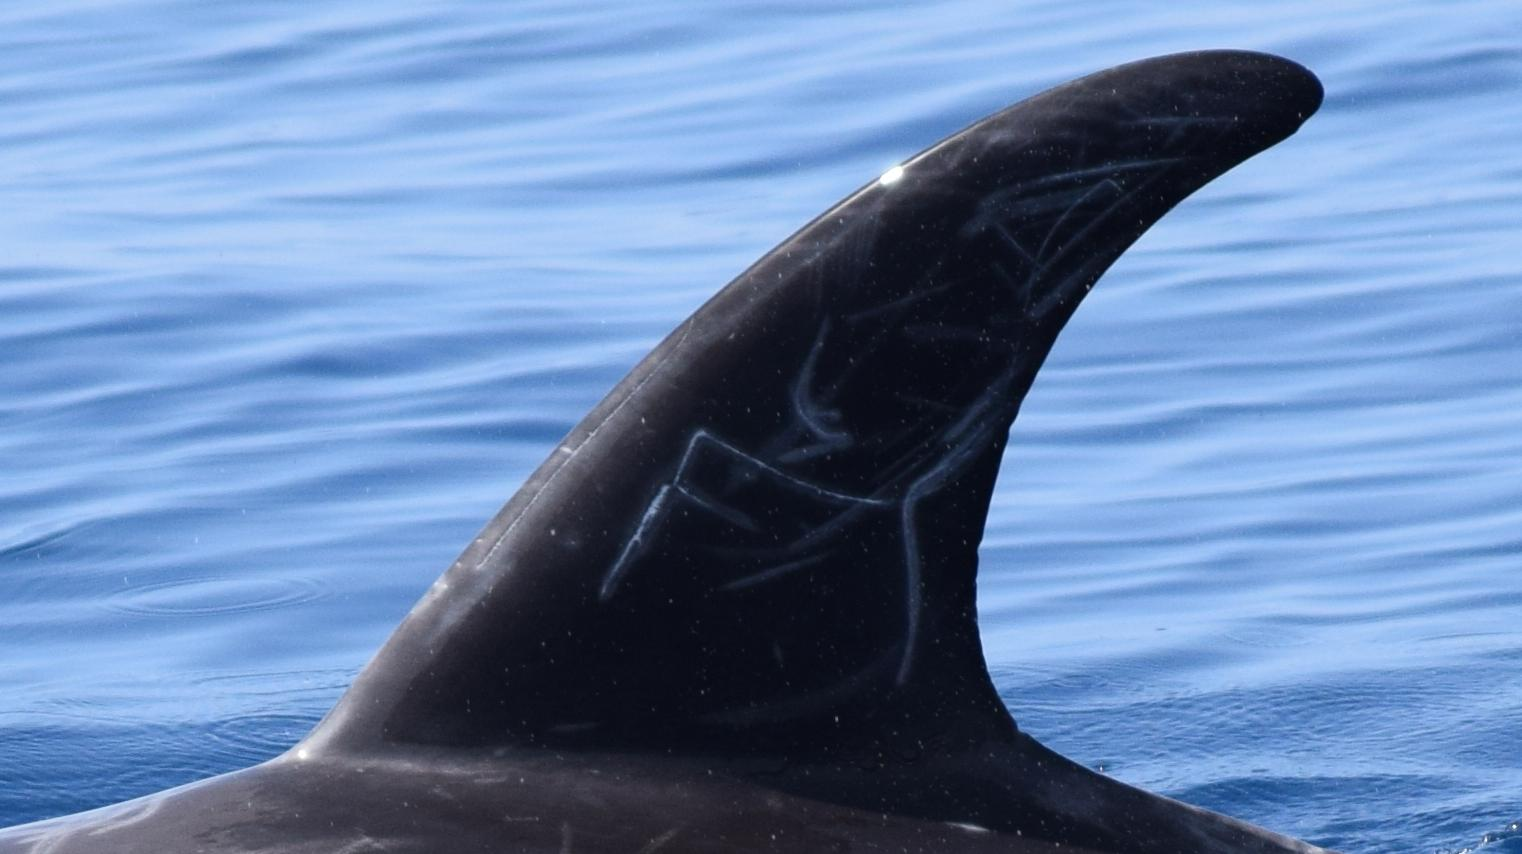
\includegraphics[width=\textwidth]{assets/images/methods/deep/dataset/original.png}   
          \caption{Immagine originale}
        \end{minipage}
        \begin{minipage}{0.4\textwidth}
          \centering
          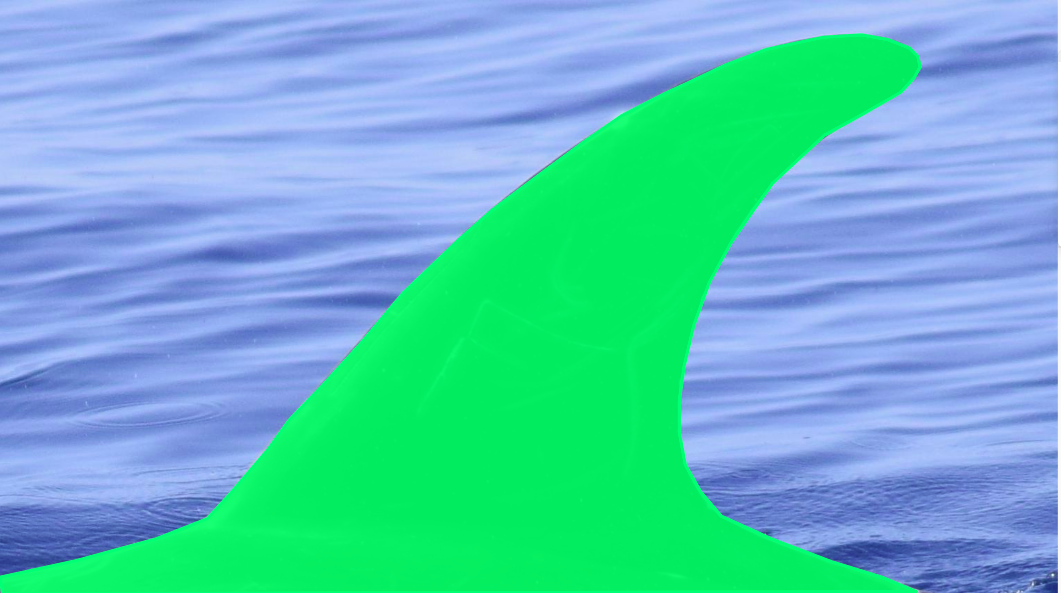
\includegraphics[width=\textwidth]{assets/images/methods/deep/dataset/mask.png}   
          \caption{Maschera poligono}
        \end{minipage}
      \end{figure}
      Il dataset è stato creato utilizzando il software open source Label Studio \cite{labelstudio}, il quale è stato installato su un server
      remoto, ciò ha permesso di accedere facilmente da browser, il software offre due tipi di 
      template per Object Segmentation:
      \begin{itemize}
        \item Maschere: le annotazioni sono rappresentate come maschere binarie che indicano l'area esatta degli oggetti di interesse. Ogni pixel può essere 1 (oggetto) o 0 (sfondo).
        \item Poligoni: le annotazioni sono rappresentate come contorni poligonali che delimitano l'area degli oggetti. Sono definite da una serie di vertici o punti che seguono i contorni degli oggetti.
      \end{itemize}
      In questo caso è stato scelto di utilizzare un dataset basato su label di tipo poligonale,
      questo dettato anche dalla velocità di creazione dei poligoni, un minor costo computazionale 
      di calcolo rispetto a dataset basato su maschere.
      In totale si è lavorato su un dataset di 1725 foto, delle quali per ragioni
      di tempo "solo" 150 sono state descritte con maschere poligonali. 
      Come formato di salvataggio del dataset è stato scelto COCO \cite{coco}, 
      per i seguenti motivi:
      \begin{itemize}
        \item Struttura organizzata: Il formato COCO offre una struttura ben definita per il dataset di segmentazione degli oggetti. Fornisce una gerarchia chiara per le annotazioni, le immagini e le categorie degli oggetti, semplificando l'organizzazione e la gestione dei dati.
        \item Annotazioni precise: COCO consente di annotare gli oggetti di interesse all'interno delle immagini utilizzando maschere o poligoni, permettendo una rappresentazione accurata delle aree degli oggetti. Questo consente di addestrare modelli di segmentazione più precisi e dettagliati.
        \item Metriche di valutazione standard: COCO fornisce metriche di valutazione standard per valutare le prestazioni dei modelli di segmentazione degli oggetti. Questo facilita il confronto tra i diversi approcci e la valutazione delle prestazioni in modo coerente e affidabile.
        \item Ampia comunità e risorse: Il formato COCO è supportato da una vasta comunità di ricercatori e sviluppatori nel campo della visione artificiale. Ciò significa che ci sono molte risorse, strumenti e modelli disponibili per lavorare con il formato COCO, semplificando lo sviluppo e la sperimentazione di nuovi metodi di segmentazione degli oggetti.
      \end{itemize}
      \newpage
      \subsection{Struttura Rete}
      Tra le varie alternative disponibili nel panorama delle librerie Python per ML e Deep,
      la scelta è stata guidata dal miglior compromesso in termini di flessibilità e scalabilità,
      anche in vista di sviluppi futuri del codice, questo ha portato a scegliere
      TensorFlow \cite{tensorflow} come libreria, evidenziando i seguenti vantaggi:
      \begin{itemize}
        \item Ampia adozione e supporto della comunità: TensorFlow è uno dei framework di deep learning più popolari ed è ampiamente utilizzato in ambito accademico e industriale. Ciò significa che ci sono molte risorse, documentazione, tutorial e una vasta comunità di sviluppatori pronti a fornire supporto.
        \item Ecosistema completo: TensorFlow fornisce un ecosistema completo per la creazione e la distribuzione di modelli di machine learning. Include strumenti per la pre-elaborazione dei dati, la creazione dei modelli, l'addestramento, l'ottimizzazione e l'inferenza.
        \item Scalabilità e prestazioni: TensorFlow è stato progettato per sfruttare appieno le risorse hardware disponibili, inclusi processori multi-core, GPU e TPU. Questo consente di ottenere prestazioni elevate e di sfruttare al meglio le risorse hardware disponibili.
        \item Supporto multi-piattaforma: TensorFlow è supportato su diverse piattaforme, tra cui desktop, server, dispositivi mobili e dispositivi IoT. Ciò consente di creare modelli una volta e distribuirli su diverse piattaforme senza dover ripensare completamente l'implementazione.
      \end{itemize}
      \newpage
      Avendo il dataset pronto in formato COCO, non è stato difficile passare al
      caricamento e creazione del dataset in TensorFlow, 
      dato che il formato COCO salva i modelli e i relativi label
      in formato JSON è stato necessario creare un metodo per il 
      parsing, da JSON a TFRecord, questo permette di lavorare su 
      un tipo di dataset composto da righe, con anche la possibilità
      di salvare il dataset in diversi file .tfrecord di dimensioni fissate
      così da ottimizzare le operazioni di caricamento del dataset in memoria. 
      \begin{lstlisting}
class Augment(tf.keras.layers.Layer):
  #Viene impostato il seed per avere sempre la stessa generazione
  def __init__(self, seed=42):
    super().__init__()
    self.augment_inputs = tf.keras.layers.RandomFlip(mode="horizontal", seed=seed)
    
    self.augment_inputs_rotation = tf.keras.layers.RandomRotation(factor=0.2, seed=seed)
    
    self.augment_inputs_zoom = tf.keras.layers.RandomZoom(height_factor=(-0.2, 0.2), width_factor=(-0.2, 0.2), seed=seed)
#...
      \end{lstlisting}
      Data la scarsa quantità di modelli descritti da poligoni nel dataset (solo 150)
      si è optato per applicare tecniche di data augmentation o aumento di dati tra cui: riflessione, ingrandimento e rotazione,
      queste trasformazioni vengono applicate naturalmente sia al modello (foto del delfino) 
      e sia al poligono che ne descrive la maschera 
      della pinna, la scelta se applicare una delle trasformazioni al modello è fatta in modo 
      casuale dai metodi di TensorFlow (tf.keras.layers).
    
      \begin{figure}[H]
        \centering
        \begin{minipage}{0.8\textwidth}
          \centering
          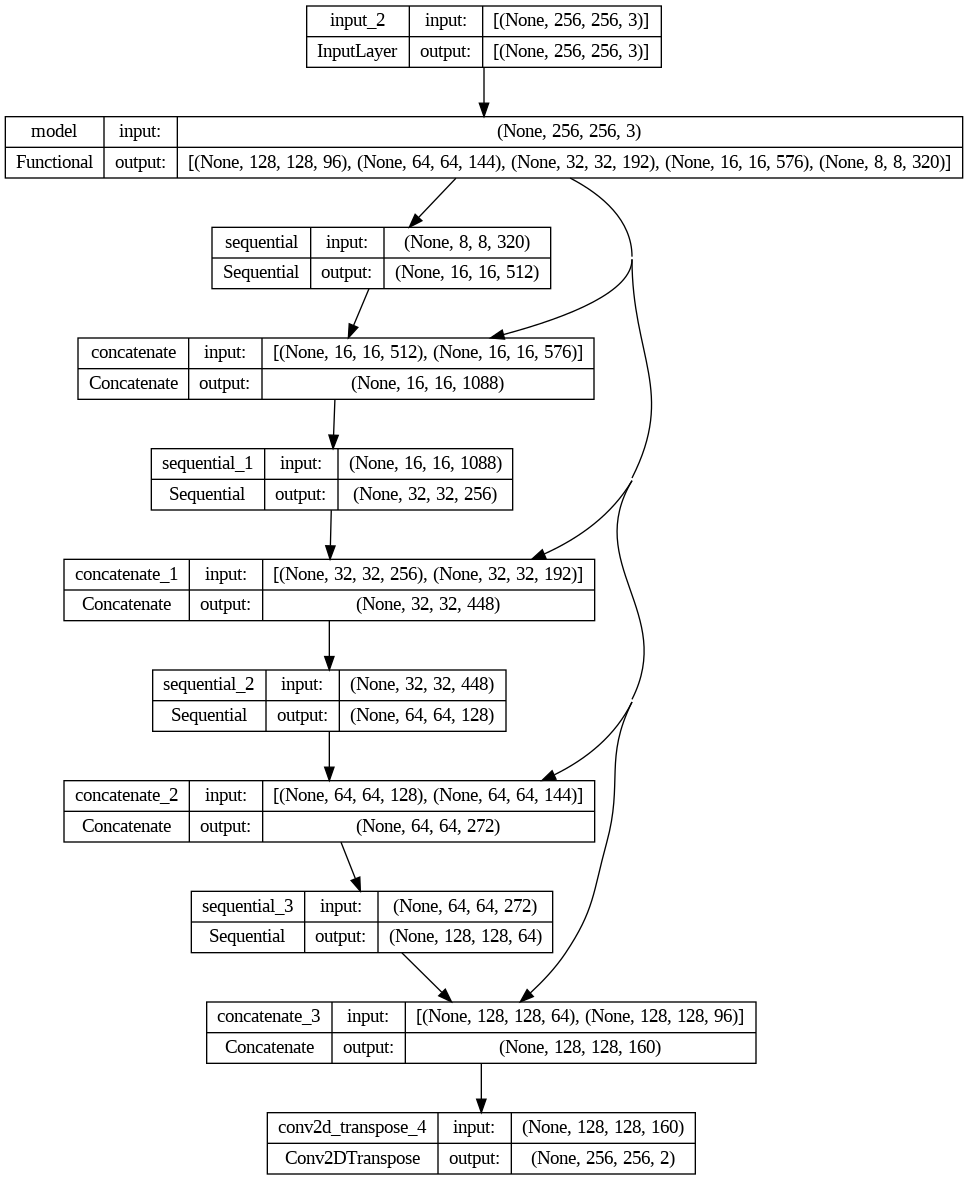
\includegraphics[width=\textwidth]{assets/images/methods/deep/network/network.png}   
          \caption{Struttura rete neurale}
        \end{minipage}
      \end{figure}
      Una volta costruito il dataset in formato TFRecordDataset si può passare
      alla struttura della rete, come modello per effettuare Object Segmentation
      è stato scelto U-Net \cite{ronneberger2015u},
      \\ 
      U-Net è un modello di rete neurale che si è dimostrato efficace per la segmentazione delle immagini,
      compresa la creazione di maschere per oggetti di forma complessa come le pinne di delfino.
      \newpage
      Le caratteristiche chiave di U-Net che lo rendono un buon modello per questo compito sono:

      \begin{itemize}
        \item Architettura a forma di U: U-Net utilizza un'architettura a forma di U, che combina un percorso di contrazione (encoder) con un percorso di espansione (decoder). Questa struttura consente di catturare dettagli a diverse scale e di ricostruire con precisione le forme complesse delle pinne di delfino.
        \item Connessioni skip: U-Net incorpora connessioni skip tra le diverse profondità dell'encoder e del decoder. Queste connessioni consentono di preservare le informazioni a diverse scale spaziali durante il processo di up-sampling, aiutando a ripristinare dettagli fini nelle maschere delle pinne di delfino.
        \item Utilizzo di convoluzioni e pooling: U-Net utilizza convoluzioni e operazioni di pooling per estrarre progressivamente le caratteristiche delle immagini in diverse profondità. Questo aiuta il modello a identificare gli elementi distintivi delle pinne di delfino e a discriminare tra le regioni di interesse e lo sfondo.
        \item Utilizzo di dati di addestramento limitati: U-Net è stato progettato per funzionare bene anche con dataset di addestramento limitati. La sua architettura compatta e le connessioni skip consentono di ottenere buone prestazioni anche con un numero ridotto di esempi di addestramento.
      \end{itemize}
    %\subsection{Training}
    %\subsection{Generazione maschera}

    \section{Sistema SPIR}
    \begin{figure}[H]
      \centering
      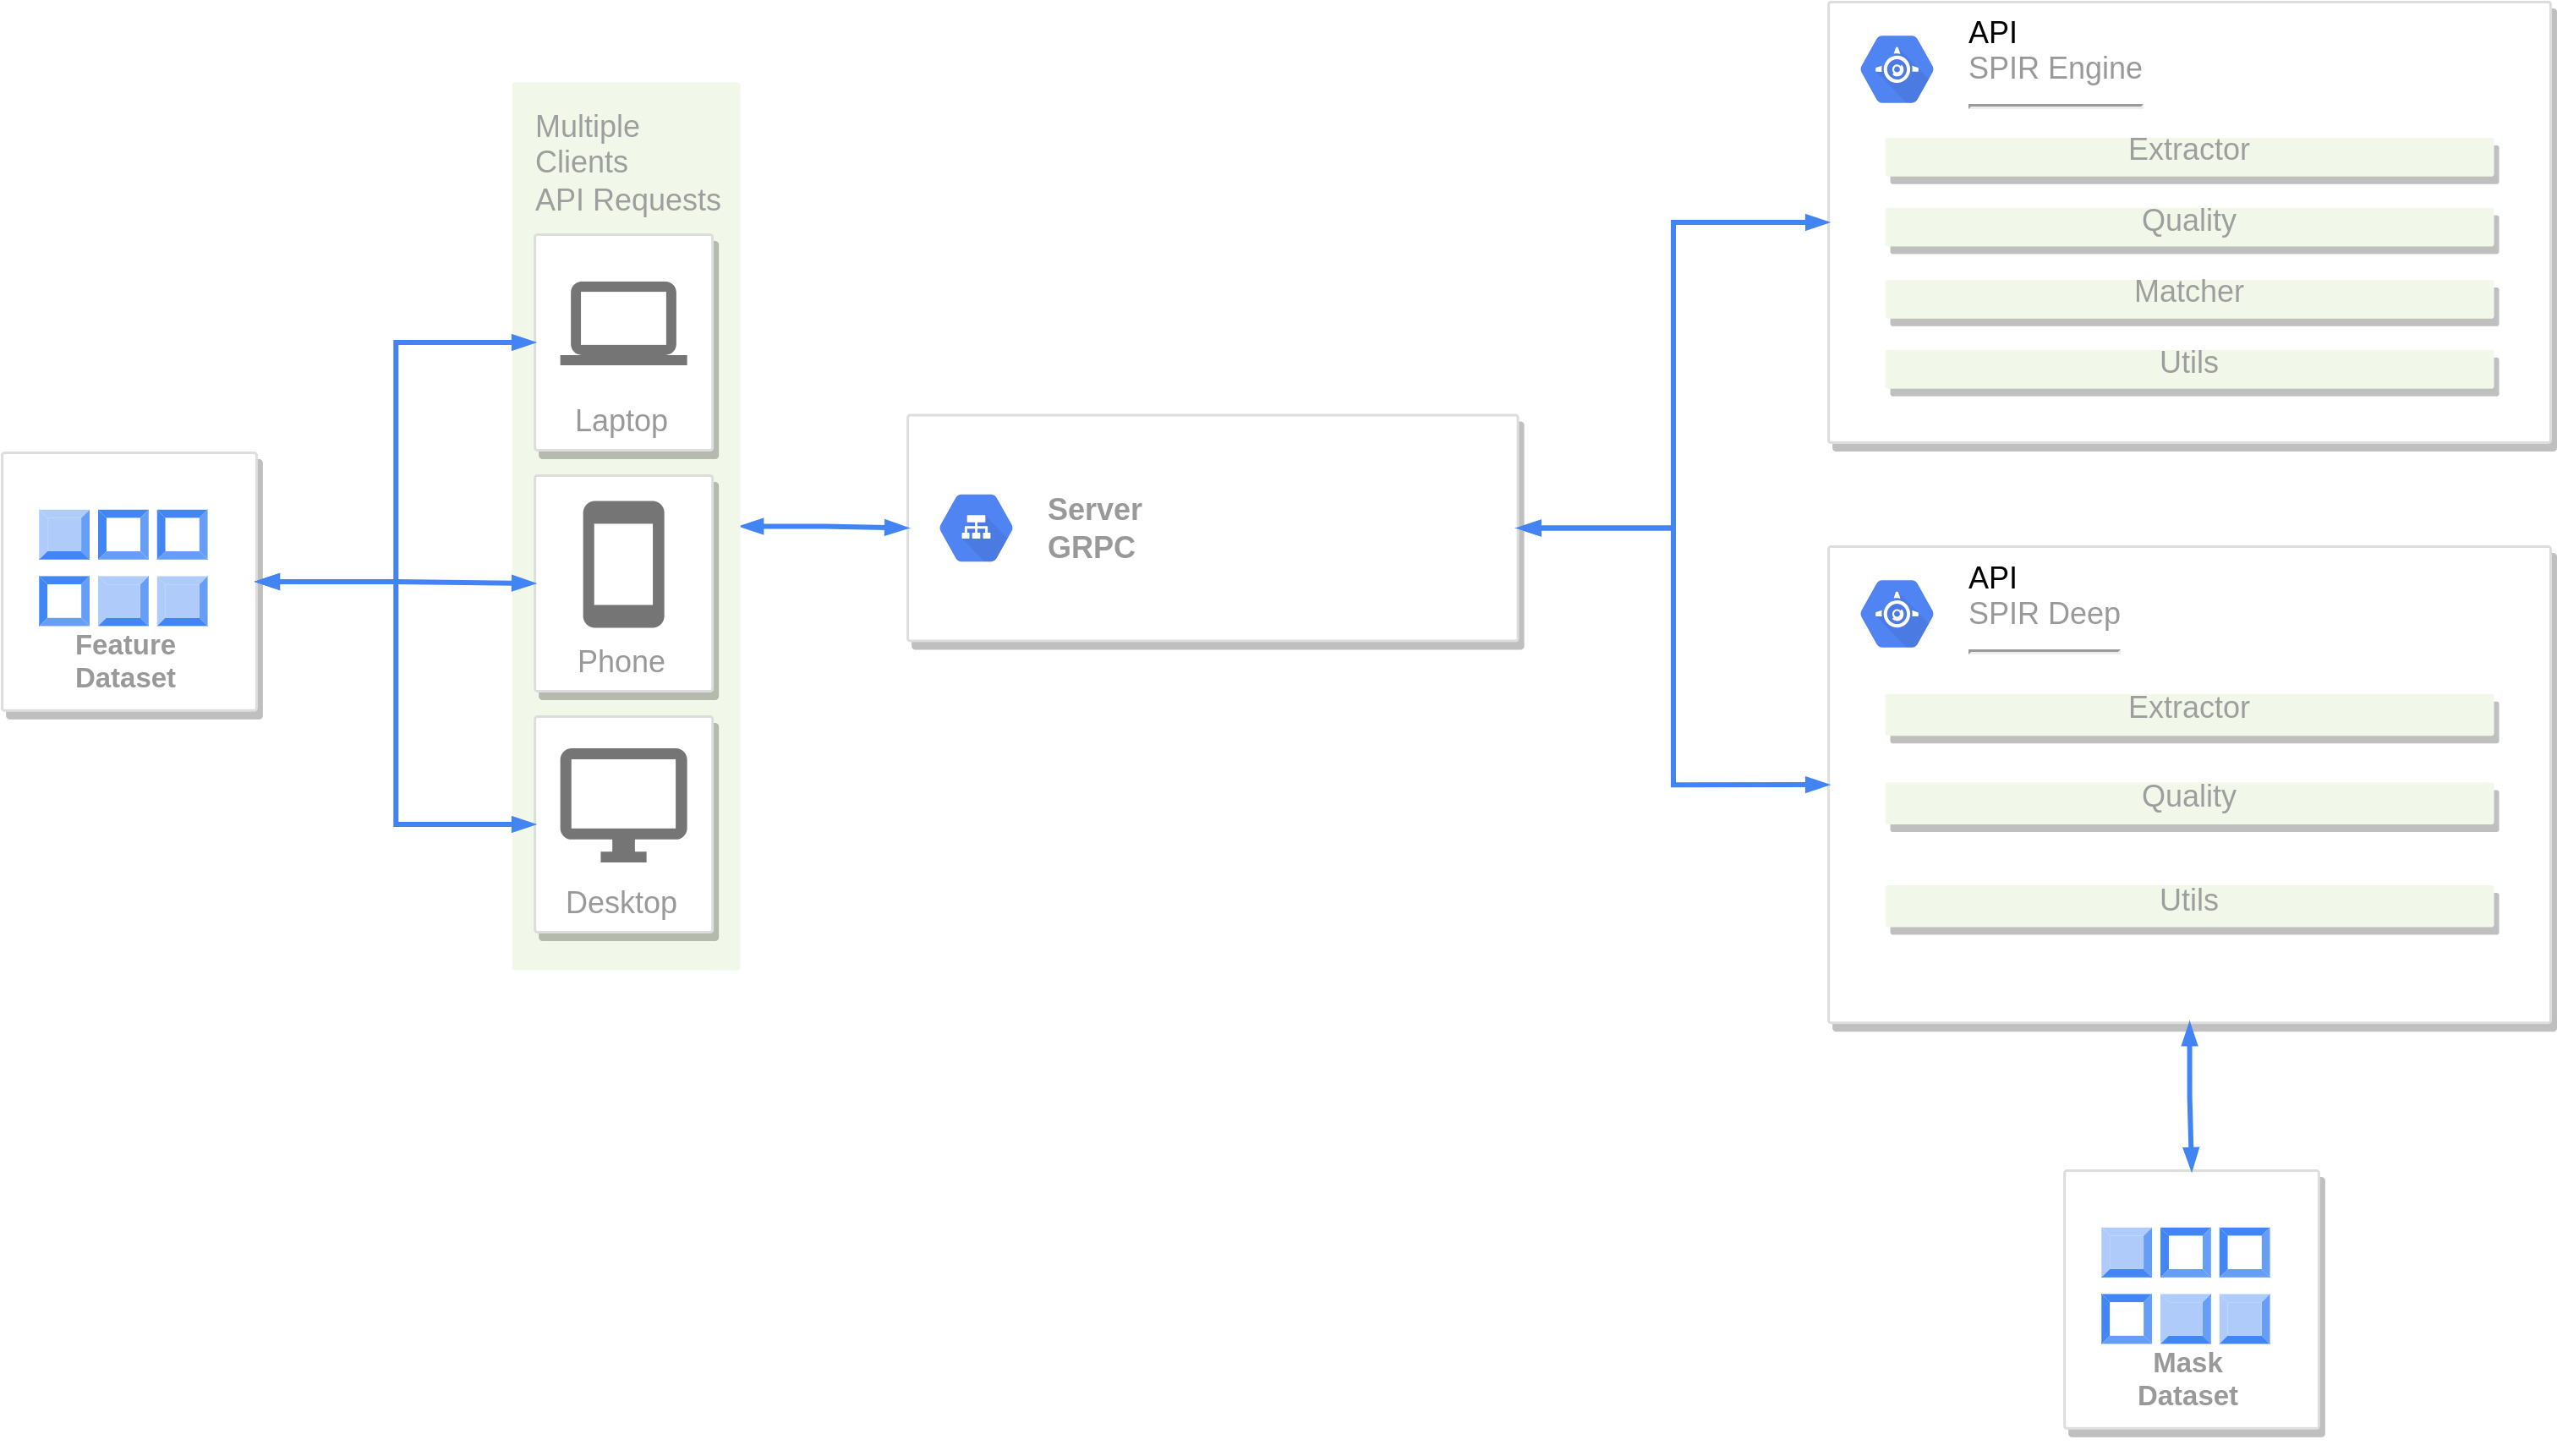
\includegraphics[width=\textwidth]{assets/images/methods/backend/backend_server.drawio.png}   
      \caption{Macro componenti del sistema}
    \end{figure}
    
    \subsection{Architettura}

    L'adozione di un'architettura client/server, con il server responsabile dell'estrazione delle features e del matching, è una scelta strategica che deriva da una serie di fattori chiave. Questa architettura è stata selezionata per garantire una distribuzione efficiente del lavoro, una gestione centralizzata delle funzionalità complesse, un controllo sicuro, una scalabilità ottimale e una migliore interoperabilità.
    La prima ragione fondamentale per cui è stata adottata un'architettura client/server è la distribuzione del carico di lavoro. L'estrazione delle features e il matching possono richiedere risorse computazionali considerevoli, come il tempo di calcolo e la capacità di elaborazione. Distribuire queste operazioni tra client e server permette di bilanciare il carico di lavoro in modo più equo. Il server, con la sua maggiore potenza di calcolo e scalabilità, può dedicarsi all'elaborazione intensiva, mentre il client si concentra sull'interazione con l'utente e sfrutta i risultati ottenuti dal server.
    \\
    In secondo luogo, l'architettura client/server consente una gestione centralizzata delle funzionalità complesse. L'estrazione delle features e il matching richiedono algoritmi sofisticati e un'elaborazione avanzata dei dati. Concentrare queste funzionalità nel server permette di mantenere una base di codice specializzata e centralizzata. Inoltre, gli aggiornamenti o le migliorie all'algoritmo possono essere implementati in modo efficiente sul server, evitando la necessità di apportare modifiche a tutti i client.
    \\
    La scalabilità è un fattore determinante per l'adozione di un'architettura client/server. Affinché il sistema sia in grado di gestire un elevato numero di utenti o un'intensa attività di estrazione delle features e matching, è necessario distribuire il carico di lavoro su più risorse server. Ciò consente di adattarsi alle crescenti esigenze del sistema e di garantire prestazioni affidabili e tempi di risposta rapidi.

    \subsection{Backend}
    gRPC \cite{grpc} è un framework di comunicazione remota sviluppato da Google. È basato su HTTP/2 e utilizza Protocol Buffers (protobuf) come formato di serializzazione dei dati. gRPC offre un modo efficiente e scalabile per la comunicazione tra client e server in un'architettura distribuita. Ecco alcuni dei vantaggi principali di basare un server su gRPC:
    \begin{itemize}
      \item Alta performance: gRPC è progettato per offrire alte prestazioni. Utilizzando HTTP/2 come protocollo di trasporto, supporta la multiplexing delle richieste e delle risposte su una singola connessione. Ciò riduce l'overhead di comunicazione e consente un utilizzo efficiente della larghezza di banda. Inoltre, gRPC offre una serializzazione binaria tramite protobuf, che è molto più leggera e veloce rispetto ad altri formati come JSON o XML.
      \item Supporto per diversi linguaggi di programmazione: gRPC supporta una vasta gamma di linguaggi di programmazione, tra cui C++, Java, Python, Go, e molti altri. Questo permette di sviluppare sistemi distribuiti eterogenei, dove il client e il server possono essere implementati in linguaggi diversi, ma ancora comunicare tra loro in modo trasparente.
      \item Generazione automatica del codice: Utilizzando protobuf come formato di definizione dell'interfaccia di comunicazione, gRPC permette di generare automaticamente il codice necessario per la comunicazione tra client e server. Questo semplifica notevolmente lo sviluppo e riduce la probabilità di errori legati alla gestione della comunicazione.
      \item Supporto per diversi tipi di chiamate: gRPC supporta diversi tipi di chiamate, tra cui chiamate unidirezionali, chiamate client-streaming, chiamate server-streaming e chiamate bidirezionali. Ciò consente di adattare la comunicazione in base alle specifiche esigenze del sistema, consentendo ad esempio l'invio di grandi quantità di dati in modo efficiente o la gestione di flussi di dati continuativi.
      \item Streaming bidirezionale: Uno dei vantaggi distintivi di gRPC è la capacità di supportare lo streaming bidirezionale, in cui client e server possono inviare e ricevere dati in modo asincrono. Questo è particolarmente utile quando si desidera una comunicazione continua e in tempo reale tra client e server, ad esempio durante il trasferimento di flussi di dati in tempo reale o durante l'elaborazione di dati in batch.
    \end{itemize}

    In sintesi, gRPC offre un modo efficiente, scalabile e flessibile per la comunicazione tra client e server. I vantaggi di basare un server su gRPC includono alte prestazioni, supporto per diversi linguaggi di programmazione, generazione automatica del codice, supporto per diversi tipi di chiamate e streaming bidirezionale. Queste caratteristiche rendono gRPC una scelta popolare per lo sviluppo di servizi distribuiti e sistemi scalabili.

    \newpage    
    \subsection{Frontend}
    Flutter \cite{flutter} è stato scelto come framework client per il sistema per diversi motivi chiave.
    Innanzitutto, offre prestazioni native di alta qualità, garantendo che le app sviluppate con Flutter siano veloci, reattive e abbiano un'esperienza utente ottimale. Grazie alla sua architettura, Flutter consente alle app di interagire direttamente con il sistema operativo sottostante, eliminando la necessità di un bridge e garantendo prestazioni ottimali.
    Uno dei fattori principali che ha guidato la scelta del framework è rappresentato dalle prestazioni native di Flutter. Grazie alla sua architettura, Flutter consente alle app di raggiungere prestazioni elevate e reattività, garantendo un'esperienza utente di qualità. Questo è particolarmente importante per un'applicazione che richiede l'estrazione delle features e il matching, in cui la velocità e l'efficienza sono fondamentali.
    \\

    \begin{figure}[H]
      \centering
      \begin{minipage}{0.3\textwidth}
        \centering
        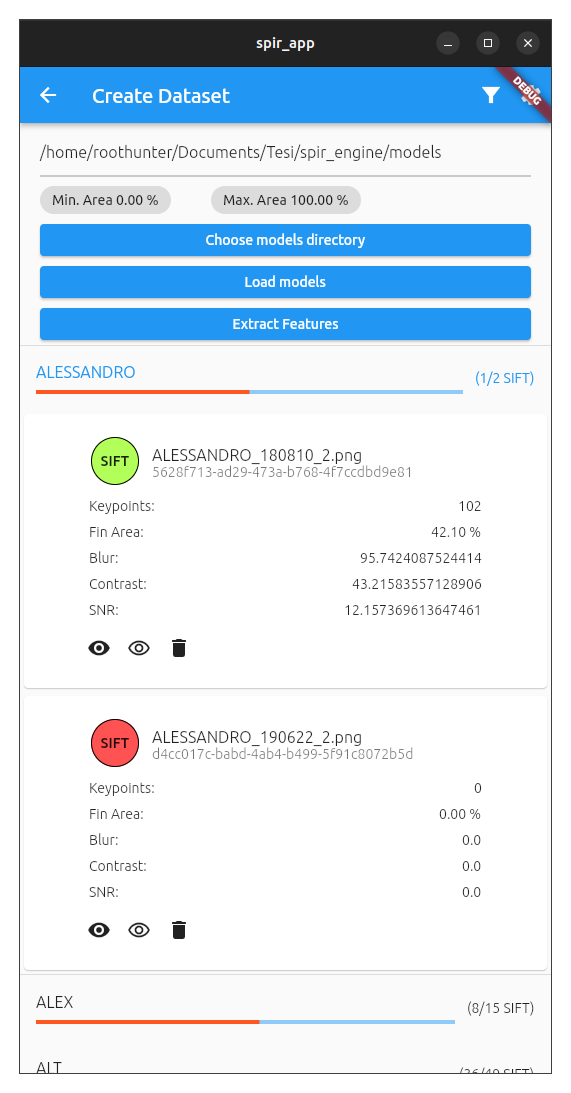
\includegraphics[width=\textwidth]{assets/images/methods/frontend/dataset.png}   
        \caption{Sezione creazione dataset}
      \end{minipage}
      \begin{minipage}{0.3\textwidth}
        \centering
        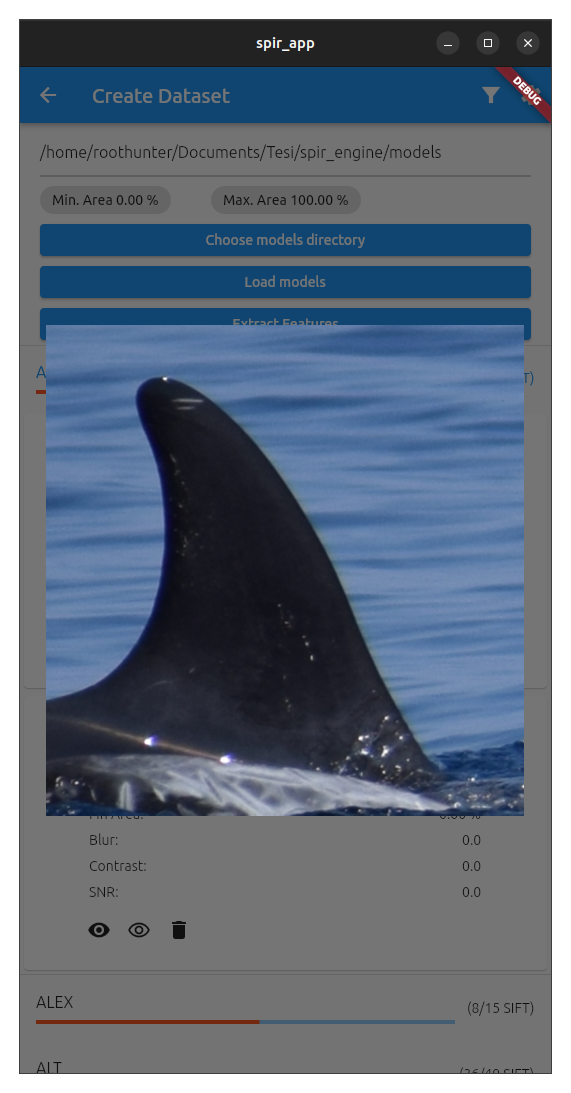
\includegraphics[width=\textwidth]{assets/images/methods/frontend/dataset_image.png}  
        \caption{Anteprima modello}
      \end{minipage}
      \begin{minipage}{0.3\textwidth}
        \centering
        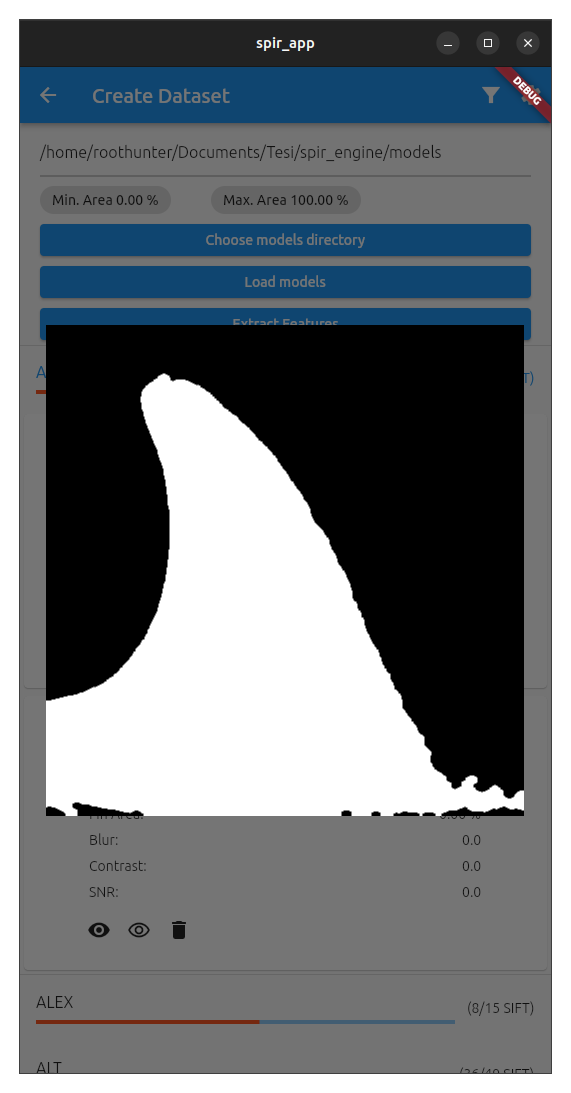
\includegraphics[width=\textwidth]{assets/images/methods/frontend/dataset_mask.png}   
        \caption{Anteprima maschera estratta}
      \end{minipage}
    \end{figure}

    \newpage
      
    L'utilizzo di gRPC in combinazione con Flutter consente una comunicazione efficiente e performante tra il client e il server. In particolare, il supporto per lo streaming bidirezionale offerto da gRPC è vantaggioso per l'estrazione delle features e il matching, consentendo una comunicazione continua tra il client e il server.
    La natura dichiarativa dell'interfaccia utente di Flutter è un altro motivo che ha influenzato la scelta del framework. Con Flutter, l'interfaccia utente viene descritta utilizzando widget, che semplifica la creazione e la personalizzazione di interfacce utente moderne e accattivanti. La funzionalità di Hot Reload di Flutter consente 
     di visualizzare immediatamente le modifiche apportate al codice durante lo sviluppo, consentendo un iterativo e rapido processo di sviluppo.
    \\
    La vasta community di sviluppatori attivi e il supporto continuo offerti da Google sono ulteriori vantaggi che hanno pesato nella scelta di Flutter come framework client. Una community vivace fornisce risorse, documentazione e pacchetti aggiuntivi, facilitando l'apprendimento e l'implementazione di funzionalità aggiuntive nell'applicazione.
    \\
    L'integrazione di TensorFlow in Flutter consente di eseguire inferenze di reti neurali direttamente sui dispositivi dei client, senza dover inviare i dati al server per l'elaborazione. Questa funzionalità potrebbe aprire nuove possibilità per le applicazioni mobili, consentendo loro di sfruttare la potenza delle reti neurali anche in assenza di una connessione Internet o in situazioni in cui la latenza di rete potrebbe essere un problema.
\chapter{Risultati sperimentali}
Lo scopo di questo capitolo è quello di fornire una panoramica completa e accurata dei risultati ottenuti, attraverso la presentazione di dati quantitativi, qualitativi o entrambi, derivanti da esperimenti, osservazioni o analisi condotte. Tale esposizione dei risultati è fondamentale per valutare l'efficacia delle metodologie adottate.
Durante questa analisi e discussione dei risultati, saranno anche evidenziati i limiti dello studio e le possibili fonti di errore o di incertezza che potrebbero aver influenzato i dati ottenuti.
  \section{Confronto tra i diversi approcci}
    \subsection{Estrazione delle maschere}
    \begin{figure}[H]
      \centering
      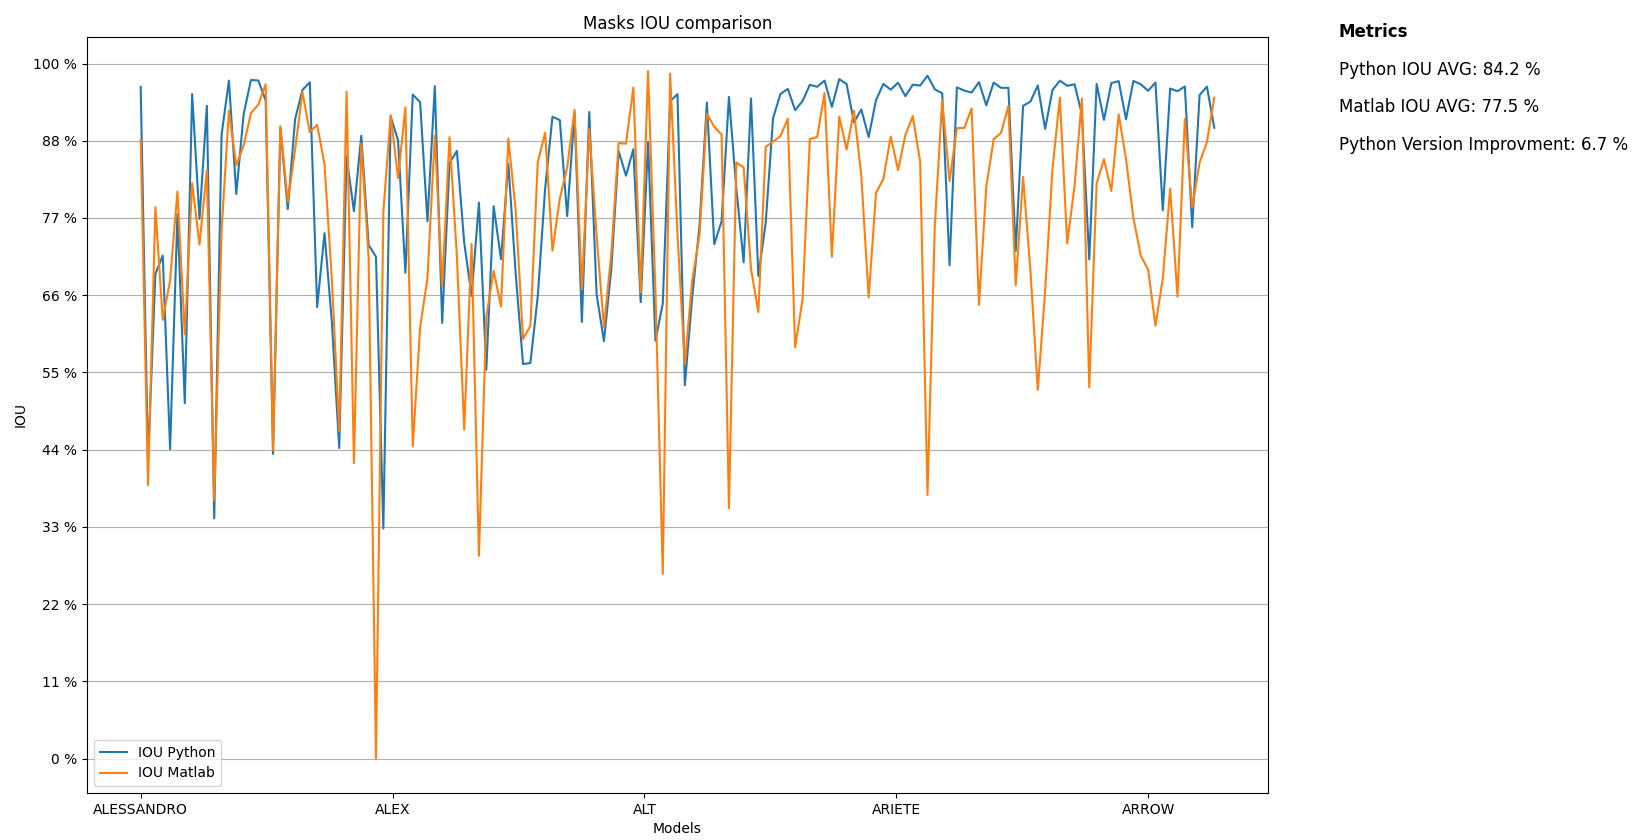
\includegraphics[width=\textwidth]{assets/images/results/result_masks_iou.png}   
      \caption{Confronto IOU}
    \end{figure}
    Per testare e confrontare la nuova implementazione dell'estrazione delle maschere di pinne di delfino fatta in Python rispetto alla versione del sistema SPIR precedente basata su MATLAB, è stata utilizzata come metrica l'IOU (Intersection over Union). L'IOU è una misura di similarità tra due regioni, comunemente utilizzata per valutare la qualità delle maschere generate dai modelli di segmentazione.

    L'IOU viene calcolato dividendo l'area dell'intersezione tra due regioni per l'area dell'unione tra le stesse regioni. In questo contesto, le regioni corrispondono alle maschere poligonali che rappresentano le pinne di delfino. Un valore di IOU pari a 1 indica una perfetta sovrapposizione tra le due maschere, mentre un valore di 0 indica che le maschere non hanno regioni in comune.

    Per confrontare le due versioni di implementazione, è stato utilizzato un dataset di maschere poligonali precedentemente creato per addestrare il modello di deep learning. Questo dataset rappresenta diverse immagini di pinne di delfino, con le relative maschere di riferimento.

    Per ogni immagine nel dataset, sia l'implementazione in Python che la versione in MATLAB sono state utilizzate per estrarre le maschere delle pinne. Successivamente, è stato calcolato l'IOU tra le maschere estratte e le maschere di riferimento presenti nel dataset.

    Infine, è stato possibile confrontare le due versioni del sistema SPIR calcolando la media degli incrementi dell'IOU per l'implementazione Python rispetto all'IOU ottenuta per la versione originale di SPIR in MATLAB.
    È emerso che l'implementazione in Python ha mostrato un incremento medio dell'IOU di circa il 6\% rispetto alla versione di SPIR in MATLAB (vedi Figura 3.1).
    Questo suggerisce che la nuova implementazione in Python ha prodotto maschere di pinne di delfino più accurate e simili alle maschere di riferimento presenti nel dataset.

    \begin{figure}[H]
      \centering
      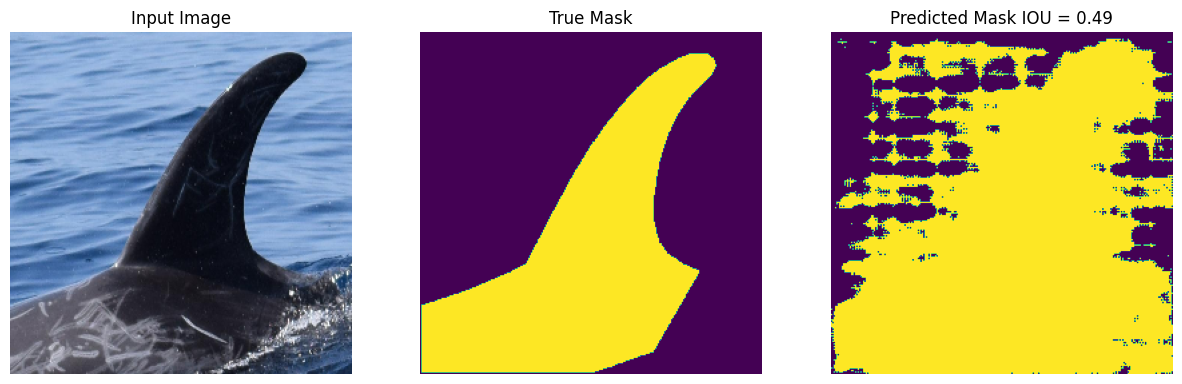
\includegraphics[width=\textwidth]{assets/images/results/result_mask_deep.png}   
      \caption{Confrontro maschera predetta dall'IA}
    \end{figure}
    L'utilizzo di una rete neurale profonda (deep neural network) per l'estrazione delle maschere potrebbe non aver raggiunto i risultati aspettati rispetto ai metodi precedenti, ovvero l'implementazione in Python e quella in MATLAB. Ciò potrebbe essere attribuito principalmente alla dimensione limitata del dataset utilizzato per addestrare la rete neurale.
    \\
    Il fatto che il dataset di addestramento contenga solo 150 immagini con le relative maschere poligonali potrebbe non essere sufficiente per catturare la complessità e la varietà delle pinne di delfino presenti nelle foto. Le reti neurali profonde, soprattutto quando addestrate con un numero limitato di dati, possono essere soggette a problemi di generalizzazione e potrebbero non essere in grado di apprendere efficacemente le caratteristiche discriminanti delle pinne.
    \\
    Nel tentativo di affrontare questa sfida, sono state applicate tecniche di data augmentation, che consentono di generare ulteriori dati di addestramento modificando in modo intelligente le immagini esistenti. Tuttavia, nonostante l'uso di queste tecniche, l'IOU ottenuto con la rete neurale deep non supera il valore di 0.55.
    In conclusione, l'incapacità della rete neurale deep di raggiungere i risultati dei metodi precedenti (Python e MATLAB) potrebbe essere attribuita alla dimensione limitata del dataset di addestramento e alla conseguente difficoltà di apprendimento delle caratteristiche discriminanti delle pinne di delfino. L'acquisizione di un dataset più ampio e l'implementazione di strategie di addestramento più avanzate potrebbero essere necessarie per superare questa sfida e migliorare le prestazioni della rete neurale deep nell'estrazione delle maschere.
    \newpage

    \subsection{Matching features}
    \begin{figure}[H]
      \centering
      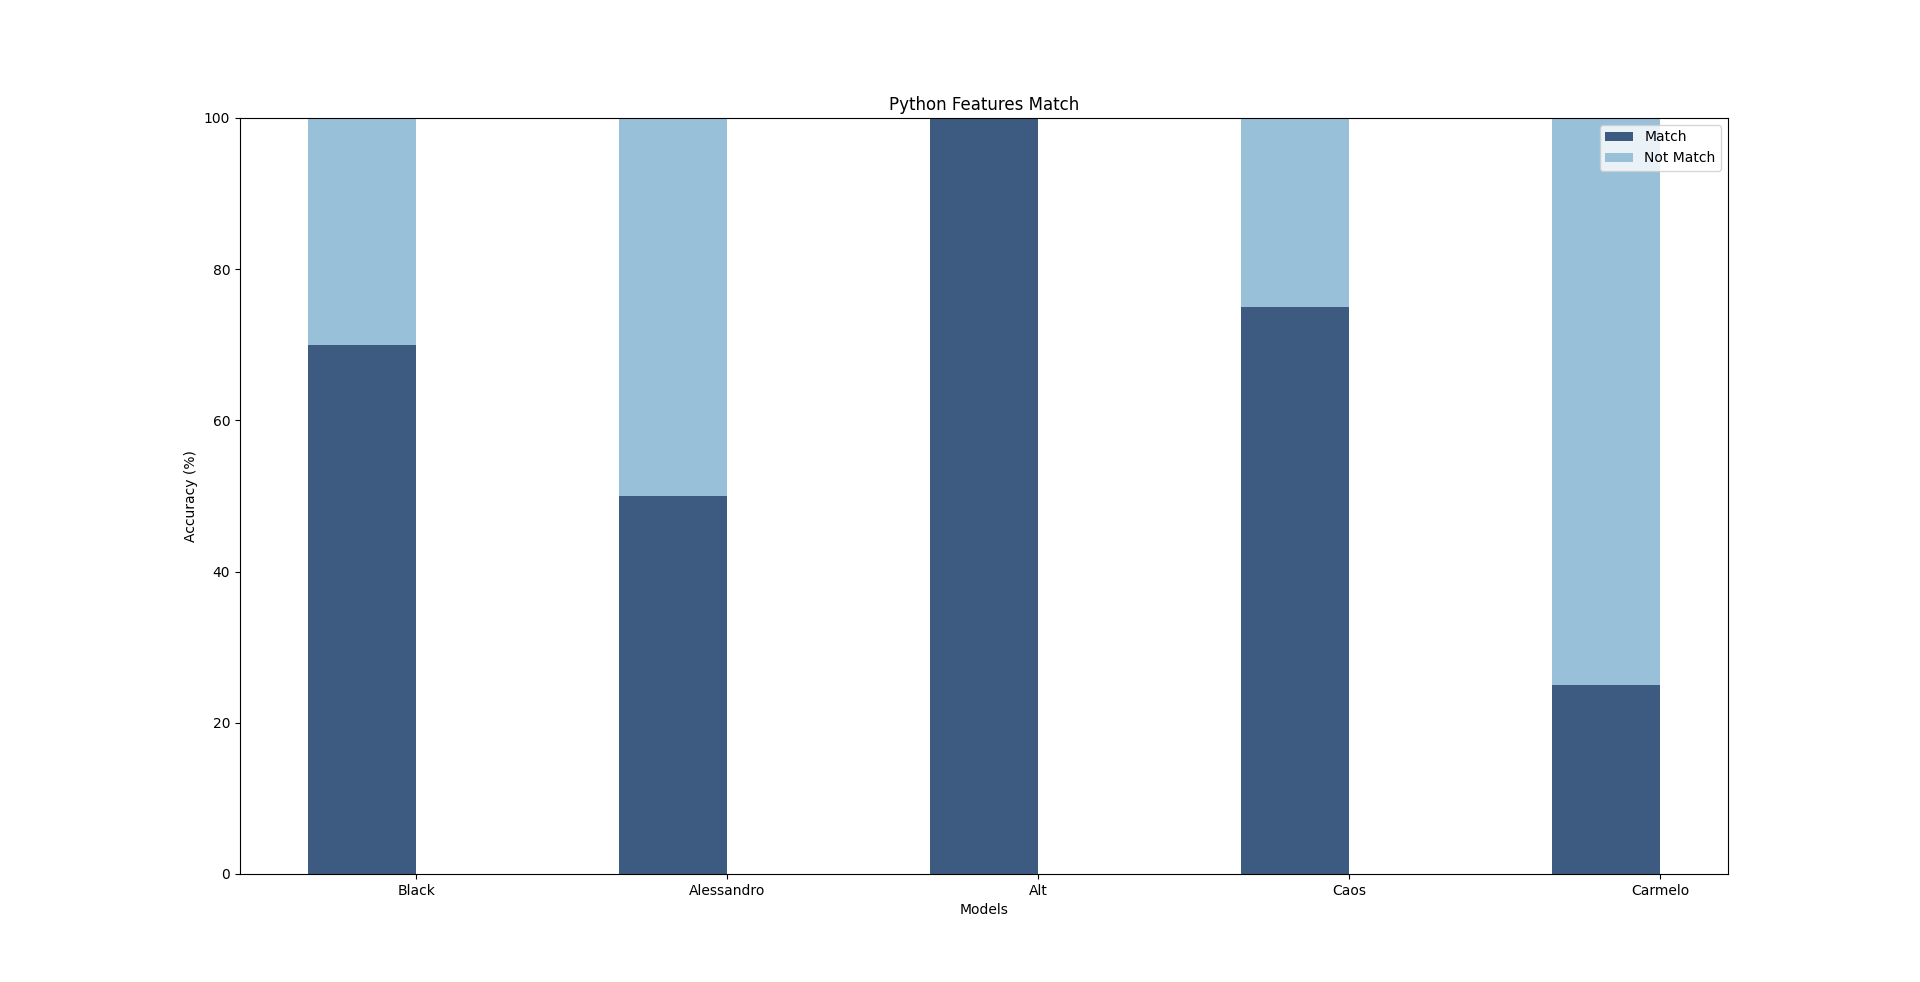
\includegraphics[width=\textwidth]{assets/images/results/result_match.png}   
      \caption{Python SPIR matches}
    \end{figure}

    La versione Python del sistema SPIR ha mostrato risultati promettenti in termini di match delle feature. Grazie all'implementazione ottimizzata e alle migliorate tecniche di estrazione delle maschere, il sistema è stato in grado di ottenere un alto tasso di successo nel match delle feature tra le immagini di delfini.
    I risultati positivi ottenuti con la versione Python di SPIR hanno aperto nuove prospettive e opportunità per l'applicazione del sistema. La sua efficacia nel riconoscimento dei delfini attraverso le feature delle pinne può essere sfruttata in diversi ambiti, come la ricerca e il monitoraggio delle popolazioni di delfini, la conservazione della fauna marina e la gestione degli habitat.
    Inoltre, i risultati dei match ottenuti con la versione Python di SPIR consentono anche di considerare l'integrazione del sistema in altre piattaforme e ambienti. La flessibilità e la portabilità offerte dalla versione Python consentono di adattare il sistema per l'utilizzo su dispositivi mobili o in ambienti distribuiti, aprendo nuove prospettive per l'applicazione pratica del sistema nel campo della ricerca e della conservazione dei delfini.
    È importante notare che, nonostante i risultati promettenti ottenuti con la versione Python di SPIR, ci sono casi in cui non riesce a superare le prestazioni della versione Matlab. Questo apre interessanti scenari per futuri miglioramenti e ottimizzazioni della fase di match delle feature.

    Sebbene la versione Python di SPIR abbia dimostrato buone prestazioni nella maggior parte dei casi, ci sono situazioni (CARMELO) in cui la versione Matlab ha mostrato un margine di miglioramento rispetto alla precisione del match delle feature. Questo può essere dovuto a varie ragioni, come differenze nell'implementazione degli algoritmi o nell'ottimizzazione delle operazioni.
    
    \newpage
    \subsection{Prestazioni}
    Specifiche ambiente di test:

    \begin{itemize}
      \item Processore: AMD 4800H
      \item CPU Cores: 8
      \item Threads: 16
      \item RAM: 48 GB
      \item GPU: NVIDIA GTX 1650 Ti
      \item VRAM: 4 GB
      \item OS: Ubuntu 23.04
      \item Linux Kernel: 6.2.16
      \item Python: 3.10.11
      \item MATLAB: R2023a
    \end{itemize}

    La nuova implementazione del modulo di estrazione delle maschere scritta in Python ha dimostrato un notevole miglioramento sia in termini di tempo di esecuzione che di qualità delle maschere rispetto alla precedente implementazione basata su MATLAB. Questi risultati sono stati ottenuti grazie all'utilizzo di tecniche più efficienti e all'ottimizzazione delle operazioni di elaborazione delle immagini.

    \begin{figure}[H]
      \centering
      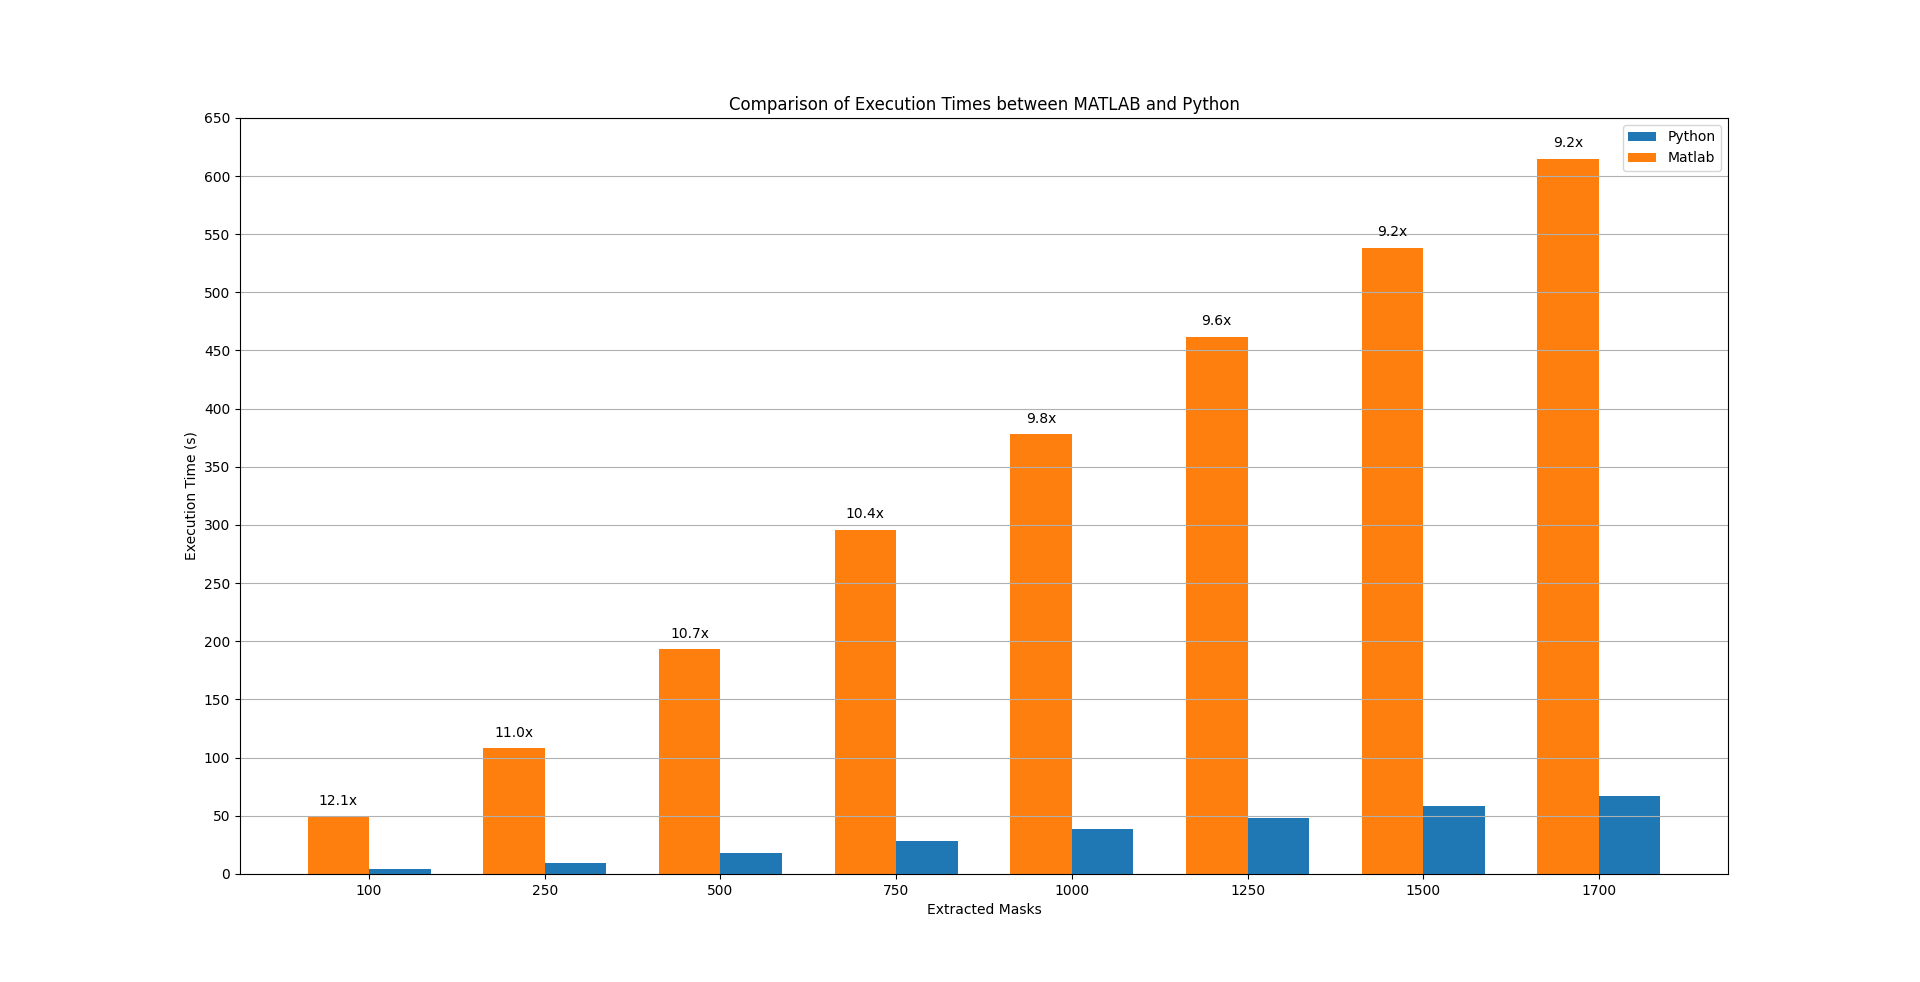
\includegraphics[width=\textwidth]{assets/images/results/result_execution_time.png}   
      \caption{Tempi di esecuzione estrazione maschere}
    \end{figure}
    
    Iniziamo analizzando il tempo di esecuzione. La nuova implementazione in Python è riuscita ad accelerare significativamente il processo di estrazione delle maschere rispetto a quella basata su MATLAB. Con un tempo di esecuzione fino a 12 volte minore, il sistema è diventato notevolmente più efficiente, consentendo di analizzare un maggior numero di immagini nel medesimo intervallo di tempo. Questo rappresenta un vantaggio significativo in termini di produttività e possibilità di scalabilità del sistema.
    
  

    L'implementazione in Python ha portato vantaggi significativi anche in termini di dimensione del dataset contenente le feature rispetto alla versione precedente basata su MATLAB. Infatti, grazie a diverse ottimizzazioni e modifiche apportate al modo di gestire i dati durante la fase di salvataggio, è stato possibile ottenere un notevole miglioramento delle dimensioni del dataset.
    Uno dei principali fattori che hanno contribuito a questa riduzione della dimensione del dataset è stata l'adozione di una libreria di serializzazione/deserializzazione chiamata Protocol Buffers (protobuf).
    \\
    Utilizzando protobuf, è stato possibile ristrutturare il modo in cui le feature venivano salvate nel dataset, eliminando informazioni ridondanti o non necessarie e utilizzando un formato più compatto. Questa ottimizzazione ha portato a un notevole risparmio di spazio e ha permesso di ridurre considerevolmente la dimensione complessiva del dataset.
    Questa significativa riduzione delle dimensioni del dataset non solo ha comportato un risparmio di spazio di archiviazione, ma ha anche portato a un notevole miglioramento delle prestazioni del sistema. La riduzione della quantità di dati da elaborare ha permesso di accelerare i tempi di esecuzione delle operazioni di caricamento e salvataggio delle feature, contribuendo a una maggiore efficienza complessiva del sistema.
    
    \begin{figure}[H]
      \centering
      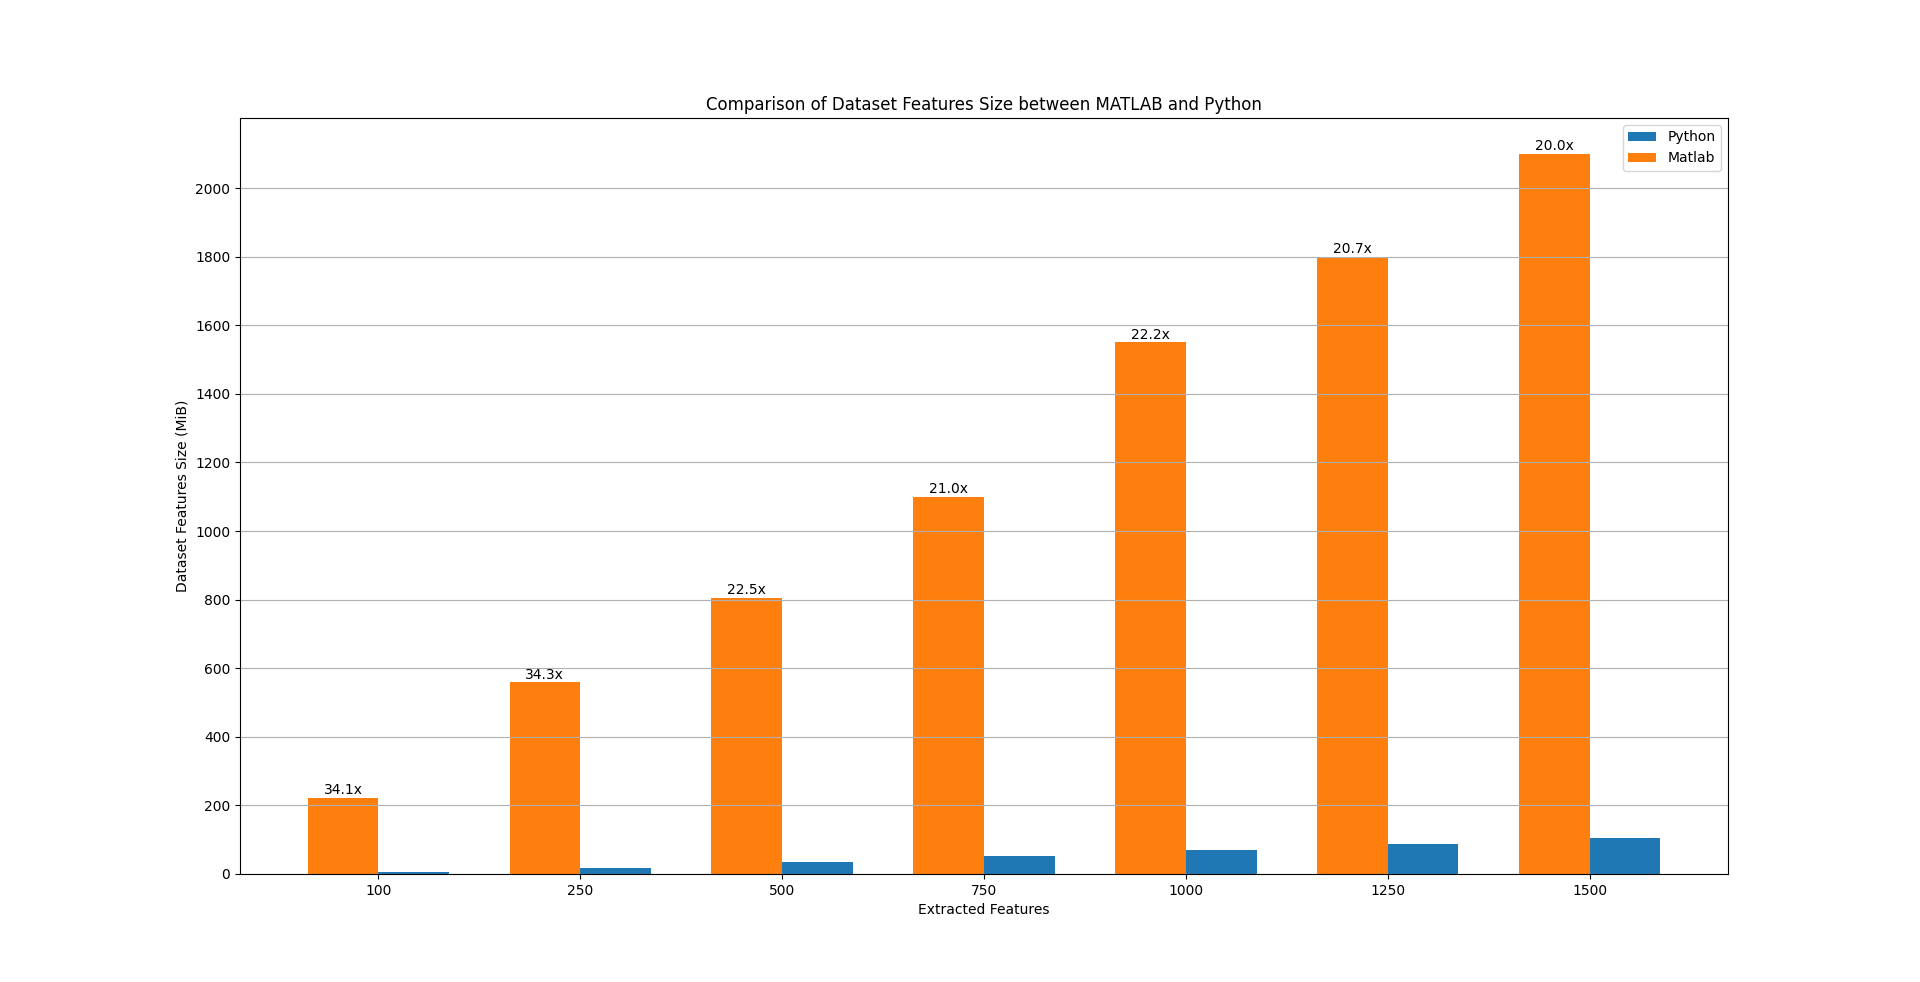
\includegraphics[width=\textwidth]{assets/images/results/result_dataset_size.png}   
      \caption{Dimensione del dataset di feature}
    \end{figure}

    L'impressionante miglioramento della dimensione del dataset e dei tempi di esecuzione ottenuto grazie all'implementazione in Python ha aperto interessanti opportunità per l'architettura client/server e l'adozione di dispositivi mobili.

    L'adozione di dispositivi mobili viene favorita dalla riduzione delle dimensioni del dataset e dai tempi di elaborazione più rapidi. La riduzione della quantità di dati da trasferire e processare consente ai dispositivi mobili di utilizzare meno risorse, come la larghezza di banda e la potenza di calcolo, preservando la durata della batteria e migliorando le prestazioni complessive dell'applicazione. Inoltre, i dispositivi mobili possono beneficiare dell'elaborazione in tempo reale delle feature estratte, consentendo esperienze interattive e immediate per gli utenti.
    Grazie alla riduzione delle dimensioni del dataset, il trasferimento dei dati tra client e server diventa più efficiente. I dati compressi possono essere trasmessi più rapidamente attraverso la rete, riducendo la latenza e migliorando l'esperienza utente. Ciò rende l'architettura client/server ancora più adatta per applicazioni che richiedono l'elaborazione di grandi quantità di dati, come ad esempio l'identificazione automatica delle foto di cui si sta discutendo.
\chapter{Conclusioni}
  \section{Riepilogo degli obiettivi raggiunti}
    Durante lo studio e il porting del sistema di foto identificazione automatica SPIR da MATLAB a Python, sono stati raggiunti diversi obiettivi. L'obiettivo principale era realizzare il porting della versione originale del sistema SPIR utilizzando il linguaggio di programmazione Python. Ciò è stato ottenuto con successo, consentendo di beneficiare delle numerose librerie e dell'ampia comunità di sviluppatori associate a Python.
    Inoltre, è stato sviluppato un'interfaccia grafica user-friendly per il sistema SPIR. L'adozione di un'interfaccia grafica offre diversi vantaggi, tra cui una maggiore facilità d'uso e accessibilità per gli utenti. Ciò apre nuovi scenari di utilizzo per il sistema SPIR, consentendo a una gamma più ampia di utenti, incluso il personale non tecnico, di sfruttarne le funzionalità.
    In conclusione, lo studio e il porting di SPIR da MATLAB a Python hanno raggiunto gli obiettivi prefissati, consentendo di beneficiare delle caratteristiche e delle risorse offerte da Python. L'adozione di un'interfaccia grafica user-friendly amplia le possibilità di utilizzo del sistema, rendendolo accessibile a un pubblico più vasto e aprendo nuove prospettive per il suo impiego in contesti reali.

  \section{Possibili sviluppi futuri}
  I possibili sviluppi futuri per il sistema SPIR includono diverse direzioni che potrebbero portare a ulteriori miglioramenti e vantaggi. Alcune di queste direzioni potrebbero riguardare l'ulteriore sviluppo e miglioramento della rete neurale profonda utilizzata per l'estrazione delle maschere.
  Uno dei potenziali miglioramenti potrebbe riguardare l'ottimizzazione e l'adattamento della rete neurale profonda per raggiungere una maggiore precisione nell'estrazione delle maschere. Ciò potrebbe comportare l'aggiunta di ulteriori strati o l'utilizzo di architetture più complesse, nonché l'adeguamento dei parametri di allenamento per ottenere risultati ancora migliori. Questo consentirebbe di ottenere maschere più precise e di alta qualità, migliorando ulteriormente le prestazioni globali del sistema SPIR.
  Inoltre, un'altra prospettiva interessante potrebbe essere l'utilizzo dei dispositivi mobili per l'inferenza sulle maschere. Con l'avanzamento dell'hardware specializzato per l'intelligenza artificiale nei dispositivi mobili, come le unità di elaborazione neurali (NPU) integrate nei chip dei telefoni, sarebbe possibile eseguire l'inferenza delle maschere direttamente sui dispositivi stessi. Ciò comporterebbe notevoli vantaggi in termini di tempi di elaborazione e riduzione della dipendenza da risorse esterne, consentendo un'esperienza più rapida e reattiva per gli utenti.

  \bibliographystyle{plain}
  \bibliography{bibliography}
\end{document}